\documentclass[11pt,a4paper,oneside]{memoir}
\usepackage[utf8]{inputenc}
\usepackage{gensymb}
\usepackage{helvet}
\usepackage{multirow}
\usepackage{amsmath}
\usepackage{algorithm}
\usepackage{algpseudocode}
\usepackage{amssymb}
\usepackage{verbatim}
\usepackage[
breaklinks=true,colorlinks=true,
%linkcolor=blue,urlcolor=blue,citecolor=blue,% PDF VIEW
linkcolor=black,urlcolor=black,citecolor=black,% PRINT
bookmarks=true,bookmarksopenlevel=2]{hyperref}
\usepackage[
    backend = biber,
    style = numeric,
]{biblatex}
\addbibresource{Bibliography.bib}
\usepackage{standalone}

\usepackage{geometry}
\geometry{
    left=2cm, % Adjust left margin
    right=2cm, % Adjust right margin
    top=2.5cm, % Adjust top margin
    bottom=2.5cm, % Adjust bottom margin
}

\OnehalfSpacing
%\linespread{1.3}

%%% CHAPTER'S STYLE
%\chapterstyle{bianchi}
\chapterstyle{brotherton}
%\chapterstyle{madsen}
%\chapterstyle{ell}

%%% STYLE OF PAGES NUMBERING
\pagestyle{plain}
\makepagestyle{plain}
\makeevenfoot{plain}{\thepage}{}{}
\makeoddfoot{plain}{}{}{\thepage}
\makeevenhead{plain}{}{}{}
\makeoddhead{plain}{}{}{}


\maxsecnumdepth{subsection} % chapters, sections, and subsections are numbered
\maxtocdepth{subsection} % chapters, sections, and subsections are in the Table of Contents

\usepackage{tikz}
\addbibresource{Bibliography.bib}
\usepackage{amsthm}

\theoremstyle{plain}
\newtheorem{theorem}{Theorem}[chapter] % reset theorem numbering for each chapter

\theoremstyle{plain}
\newtheorem{lemma}[theorem]{Lemma}

\theoremstyle{plain}
\newtheorem{corollary}[theorem]{Corollary}

\theoremstyle{definition}
\newtheorem{definition}[theorem]{Definition} % definition numbers are dependent on theorem numbers

\newtheorem{example}[theorem]{Example} % same for example numbers

%% tikz packages
\usepackage{pgfmath, pgffor}
\usepackage{caption}
\DeclareCaptionFormat{myformat}{\fontsize{10pt}{10pt}\selectfont\setlength{\baselineskip}{16pt}#1#2#3} % Adjust the font size and line spacing here
\captionsetup{format=myformat, skip=2pt} % Adjust the skip value here
\usepackage{subcaption}
\usepackage{tikz}
\usetikzlibrary{arrows,backgrounds,positioning,petri, calc}

% allow for hyperlinks
\usepackage{hyperref}

% dark mode
\usepackage{xcolor}
%\pagecolor[rgb]{0.101,0.101,0.18}
%\color[rgb]{0.8,0.8,0.8}

\usepackage{fancyhdr}

% Set up fancy headers and footers
\pagestyle{fancy}
\fancyhf{} % Clear default header and footer
\fancyfoot[C]{\thepage} % Center the page number
\renewcommand{\headrulewidth}{0pt} % Remove the header rule

% Redefine the plain page style for chapter pages
\fancypagestyle{plain}{%
  \fancyhf{} % Clear header and footer
  \fancyfoot[C]{\thepage} % Center the page number
  \renewcommand{\headrulewidth}{0pt} % Remove the header rule
}

% for grey background when listing code
\usepackage{listings,color}
\definecolor{verbgray}{gray}{0.9}
\lstnewenvironment{code}{%
  \lstset{
    backgroundcolor=\color{verbgray},
    frame=single,
    framerule=0pt,
    basicstyle=\small\ttfamily, % Adjust the font size here
    columns=fullflexible
  }
}{}




\begin{document}

% tikz styles
\tikzstyle{vertex} = [circle, draw=black, fill = black, thin, inner sep=0pt,minimum size=2mm]

\tikzstyle{origin} = [circle, draw=black, fill = black, thin, inner sep=0pt,minimum size=1mm]

%   TITLEPAGE

\thispagestyle{empty}

{%%%

\centering
\Large

~\vspace{\fill}

%** Figure out a better title
{\huge 
Minimally Rigid Graphs and their Circle Packings: A Rigid Investigation
}

\vspace{2.5cm}

{\LARGE
Ritwik Rajaram Anand
}

\vspace{3.5cm}


School of Mathematics and Statistics\\
University of St Andrews

\vspace{3.5cm}

\vspace{\fill}

\date{April 2024}

%%%
}%%%

\cleardoublepage

%----------------------------------------------------------------------
% figure out how to center abstract
\section*{Abstract}    
TBD

\section*{Declaration}
\textit{I certify that this project report has been written by me, is a record of work
carried out by me, and is essentially different from work undertaken for any
other purpose or assessment}.

\clearpage

%----------------------------------------------------------------------

\tableofcontents*

\clearpage


%----------------------------------------------------------------------

\chapter{Introduction}

\begin{flushleft}
The circle is arguably the most fundamentally studied mathematical object in history. In fact, the construction of the unit circle dates all the way back to the second century BC \cite{unit_circle}. With this elementary object, we are able obtain two trigonometric functions, enabling us to study a myriad of physical processes such as the motion of waves and the oscillatory properties of pendulums. In this project however, we will be looking less at the properties of the circle, and more on various geometries involved when we attempt to group, or \textit{pack} as many as we can together. 
\end{flushleft}

\begin{flushleft}
As some motivation for what is to come, let us take a stroll down the fruits and vegetables section at the supermarket. While looking around, we notice that spherical fruit, such as oranges, are stacked high in a in a pyramidal-like shape that tapers off at the top. A display like this is known as a \textit{face-centered cubic packing}.
\end{flushleft}

\begin{figure}[htbp]
    \centering
    \begin{tabular}{c c}
      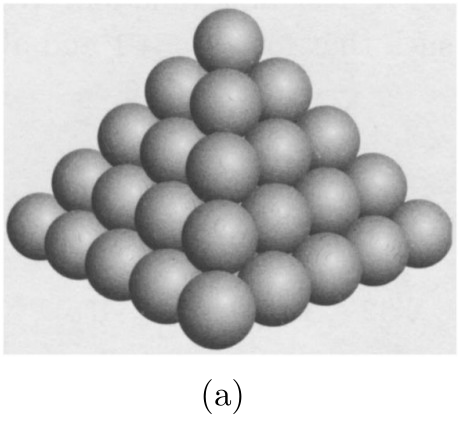
\includegraphics[width = 0.35\textwidth]{Chapter 1/2. Cubic packing.png}   & 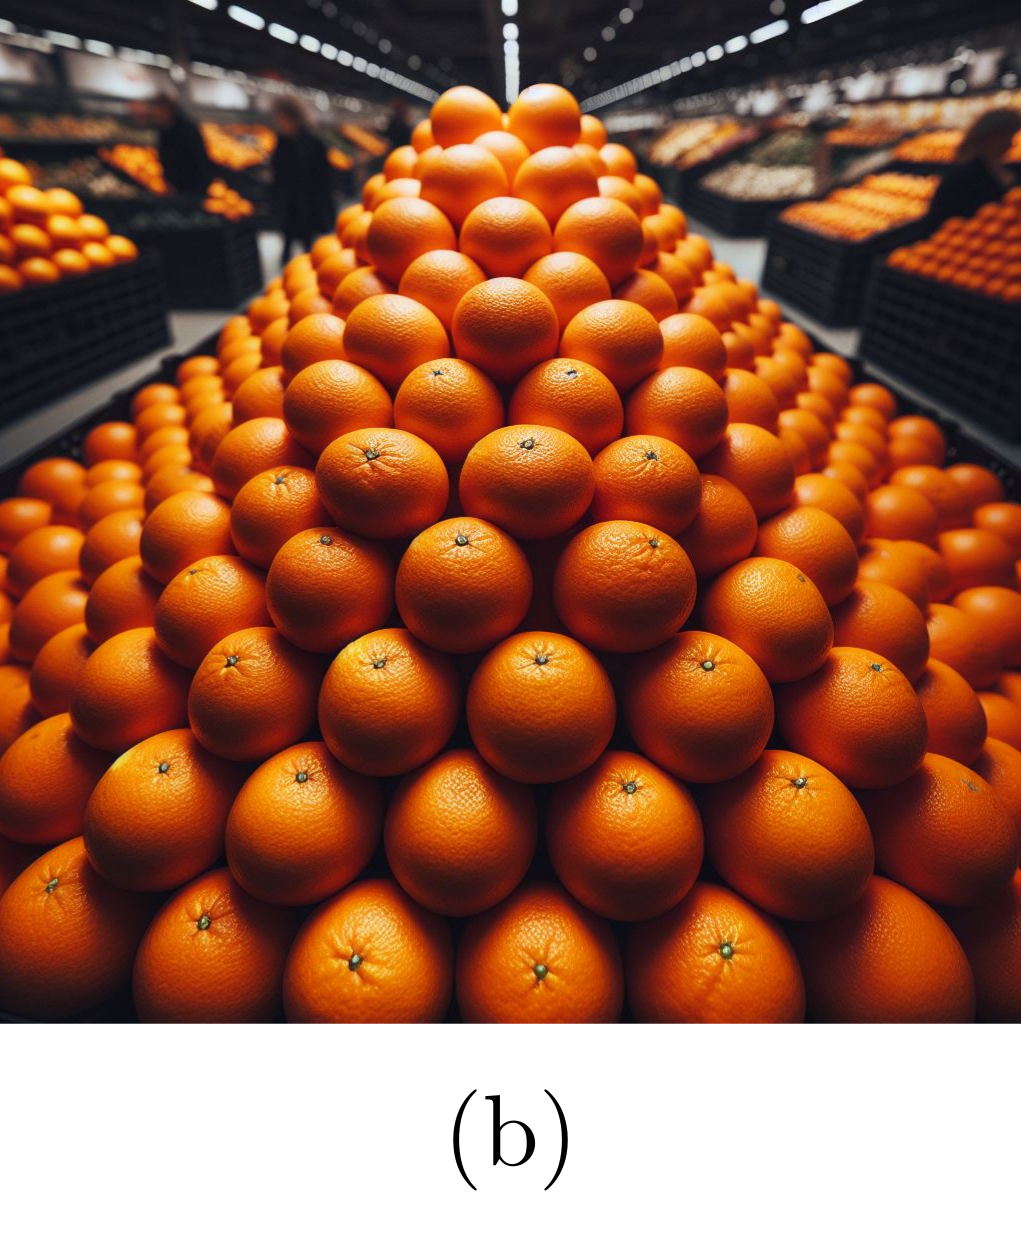
\includegraphics[width = 0.275\textwidth]{Chapter 1/oranges.png}
    \end{tabular}
    \caption{(a) A face-centered cubic packing, taken from \cite{kepler}. (b) An image of oranges stacked in a face-centered cubic packing, generated by DALL·E 3.}
\end{figure}
\vspace{-4 mm}
\begin{flushleft}
This interesting observation was studied by Johannes Kepler, who attempted to find the optimal way to stack cannonballs. In 1611, Kepler conjectured that a face-centered cubic packing is the most efficient method to stack spheres in 3-dimensional space. This was proved by Thomas Hales, at first using computational methods in 1998, and a formal proof was accepted in 2017 \cite{Kepler_proof}.
\end{flushleft}

\begin{flushleft}
Going back to the 2-dimensional circle, our interest lies in a \textit{circle packing}, which involves arranging several circles in the plane such that they may only touch tangentially, and there is no overlap between any of the circles. By imposing different constraints, we can generate circle packings where the arrangement formed has circles packed together with a variety of radii, producing an aesthetically pleasing image to regard. They can also be used to study the world around us under a different lens. An example of this involves modelling the arrangement of particles in a crystalline structure as a tight packing of circles \cite{crystalline}.
\end{flushleft}

\begin{flushleft}
By marking the center of each circle in a circle packing, and joining centers with a line if the circles they inhabit are tangential to each other, we are able to construct the packing's \textit{contact graph}, effectively converting our geometric problem into a graph theoretic one. This allows us to use tools from Graph Theory, increasing the size of our repertoire.    
\end{flushleft}

\begin{figure}[htbp]
    \centering
    \begin{tabular}{c c}
        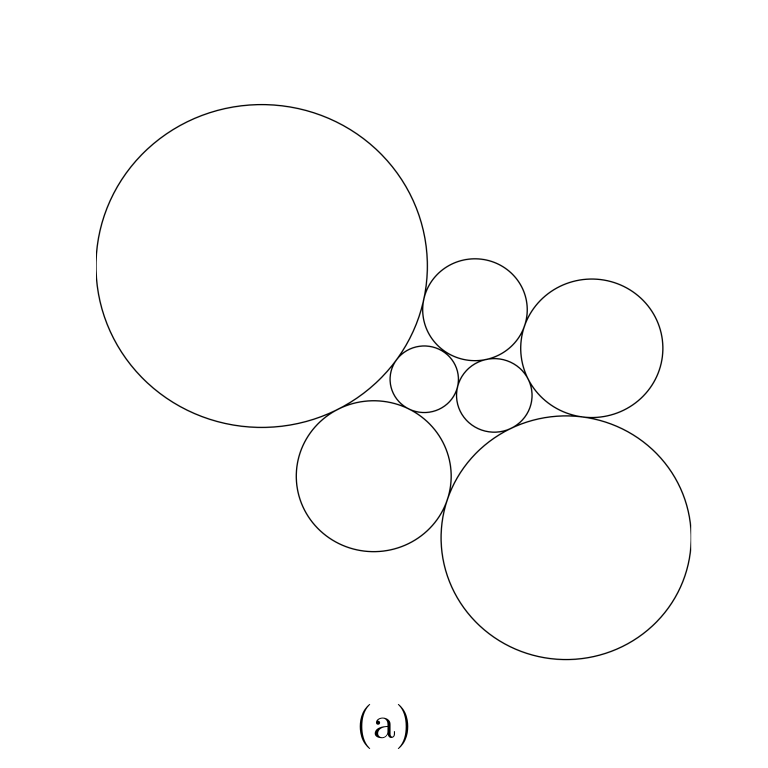
\includegraphics[width = 0.4\textwidth]{Chapter 1/packing.png} & 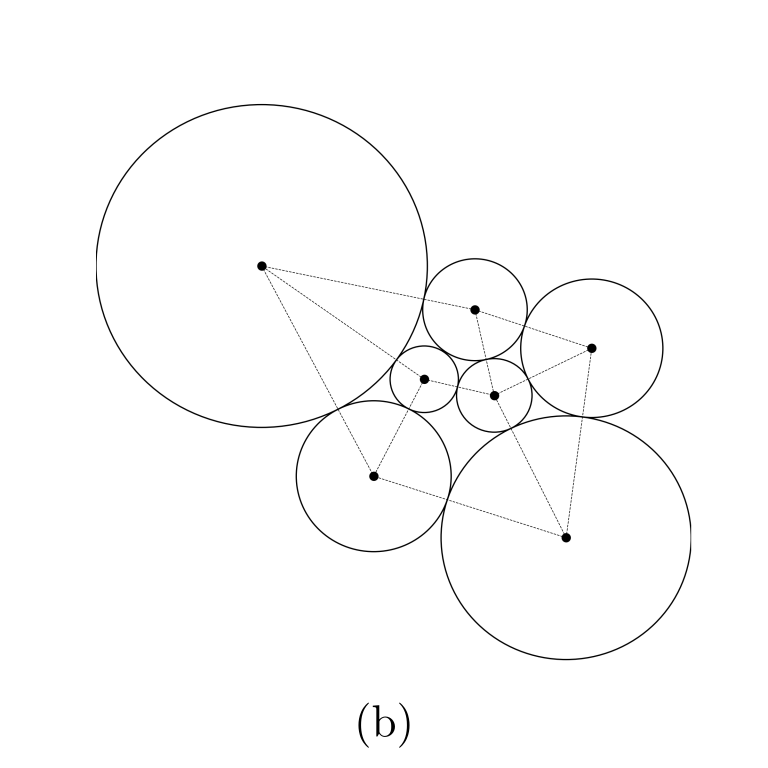
\includegraphics[width = 0.4\textwidth]{Chapter 1/packing_contact.png}   
    \end{tabular}
    \caption{(a) A circle packing with 7 circles. (b) The packing with its contact graph visualized.}
\end{figure}
\vspace{-2 mm}
\begin{flushleft}
One such property, and the main focus of this project, is \textit{rigidity}, which was first studied by James Clerk Maxwell. Rigidity is a measure of how `stiff' something is, and can be seen when we consider structures such as buildings, bridges, sandcastles and so on. Some of them hold up, whereas others don't. This is partly due to the material it is made from, and also because of the fact that some of these structures are rigid, while others are not.     
\end{flushleft}

\begin{flushleft}
In this project, we will be introduced to the ideas of rigidity, what it means for a \textit{framework} to be rigid, and how we can study the rigidity of circle packings. Along the way, we will try to gain some insight to the conjecture that this thesis focuses on:

\begin{center}
    \textit{``For every planar and minimally rigid graph, does there exist a circle packing that is also infinitesimally rigid?''}
\end{center}
\end{flushleft}

\noindent
where the terms stated in this question will be defined in due time.

\begin{flushleft}
An exciting aspect of this project is the way in which various fields within mathematics become involved when studying something that seems purely geometric. Ideas from Graph Theory and Linear Algebra come into play and therefore, the intended audience for this project are mathematics students that are accustomed to these two fields, as well as a basic understanding of how to code. That being said however, everything will be clearly defined and explained as we come across it. Moreover, all the code involved in this project can be viewed on Github at \href{https://github.com/Titwik/Dissertation}{Titwik/Dissertation}.    
\end{flushleft}

\begin{flushleft}
The only pre-requisite required to understand the content of this project involves some fundamental linear algebra. Specifically, the knowledge of how vectors work, and a good understanding of matrices and their properties. The interested reader can explore the flavor of mathematics involved in this project in texts relating to;
\begin{itemize}
    \item \textit{Graph Theory}: The study of mathematical structures, known as graphs, that represent relationships between objects. It has several applications, some of which include computer science, biology and logistics to name a few.
    \item \textit{Discrete Mathematics}: The study of countable, discrete objects rather than continuous quantities. Topics involved include Set Theory and Logic, and it plays a big role in the study of computer science.
    \item \textit{Constrained Optimization}: Attempting to find the maximum or minimum of a certain `objective' function while adhering to specific constraints. 
\end{itemize}
\end{flushleft}

\begin{flushleft}
With all that said, let's get started!
\end{flushleft}



\clearpage

%----------------------------------------------------------------------

\chapter{Rigidity: An Introduction} % previously Definitions \& Preliminaries

\begin{flushleft}
Rigidity can be easily understood as observing a structure and questioning how 'stiff' it is. If some force is applied to it, does it bend or buckle? When we pull the structure across (Euclidean) space, do we move it entirely, or does a part of it bend and move in the direction of the pull? As stiffness can be interpreted in a multitude of ways, this chapter will be dedicated to formalizing the definition of rigidity that we will use for the remainder of this project. 
\end{flushleft}

\begin{flushleft}
To start, we must first understand what \textit{graphs} are.
\end{flushleft}

\section{Graph Theory}

\begin{flushleft}
Here, we delve into a small portion of a very large field of mathematics. The definitions presented here will be fundamental for what's to come.
\end{flushleft}

\begin{definition}
    A \textit{graph} $G = (V,E)$ consists of a set V and a set E of two-element subsets of V. The elements of V are called \textit{vertices} (or nodes) and the elements of E are called \textit{edges}.
\end{definition}

\begin{example}
The graph $G = (V,E)$ below
\label{eg: cycle}
\begin{figure}[ht]
    \centering
    \documentclass{standalone}
\usepackage{tikz}
\usetikzlibrary{arrows,backgrounds,positioning,petri, calc}


\begin{document}
% Set the style for the vertices
\tikzstyle{vertex} = [circle, draw=black, fill = black, thin, inner sep=0pt,minimum size=2mm]

\begin{tikzpicture}
    
    % Define nodes
    \node (1) at (0,0) [vertex, label=left:$1$] {};
    \node (2) at (1,1) [vertex, label=above:$2$] {};
    \node (3) at (2.5,1) [vertex, label=above:$3$] {};
    \node (4) at (2.5,-1) [vertex, label=below:$4$] {};
    \node (5) at (1,-1) [vertex, label=below:$5$] {};

    % add edges
    \path[] (1) edge (2)
                edge (5)
            (3) edge (2)
                edge (4)
            (4) edge (5);
    
\end{tikzpicture}
\end{document}

% when entering figures, use the following format

%\begin{figure}[htbp]
%    \centering
%    \input{Chapter 1/framework}
%    \caption{Caption}
%    \label{fig:enter-label}
%\end{figure}
    \label{simple graph}
\end{figure}
\noindent
has $|V| = 5$, and $|E| = 5$.
\end{example}

\begin{definition}
A graph $G$ is \textit{connected} if for any two vertices $u,v$, there exists a sequence of distinct vertices (called a \textit{path}) $u_1, \hdots, u_k$, such that $u_iu_{i+1}$ is an edge of $G$ for $0 \leq i \leq k-1$ that connect $u$ and $v$. The path can be seen as 

\[
u = u_0, u_1, \hdots, u_{k-1}, u_k = v
\]
\end{definition}

\begin{definition}
A \textit{cycle} is a graph $G = (V,E)$  where $G$ has $n$ vertices, and the edges are 

\[
E(G) = \{12, 23, \hdots, (n-1)n \}
\]

\noindent
It can be thought of as a closed path. 
\end{definition}

\begin{example}
The graph in Example \ref{eg: cycle} is a cycle of length 5.
\end{example}

\begin{definition}
The \textit{degree} of a vertex is the number of edges incident to the vertex.
\end{definition}

\begin{flushleft}
There are several ways of drawing the 'same' graph on the plane. This includes labelling them in a variety of ways as well. Therefore, it is vital that we class these drawings as the same graph.
\end{flushleft}

\begin{definition}
\label{def: isomorphism}
Two graphs $G_1$ and $G_2$ are said to be \textit{isomorphic} if there is a bijection $\phi$ : $V(G_1) \rightarrow V(G_2)$ such that $xy \in E(G_1)$ if and only if $\phi(x)\phi(y) \in E(G_2)$. The function $\phi$ is known as an \textit{isomorphism}.
\end{definition}

\begin{example}
\label{eg: isomorphic graphs}
Consider the two graphs below.

\begin{figure}[ht]
    \centering
    \documentclass{standalone}
\usepackage{tikz}
\usetikzlibrary{arrows,backgrounds,positioning,petri, calc}


\begin{document}
% Set the style for the vertices
\tikzstyle{vertex} = [circle, draw=black, fill = black, thin, inner sep=0pt,minimum size=2mm]

\begin{tikzpicture}
    
    % Define nodes for the first K4
    \node (11) at (0,0) [vertex, label=below:$1$] {};
    \node (12) at (0,2) [vertex, label=above:$2$] {};
    \node (13) at (2,2) [vertex, label=above:$3$] {};
    \node (14) at (2,0) [vertex, label=below:$4$] {};
    \node[draw = none] (G1) at (1,-1) [label=above:$G_1$] {};

    % define nodes for the second K4
    \node (21) at (4,0) [vertex, label=below:$a$] {};
    \node (22) at (4,2) [vertex, label=above:$b$] {};
    \node (23) at (6,2) [vertex, label=above:$c$] {};
    \node (24) at (6,0) [vertex, label=below:$d$] {};
    \node[draw = none] (G1) at (5,-1) [label=above:$G_2$] {};

    % add the edges
    \path[] (11) edge (12)
                edge (14)
            (12) edge (13)
            (13) edge (11); 

    \path[] (21) edge (23)
            (22) edge (23)
                edge (24)
            (23) edge (24);
\end{tikzpicture}
\end{document}
    %\caption{Caption}
    \label{fig:isomoprhic graphs}
\end{figure}
\vspace{-5 mm}
\begin{flushleft}
The bijection $\phi : G_1 \rightarrow G_2$ is given by $\phi(1) = c$, $\phi(2) = b$, $\phi(3) = c$, and $\phi(4) = a$.    
\end{flushleft}
\end{example}

\begin{flushleft}
Given a graph $G$, we may be interested in a certain subset of vertices and edges that are included in $G$. This involves studying a \textit{subgraph} of $G$.
\end{flushleft}

\begin{definition}
A graph $H$ is a \textit{subgraph} of $G$ if there is a graph $H'$ isomorphic to $H$ such that $V(H') \subseteq V(G)$ and $E(H') \subseteq E(G)$.
\end{definition}

\begin{example}
Consider the graphs below.

\begin{figure}[ht]
    \centering
    \documentclass{standalone}
\usepackage{tikz}
\usetikzlibrary{arrows,backgrounds,positioning,petri, calc}


\begin{document}
% Set the style for the vertices
\tikzstyle{vertex} = [circle, draw=black, fill = black, thin, inner sep=0pt,minimum size=2mm]

\begin{tikzpicture}
    
    % Define nodes
    \node (1) at (0,0) [vertex, label=left:$1$] {};
    \node (2) at (1,1) [vertex, label=above:$2$] {};
    \node (3) at (3,1) [vertex, label=above:$3$] {};
    \node (4) at (3,-1) [vertex, label=below:$4$] {};
    \node (5) at (1,-1) [vertex, label=below:$5$] {};
    \node[draw = none] (G1) at (2,-2.25) [label=above:$G$] {};

    \node (21) at (6,0) [vertex, label=left:$1$] {};
    \node (22) at (7,1) [vertex, label=above:$2$] {};
    \node (25) at (7,-1) [vertex, label=below:$5$] {};
    \node[draw = none] (H) at (7,-2.25) [label=above:$H$] {};
    

    % add edges
    \path[] (1) edge (2)
                edge (5)
            (3) edge (2)
                edge (4)
            (4) edge (5)
            (2) edge (5)
            (21) edge (22)
                edge (25)
            (22) edge (25);
    
\end{tikzpicture}
\end{document}

    %\caption{Caption}
    %\label{fig:enter-label}
\end{figure}
\noindent
Here, as $V(H) \subseteq V(G)$ and $E(H) \subseteq E(G)$, it follows that $H$ is a subgraph of $G$.
\end{example}

\begin{flushleft}
The last idea we need from graph theory is the notion of \textit{planarity}. The graphs we are interested in for this project are those such that the edges do not cross over each other.
\end{flushleft}

\begin{definition}
    \label{def: planar graphs}
    A graph $G$ is \textit{planar} if it has a drawing in the plane such that none of edges cross over each other.
\end{definition}

\begin{example}
    Consider \hyperref[eg: isomorphic graphs]{Example \ref*{eg: isomorphic graphs}}. The graph $G_1$ is a planar drawing of the graph $G_2$.
\end{example}

\section{Frameworks}

\begin{flushleft}
    Now that we have a good idea of what graphs are, we can start working on setting up frameworks. The definitions in this section will be defined in the space $\mathbb{R}^d$, where $d \in \mathbb{N}$. Later, we will find ourselves working exclusively in $\mathbb{R}^2$. For the remainder of this chapter, we shall adhere closely to the contents in chapter 2 from the book ``Frameworks, Tensegrities, and Symmetry'' by Robert Connelly and Simon D. Guest \cite{textbook}.
\end{flushleft}

\noindent
The first definition we need is that of a \textit{configuration}.

\begin{definition}
    Suppose we have a collection of $n$ labelled points in $\mathbb{R}^d$, where $d \in \mathbb{N}$. Let $\mathbf{p}_i = (p_{i1}, \hdots, p_{id})$ be the position vector of point $i$. Then a \textit{configuration} is

\[
\mathbf{p} = (\mathbf{p}_1, \hdots, \mathbf{p}_n),
\]

\begin{flushleft}
where $\mathbf{p}$ is a vector of vectors in $\mathbb{R}^d$.     
\end{flushleft}
\end{definition}

\begin{flushleft}
Therefore, a configuration can be thought of as a set of points in the space $\mathbb{R}^d$, each point equipped with its own position vector. Henceforth, we will refer the the points in a configuration as \textit{nodes}. 
\end{flushleft}

\begin{flushleft}
Given a configuration, we can now decide which pairs of nodes to connect with a graph $G$. The nodes in $\mathbf{p}$ correspond to the vertices in $G$, and $G$ is not allowed to have multiple edges between vertices, or loops between the same vertex (such graphs are known to be \textit{simple}).
\end{flushleft}

\begin{definition}
    A \textit{framework} is a configuration $\mathbf{p} = (\mathbf{p}_1, \hdots, \mathbf{p}_n)$ together with its corresponding graph $G = (V,E)$. We denote it as $(G,\mathbf{p})$.
\end{definition}

%** IS THIS NEEDED?
\begin{flushleft}
Note that as we are working in $\mathbb{R}^d$, the \textit{length} of each edge with endpoints $\mathbf{p}_i$ and $\mathbf{p}_j$ in a framework $(G,\mathbf{p})$ is the \textit{Euclidean distance} between the points $\mathbf{p}_i$ and $\mathbf{p}_j$. This is denoted $|\mathbf{p}_i - \mathbf{p}_j|$.

In this project, graphs will be drawn with vertices that are filled in, whereas frameworks will have hollow nodes. 
\end{flushleft}

%\clearpage

\begin{example}
\label{g vs f}
In the two diagrams below, the one on the left is a graph, whereas the one on the right is a framework.
    \begin{figure}[h]
        \centering
        \documentclass{standalone}
\usepackage{tikz}
\usetikzlibrary{arrows,backgrounds,positioning,petri, calc}


\begin{document}
% Set the style for the vertices
\tikzstyle{vertex} = [circle, draw=black, thin, inner sep=0pt,minimum size=2mm]

\begin{tikzpicture}
    
    % Define nodes for the first K4
    \node (11) at (0,0) [vertex, fill = black] {};
    \node (12) at (0,2) [vertex, fill = black] {};
    \node (13) at (2,2) [vertex, fill = black] {};
    \node (14) at (2,0) [vertex, fill = black] {};

    % add invisible node at (1,-1)
    \node[draw = none] (graph) at (1, -.5) {Graph};

    % define nodes for the second K4
    \node (21) at (4,0) [vertex] {};
    \node (22) at (4,2) [vertex] {};
    \node (23) at (6,2) [vertex] {};
    \node (24) at (6,0) [vertex] {};

    \node[draw = none] (graph) at (5, -.5) {Framework};

    % add the edges
    \path[] (11) edge (12)
                edge (14)
            (12) edge (13)
            (13) edge (11)
                edge (14); 

    \path[] (21) edge (22)
                edge (24)
            (22) edge (23)
            (23) edge (21)
                edge (24); 
\end{tikzpicture}
\end{document}
    \end{figure}
\end{example}
\vspace{-8 mm}
\begin{flushleft}
At this stage, you may be wondering what exactly the difference between a graph and a framework is. Put simply,
\begin{itemize}
    \item A graph is an abstract mathematical object that can be visualised in a multitude of ways, as seen in \hyperref[eg: isomorphic graphs]{Example \ref*{eg: isomorphic graphs}}. Varying the edge lengths does not produce a new graph as by \hyperref[def: isomorphism]{Definition \ref*{def: isomorphism}}, they are isomorphic, and considered the `same'.
    \vspace{-3mm}
    \item In a framework however, each node has a position vector. If we consider a framework in $\mathbb{R}^2$ such as the one in \hyperref[g vs f]{Example \ref*{g vs f}}, each node is at a determined distance from each other. Slightly changing the position of a node results in a different framework.

\end{itemize}
\end{flushleft}

\begin{flushleft}
Frameworks are essential when it comes to studying the rigidity of structures. Considering real-world applications, a simple model of a building can be designed by considering what its framework would look like in $\mathbb{R}^3$. Investigating this framework allows for insight into how the building in question should be built.
\end{flushleft}

\noindent
Armed with the notion of a framework, we can begin thinking about how we might be able to change the shape of a framework. 

\section{Motions}

\begin{flushleft}
When it comes to studying the rigidity of frameworks, we begin by understanding what it means for a framework to experience a \textit{motion} (also known as a \textit{flex}). 
\end{flushleft}

\begin{definition}
Suppose the configuration $\mathbf{p} \in \mathbb{R}^d$ is on a differentiable smooth path parameterized by time $t$, denoted $\mathbf{p}(t)$. Then 

    \begin{itemize}
        \item The position of node $\mathbf{p}_i \in \mathbf{p}$ at any time $t$ is given by $\mathbf{p}_i(t) \in \mathbb{R}^d$.
        \vspace{-3mm}
        \item The \textit{initial position} of a node $\mathbf{p}_i$ is $\mathbf{p}_i(0) \in \mathbb{R}^d$
        \vspace{-3mm}
        \item The \textit{initial configuration} of $\mathbf{p}$ is 
        \[
        \mathbf{p}(0) = (\mathbf{p}_1(0), \hdots, \mathbf{p}_n(0) \in \mathbb{R}^{nd}
        \]
    \end{itemize}
\end{definition}

\begin{definition}
A \textit{motion} of the framework $(G,\mathbf{p})$ is a path $\mathbf{p}(t)$ such that 

\[
|\mathbf{p}_i(t) - \mathbf{p}_j(t)| = |\mathbf{p}_i(0) - \mathbf{p}_j(0)|,
\]

\noindent
for all $t$, and for all $ij \in E(G)$.
\end{definition}

\begin{flushleft}
In other words, a motion preserves the length of every edge in the framework at any point in time. A motion $\mathbf{p}(t) = (\mathbf{p}_1(t), \hdots, \mathbf{p}_n(t))$ is a \textit{continuous motion} if each of the $d$ coordinates of $\mathbf{p}_i(t)$ is continuous in $t$. This simply means that the nodes of the configuration should follow an uninterrupted path in $\mathbb{R}^d$ with respect to time. 
\end{flushleft}

\begin{flushleft}
There are certain motions that we can apply to a framework such that the distances between all the nodes are preserved as well. Such motions are known as \textit{rigid motions}.
\end{flushleft}

\begin{definition}
A \textit{rigid motion} of the framework $(G,\mathbf{p})$ is a path $\mathbf{p}(t)$ such that 

\[
|\mathbf{p}_i(t) - \mathbf{p}_j(t)| = |\mathbf{p}_i(0) - \mathbf{p}_j(0)|,
\]

\noindent
for all $t$, and for all $i, j \in V(G)$
\end{definition}

\begin{flushleft}
From this definition, we can see that there are only two ways in which a motion can be classed as a rigid motion.     
\end{flushleft}

\begin{itemize}
    \item \textit{Translating} the entire framework across $\mathbb{R}^d$ preserves the distances between each node, and so it is a rigid motion.
    \vspace{-3mm}
    \item \textit{Rotating} the entire framework about a point also preserves the distances between each node. Thus, it is a rigid motion as well.
    
\end{itemize}

\begin{flushleft}
In order to formalize this, we let the matrix $\mathbf{Q}(t)$ describe a rotation of a node in $\mathbb{R}^d$, where $\mathbf{Q}(0)$ is the identity matrix, and we let $\mathbf{w}(t)$ be a translation of a node in $\mathbb{R}^d$, where $\mathbf{w}(0)$ is the zero vector. Then we can classify all rigid motions as paths of each node $\mathbf{p}_i(t)$ that have the form 

\[
\mathbf{p}_i(t) = \mathbf{Q}(t)\mathbf{p}_i + \mathbf{w}(t)
\]

\vspace{2mm}
Thus, rotating and translating a framework in any combination is always a rigid motion.
\end{flushleft}

\begin{example}
\label{eg: simple motion}
Consider the framework with three nodes, labelled $1,2,3$, and two edges, $12$, and $23$. Apply the motion 

\[ p_i(t) = 
\begin{cases}
    \cos(t) - \sin(t), & \text{if } i = 3 \\
    p_i(0), & \text{if } i = 1,2
\end{cases}
\]

\vspace{3 mm}
\noindent
to this framework. A diagram of what happens for times $t=0$, and $t=1$ is shown below
%\clearpage

    \begin{figure}[htbp]
        \centering
        \documentclass{standalone}
\usepackage{tikz}
\usetikzlibrary{arrows,backgrounds,positioning,petri, calc}

\begin{document}
% Set the style for the vertices
\tikzstyle{vertex} = [circle, draw=black, thin, inner sep=0pt,minimum size=2mm]

\begin{tikzpicture}

    % before the motion
    \node (11) at (0,0) [vertex, label=above:$\textbf{p}_1$] {};
    \node (12) at (2,0) [vertex, label=above:$\textbf{p}_2$] {};
    \node (13) at (2,-2) [vertex, label=below:$\textbf{p}_3$] {};

    \node[draw = none] (t1) at (-0.2, -1.5) {$t = 0$};
    %\draw[->] (2.5,-1) -- (4.5,-1);
    % after the motion
    \node (21) at (5,0) [vertex, label=above:$\textbf{p}_1$] {};
    \node (22) at (7,0) [vertex, label=above:$\textbf{p}_2$] {};
    \node (23) at (5.6, -1.4) [vertex, label = below: $\textbf{p}_3$] {};

    \node[draw = none] (t2) at (4.5, -1) {$t = 1$};

    % add the edges before the motion
    \path[] (11) edge (12);
    \path[] (12) edge (13); % Make this edge red
    
    % Swing node (13) along an arc towards node (11)
    \path[draw, ->, dashed] (13) edge [bend left = 40] (11); 

    % add the edges before the motion
    \path[] (21) edge (22);
    \path[] (22) edge (23); % Make this edge red
    
    % Swing node (13) along an arc towards node (11)
    \path[draw, ->, dashed] (23) edge [bend left = 20] (21); 

\end{tikzpicture}
\end{document}

        \caption{A framework where the edge $23$ can swing about $2$.}
        \label{fig: simple motion}
    \end{figure}
\vspace{-5 mm}
\begin{flushleft}
As all the edge lengths are preserved, this is a motion. However, the distance between nodes $1$ and $3$ changes as $t$ changes. Therefore, this is not a rigid motion.    
\end{flushleft}
\end{example}

\begin{example}
Consider the matrix 

\[ \mathbf{Q} = 
\begin{pmatrix}
-1 & 0\\
0 & -1\\
\end{pmatrix}
\]

\begin{flushleft}
This results in a rotation of each node by 180$\degree$ about the origin $O$ in $\mathbb{R}^2$. Applying this to a framework at $t = 0$ in \hyperref[eg: simple motion]{Example \ref*{eg: simple motion}}, we obtain

\begin{figure}[htbp]
    \centering
    \documentclass{standalone}
\usepackage{tikz}
\usepackage{gensymb}
\usetikzlibrary{arrows,backgrounds,positioning,petri, calc}

\begin{document}
% Set the style for the vertices
\tikzstyle{vertex} = [circle, draw=black, thin, inner sep=0pt,minimum size=2mm]

\begin{tikzpicture}[node distance = 2cm, auto, scale = 1]

    %\tikzstyle{every node}=[font=\small]

    % before the motion
    \node (11) at (-1,0) [vertex, label=above:$\textbf{p}_1$] {};
    \node (12) at (1,0) [vertex, label=above:$\textbf{p}_2$] {};
    \node (13) at (1,-2) [vertex, label=below:$\textbf{p}_3$] {};

    % add node for the origin
    \node (origin) at (0,-1) [vertex, fill = black, label=below:$O$] {};

    % add an invisble node
    \node[draw = none] (start) at (1.2, -1) {};

    % add an invisible node for the label
    \node[draw = none] (label) at (3.5, -1)[label=above:Multiply by $\mathbf{Q}$]{};

    % after the motion
    \node (21) at (8,-2) [vertex, label=below:$\textbf{p}_1$] {};
    \node (22) at (6,-2) [vertex, label=below:$\textbf{p}_2$] {};
    \node (23) at (6, 0) [vertex, label = above: $\textbf{p}_3$] {};

    % add node for the origin
    \node (origin2) at (7, -1) [vertex, label = above: $O$, fill = black] {};

    % add an invisble node
    \node[draw = none] (end) at (5.8, -1) {};

    % add the edges before the motion
    \path[] (11) edge (12);
    \path[] (12) edge (13); % Make this edge red
    
    % add the edges before the motion
    \path[] (21) edge (22);
    \path[] (22) edge (23);  

    % plot the line between the diagrams
    \draw[->] (start) -- (end);
    

\end{tikzpicture}
\end{document}

\end{figure}

As all the edge lengths, as well as the distances between each node are preserved, this is a rigid motion.    
\end{flushleft}
\end{example}

\section{Rigidity}
\begin{flushleft}
As we have seen, rigid motions maintain not only the lengths of every edge in a framework, but they also fix the distance between each node as well. At this stage, we can question what frameworks can only be subject to rigid motions. Is there a framework such that the only way to move it is if we move \textit{all} of it?

The answer is yes, and such frameworks are said to be \textit{rigid}.
\end{flushleft}

\begin{definition}
\label{def: rigid}
A framework $(G,\mathbf{p})$ is rigid if every continuous motion $\mathbf{p}(t) = (\mathbf{p}_1(t), \hdots, \mathbf{p}_n(t))$ is a rigid motion. 
If a framework is not rigid, it is said to be \textit{flexible}.
\end{definition}

\begin{example}
\label{eg: rigid graphs}    
The frameworks in Figure \ref{fig: rigid_graphs} are rigid. 

\vspace{3mm}
\begin{figure}[htbp]
    \centering
    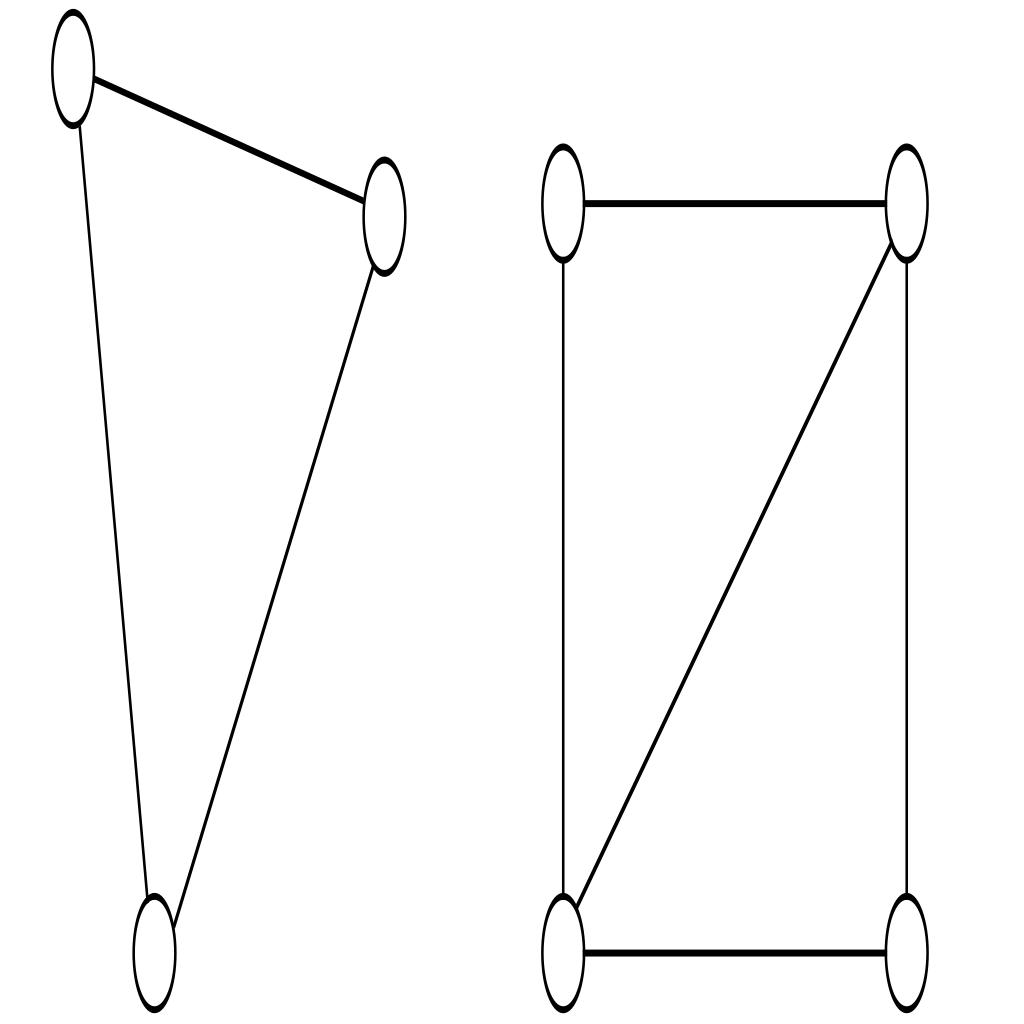
\includegraphics[width=0.57\textwidth]{Chapter 2/7. rigid_graphs.png} 
    \caption{Two rigid frameworks in $\mathbb{R}^2$}
    \label{fig: rigid_graphs}
\end{figure}

\begin{flushleft}
However, the framework in Figure \ref{eg: not_rigid} is not. We can apply a motion to the two nodes at the top such that the edge lengths are preserved, but the distance between the diagonal nodes change, violating the definition of rigidity.    
\end{flushleft}

\begin{figure}[htbp]
    \centering
    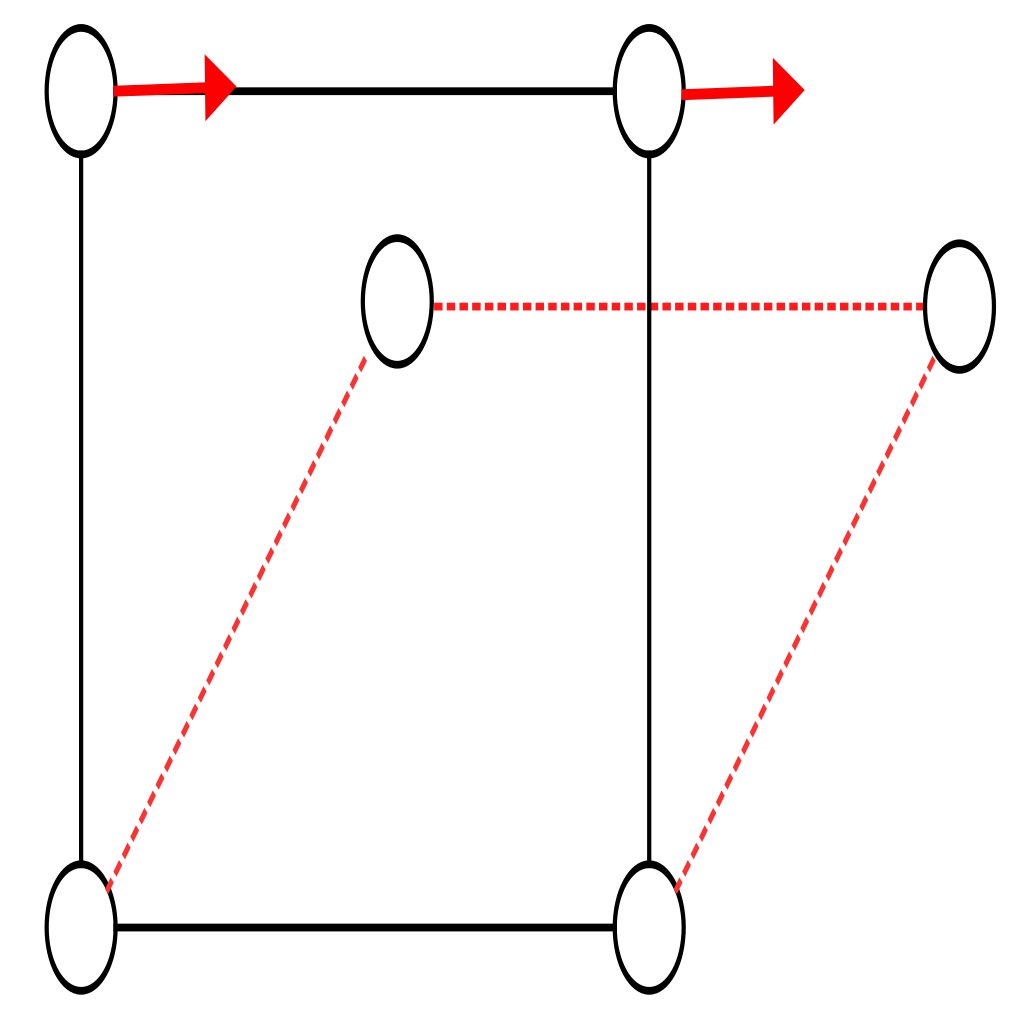
\includegraphics[width = 0.4\textwidth]{Chapter 2/8. not_rigid.png}
    \caption{A framework that is not rigid in $\mathbb{R}^2$}
    \label{eg: not_rigid}
\end{figure}
\end{example}
\vspace{-5 mm}
\begin{flushleft}

\vspace{-3mm}
Another equivalent definition that was proved by Asimow and Roth \cite{asimow} that uses ideas of the congruency of frameworks.
\end{flushleft}

\begin{definition}
Consider two frameworks $(G,\mathbf{p})$ and $(G,\mathbf{q})$ where $\mathbf{p} = (\mathbf{p}_1, \hdots, \mathbf{p}_n)$ and $\mathbf{q} = (\mathbf{q}_1, \hdots, \mathbf{q}_n)$.
\begin{itemize}
    \item $\mathbf{q}$ is \textit{equivalent} to $\mathbf{p}$ if $|\mathbf{p}_i - \mathbf{p}_j| = |\mathbf{q}_i - \mathbf{q}_j|$ for all $ij \in E(G)$.
    \vspace{-3mm}
    \item $\mathbf{q}$ is \textit{congruent} to $\mathbf{p}$ if $|\mathbf{p}_i - \mathbf{p}_j| = |\mathbf{q}_i - \mathbf{q}_j|$ for all $i, j \in V(G)$.
\end{itemize}
\end{definition}

\begin{flushleft}
To put it another way, two frameworks $(G,\mathbf{p})$ and $(G,\mathbf{q})$ are equivalent if the edge lengths are the same for every pair of labelled nodes in $(G,\mathbf{p})$.

They are congruent if $(G,\mathbf{p})$ can be obtained through a series of rotations and translations of $(G,\mathbf{q})$. 
\end{flushleft}

% https://www.youtube.com/watch?v=kQlrqrjBXtk, 3:03
\begin{definition}
A framework $(G,\mathbf{p})$ on $n$ nodes is \textit{rigid} if there exists an $\epsilon>0$ such that for every configuration $\mathbf{q}$, where $(G,\mathbf{q})$ is equivalent to $(G,\mathbf{p})$, satisfies 

\[
|\mathbf{p}_i - \mathbf{q}_i| < \epsilon
\]
\begin{flushleft}
for all $i \in V(G)$, and is congruent to $(G,\mathbf{p})$.  
\end{flushleft}
\end{definition}

\begin{figure}[htbp]
    \centering
    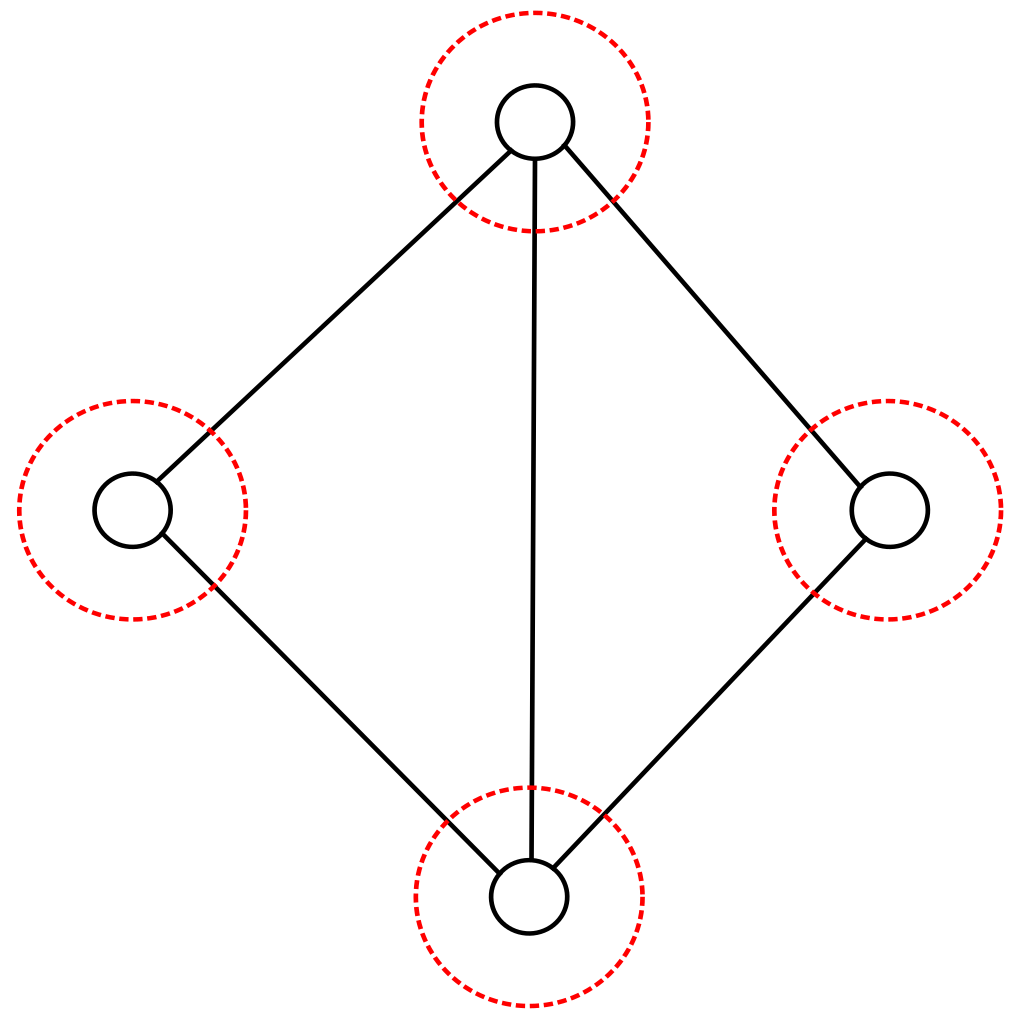
\includegraphics[width = 0.35\textwidth]{Chapter 2/14. epsilon.png}
    \caption{A framework $\mathbf{p}$ with an epsilon bound (red) for every node}
    \label{fig: epsilon}
\end{figure}
\vspace{-3mm}
\begin{flushleft}
In Figure \ref{fig: epsilon}, we visualise what an epsilon bound for every node looks like. If we create a configuration $\mathbf{q}$ such that it is equivalent to the framework $\mathbf{p}$ in the figure, and the nodes of $\mathbf{q}$ fall within the epsilon bounds of each node in $\mathbf{p}$, then we are able to conclude that with some rigid motion, we are able to achieve congruence between $\mathbf{p}$ and $\mathbf{q}$. 

In such scenarios, equivalence implies congruence.    
\end{flushleft}

% https://www.youtube.com/watch?v=kQlrqrjBXtk
% 8:30
\subsection{Infinitesimal Rigidity}

\begin{flushleft}
In some sense, the definition of rigidity seems quite loose. Depending on the material used to construct the edges of the framework, we may be able to deform the edges. 
\end{flushleft}

\begin{figure}[htbp]
    \centering
    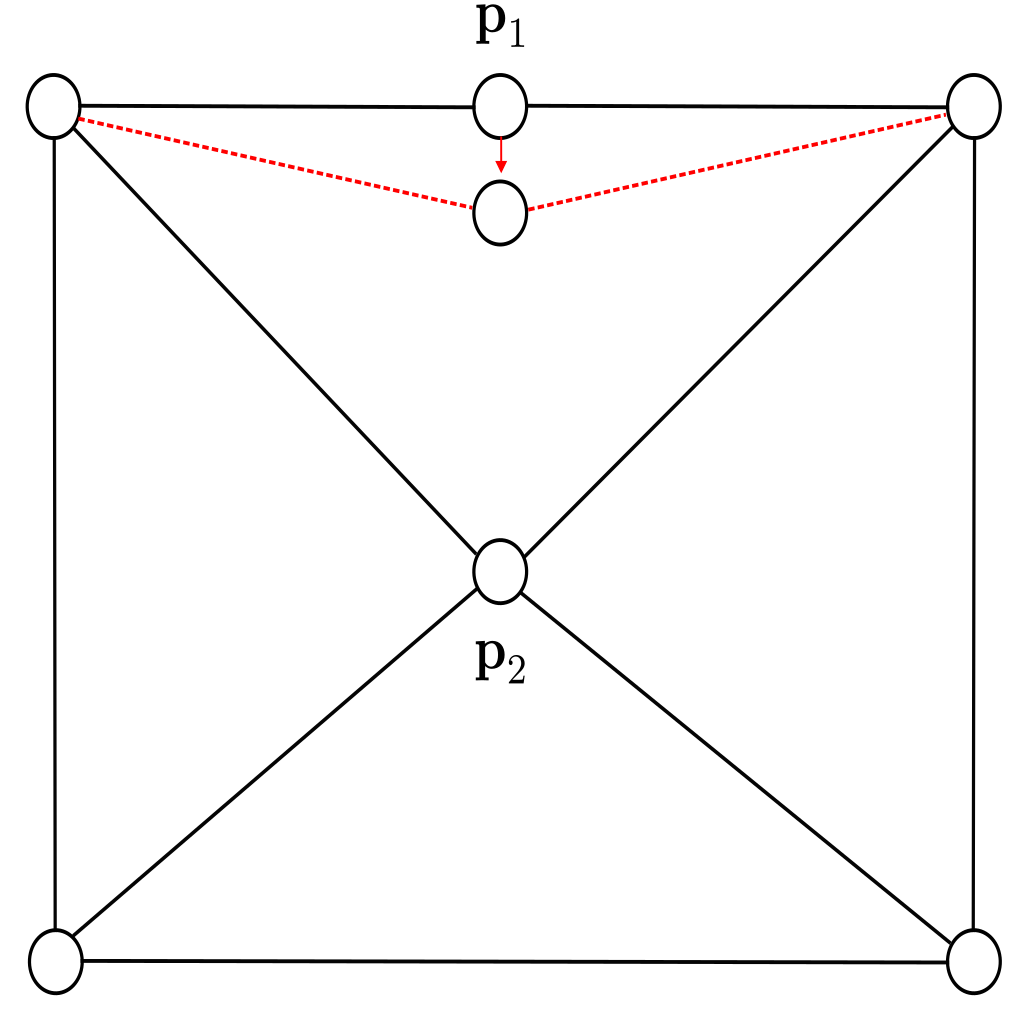
\includegraphics[width = 0.32\textwidth]{Chapter 2/9. not_inf_rigid.png}
    \caption{A framework with all nodes pinned, and an edge that can be displaced.}
    \label{fig: not_inf_rigid}
\end{figure}
\vspace{-2 mm}
\begin{flushleft}
Looking at Figure \ref{fig: not_inf_rigid}, if we consider the dotted edge to be a piece of string tied between two fixed nodes, then we can apply some force and deform the structure. Although the initial framework is rigid, it somehow doesn't `feel' rigid.
\end{flushleft}

\begin{flushleft}
In order to strengthen the definition of rigidity, let us first start with an observation described in greater detail by Graver in his book ``Counting on Frameworks'' \cite{counting_frameworks}. 
\end{flushleft}

\begin{flushleft}
Suppose that the configuration $\mathbf{p}$ is on a smooth differentiable path parameterized by time $t$. Consider a node of the configuration $\mathbf{p}_i$. Then its position is given by $\mathbf{p}_i(t)$ and as $\mathbf{p}_i$ is on a differentiable path, its derivative is well-defined.
\end{flushleft}

\begin{figure}[htbp]
    \centering
    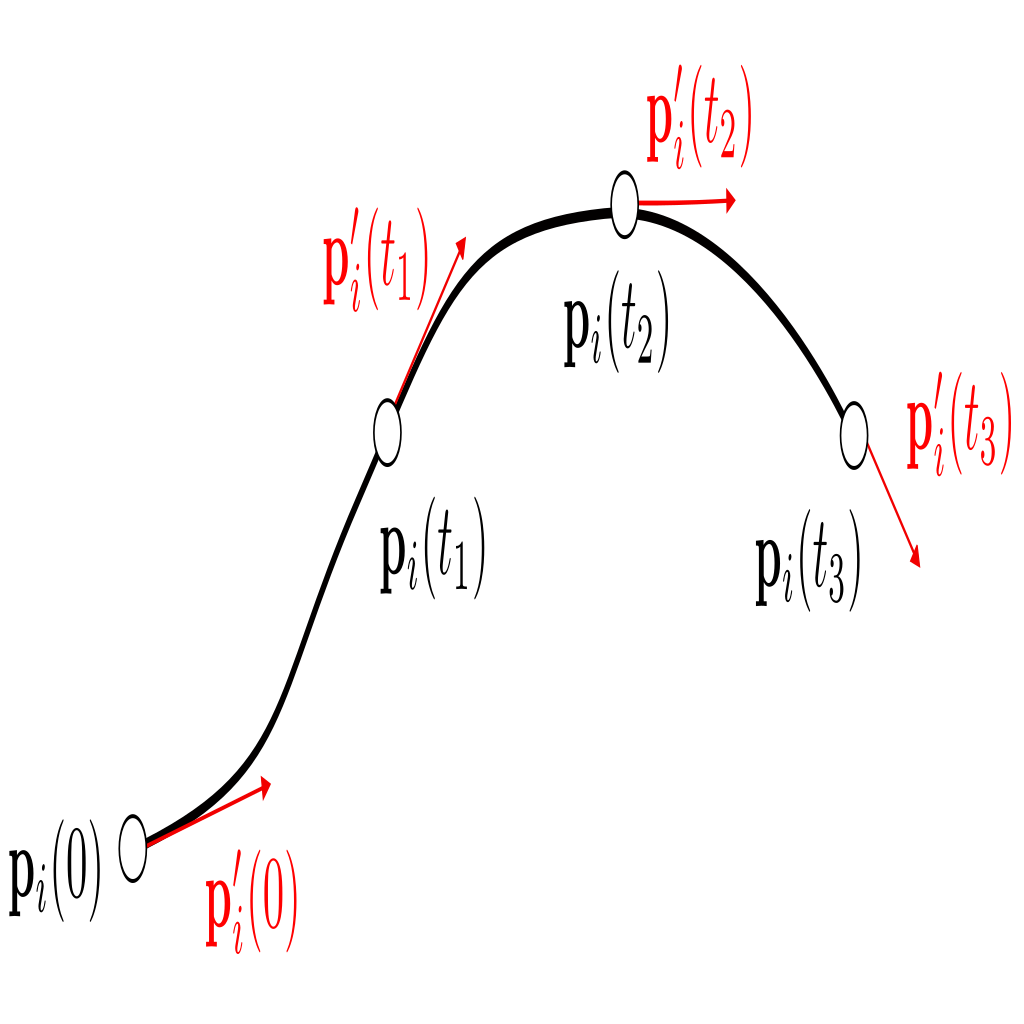
\includegraphics[width = 0.5\textwidth]{Chapter 2/12. path.png}
    \caption{Node $\mathbf{p}_i$ at various positions on path $\mathbf{p}_i(t)$ for various times $t$. The instantaneous velocities at each position $\mathbf{p}'_i(t)$ are marked in red}
    \label{fig: path}
\end{figure}

\vspace{-3mm}
\begin{flushleft}
    Taking the derivative of $\mathbf{p}_i(t)$ with respect to time gives us the instantaneous velocity $\mathbf{p}'_i(t)$ of the node $\mathbf{p}_i$ at time $t$.    
\end{flushleft}

%\vspace{-5.5 mm}

\begin{flushleft}
The velocities $\mathbf{p}'_i(t)$ become vital when studying infinitesimal rigidity. To motivate this, let us consider a framework in $\mathbb{R}^2$.
\end{flushleft}

\begin{figure}[htbp]
    \centering
    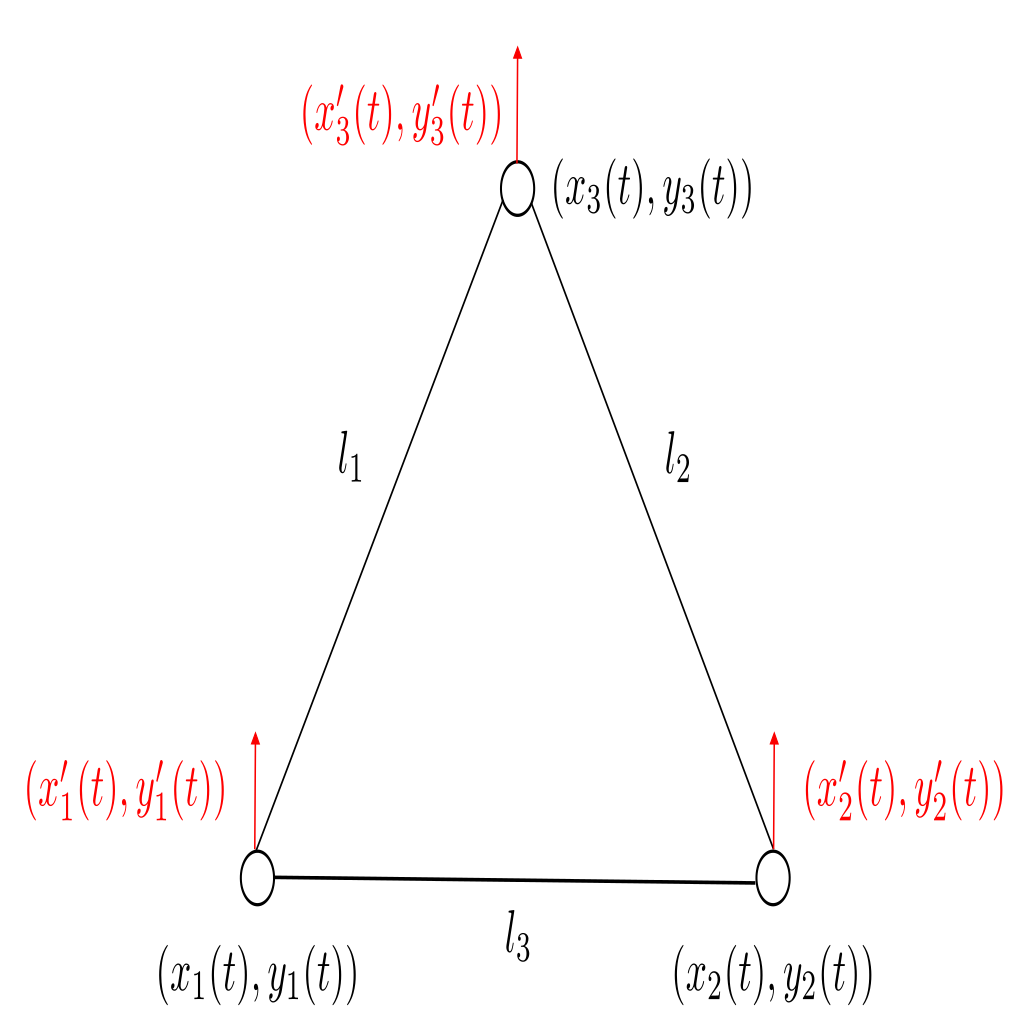
\includegraphics[width = 0.65\textwidth]{Chapter 2/13. inf_rigid_proof.png}
    \caption{A framework in $\mathbb{R}^2$, with some instantaneous velocity vectors at each node given in red.}
    \label{fig: inf_velocity}
\end{figure}

\vspace{-3mm}
\begin{flushleft}
In Figure \ref{fig: inf_velocity}, we have a framework with three nodes, each defined by coordinates $(x_i(t), y_i(t))$ as well as their corresponding velocities given by $(x'_i(t), y'_i(t))$ for $i = 1,2,3$. As each point is fixed in the plane, the distances between each pair of nodes are constants, given as $l_i$ for $i = 1,2,3$.
\end{flushleft}

\begin{flushleft}
Therefore, we know that 
%\vspace{-1 mm}
\[
\begin{split}
(x_1(t) - x_2(t))^2 + (y_1(t) - y_2(t))^2 = {l_3}^2 \\
(x_1(t) - x_3(t))^2 + (y_1(t) - y_3(t))^2 = {l_1}^2 \\
(x_2(t) - x_3(t))^2 + (y_2(t) - y_3(t))^2 = {l_2}^2
\end{split}
\]

Now, if we differentiate each equation with respect to $t$, we get 
%\vspace{-1 mm}
\[
\begin{split}
2(x_1 - x_2)(x'_1 - x'_2) + 2(y_1 - y_2)(y'_1 - y'_2) = 0 \\
2(x_1 - x_3)(x'_1 - x'_3) + 2(y_1 - y_3)(y'_1 - y'_3) = 0 \\
2(x_2 - x_3)(x'_2 - x'_3) + 2(y_2 - y_3)(y'_2 - y'_3) = 0
\end{split}
\]

where we drop the dependence on $t$ for notational convenience. By factoring out the $2$, these equations can be written as
%\vspace{-1 mm}
\[
\begin{split}
(x_1 - x_2, y_1 - y_2) \cdot (x'_1 - x'_2, y'_1 - y'_2) = 0 \\
(x_1 - x_3, y_1 - y_3) \cdot (x'_1 - x'_3, y'_1 - y'_3) = 0 \\
(x_2 - x_3, y_2 - y_3) \cdot (x'_2 - x'_3, y'_2 - y'_3) = 0
\end{split}
\]

Or more simply
%\vspace{-1 mm}
\[
(x_i - x_j, y_i - y_j) \cdot (x'_i - x'_j, y'_i - y'_j) = 0
\]

for all $i,j = 1,2,3$ where $i \neq j$.
\end{flushleft}

\begin{flushleft}
This observation allows us to impose conditions such that edge lengths and node distances are preserved when velocities are applied to a node, enabling us to study rigidity in even finer detail. With this in mind, let us formalize what we have just seen.
\end{flushleft}

\begin{definition}
Let $(G,\mathbf{p})$ be a framework where each node is on a differentiable smooth path parameterized by $t$ such that the position of each node is given by $\mathbf{p}_i(t)$ for all $i \in  V(G)$. Then \textit{instantaneous velocity} of the node $\mathbf{p}_i(t)$ is given by

\[
\mathbf{p}'_i(t) = \frac{d\mathbf{p}_i(t)}{dt}
\]

\noindent
for all $t$.
\end{definition} 

\begin{flushleft}
The instantaneous velocity of a node allows us to consider what happens to a framework as we attempt to deform it by applying some motion or force to every node. If we want a structure to be rigid in the conventional sense, then we enforce a condition such that the edges of the framework do not deform when such velocities are applied to the nodes of a framework. 
\end{flushleft}

\begin{definition}
\label{def: inf motion}
Let $(G,\mathbf{p})$ be a framework parameterized by $t$. 
\begin{itemize}
    \item An \textit{infinitesimal motion} of $(G,\mathbf{p})$ is given by $(\mathbf{p}_i - \mathbf{p}_j) \cdot (\mathbf{p}'_i - \mathbf{p}'_j) = 0$ for all $ij \in  E(G)$. 
    \vspace{-3mm}
    \item An infinitesimal motion is an \textit{infinitesimal rigid motion} of $(G,\mathbf{p})$ if $(\mathbf{p}_i - \mathbf{p}_j) \cdot (\mathbf{p}'_i - \mathbf{p}'_j) = 0$ for all $i,j \in  V(G)$. 
\end{itemize}
\noindent
Therefore, we obtain a system of equations, where the $(\mathbf{p}'_i - \mathbf{p}'_j)$ terms are unknown, and $(\mathbf{p}_i - \mathbf{p}_j)$ terms form our coefficients.
\end{definition}

\begin{flushleft}
As we saw when considering Figure \ref{fig: inf_velocity}, an infinitesimal motion of a framework is the assignment of an instantaneous velocities $\mathbf{p}'_i$ to nodes $\mathbf{p}_i$ such that the length of the edge $|\mathbf{p}_i - \mathbf{p}_j|$ remains constant for all edges $ij \in E(G)$. Analogously to before, if we can apply infinitesimal motions to the framework such that it preserves the distance between every node, then we have an infinitesimal rigid motion. 
\end{flushleft}

\begin{flushleft}
We have already seen that for a framework to be rigid in space, all of its motions must be rigid motions. A similar conclusion can be drawn here as well.
\end{flushleft}

\begin{definition}
\label{def: inf rigid}
Let $(G,\mathbf{p})$ be a framework parameterized by $t$. Then $(G,\mathbf{p})$ is \textit{infinitesimally rigid} if all of its infinitesimal motions are infinitesimal rigid motions.

\noindent
If a framework is not infinitesimally rigid, it is \textit{infinitesimally flexible}.
\end{definition}

% https://www.researchgate.net/figure/a-A-rigid-framework-which-is-not-infinitesimally-rigid-b-An-infinitesimally-flexible_fig5_220452659
\begin{example}
Let us look at a framework that is infinitesimally flexible.
\vspace{2mm}
\begin{figure}[htbp]
    \centering
    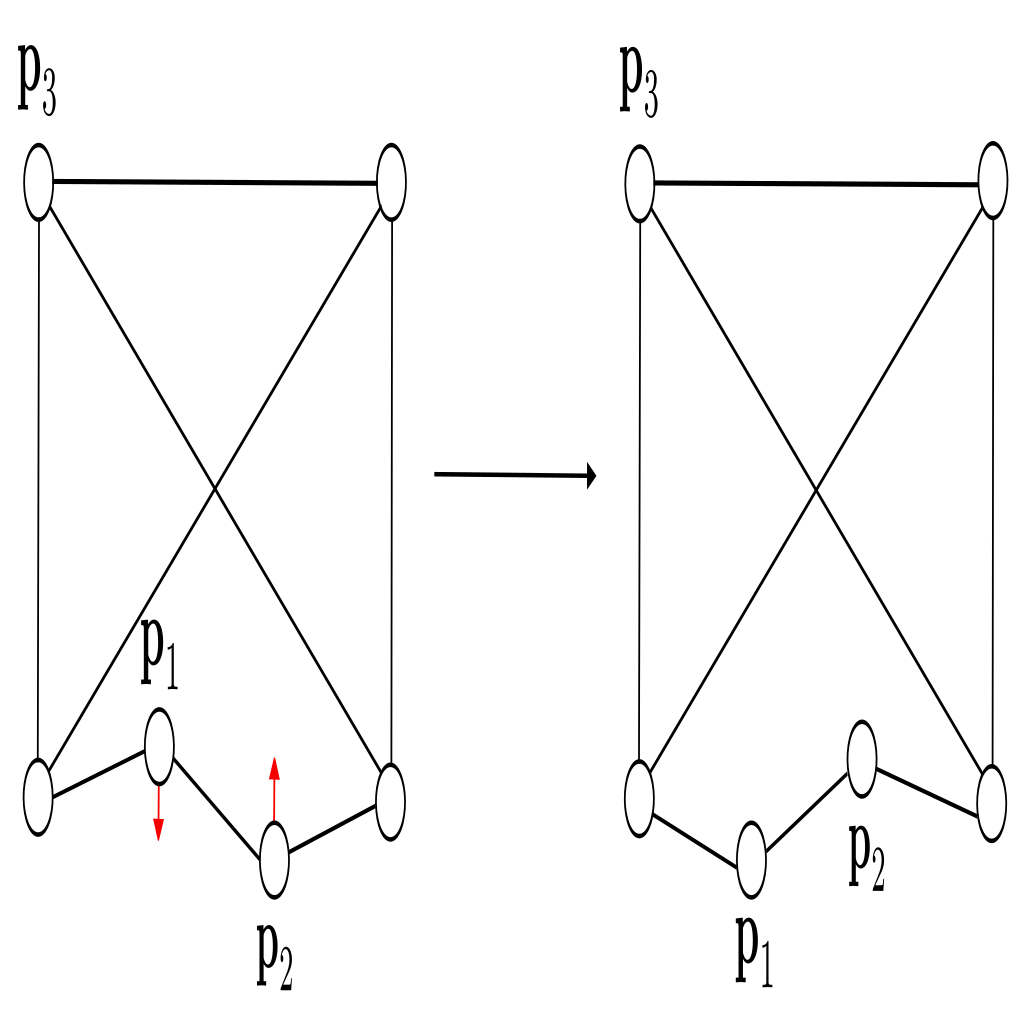
\includegraphics[width = 0.7\textwidth]{Chapter 2/10. not_inf_rigid_2.0.png}
    \caption{A framework that is not infinitesimally rigid}
    \label{eg: not inf rigid 2.0}
\end{figure}

\noindent
By applying instantaneous velocities to nodes $1$ and $2$ as shown in the framework on the left of Figure \ref{eg: not inf rigid 2.0}, we restructure the framework such that all the edge lengths are kept constant. This is shown in the framework on the right. However, the distance between nodes $1$ and $3$ have been altered. Therefore, this framework is not infinitesimally rigid.     

\begin{figure}[htbp]
    \centering
    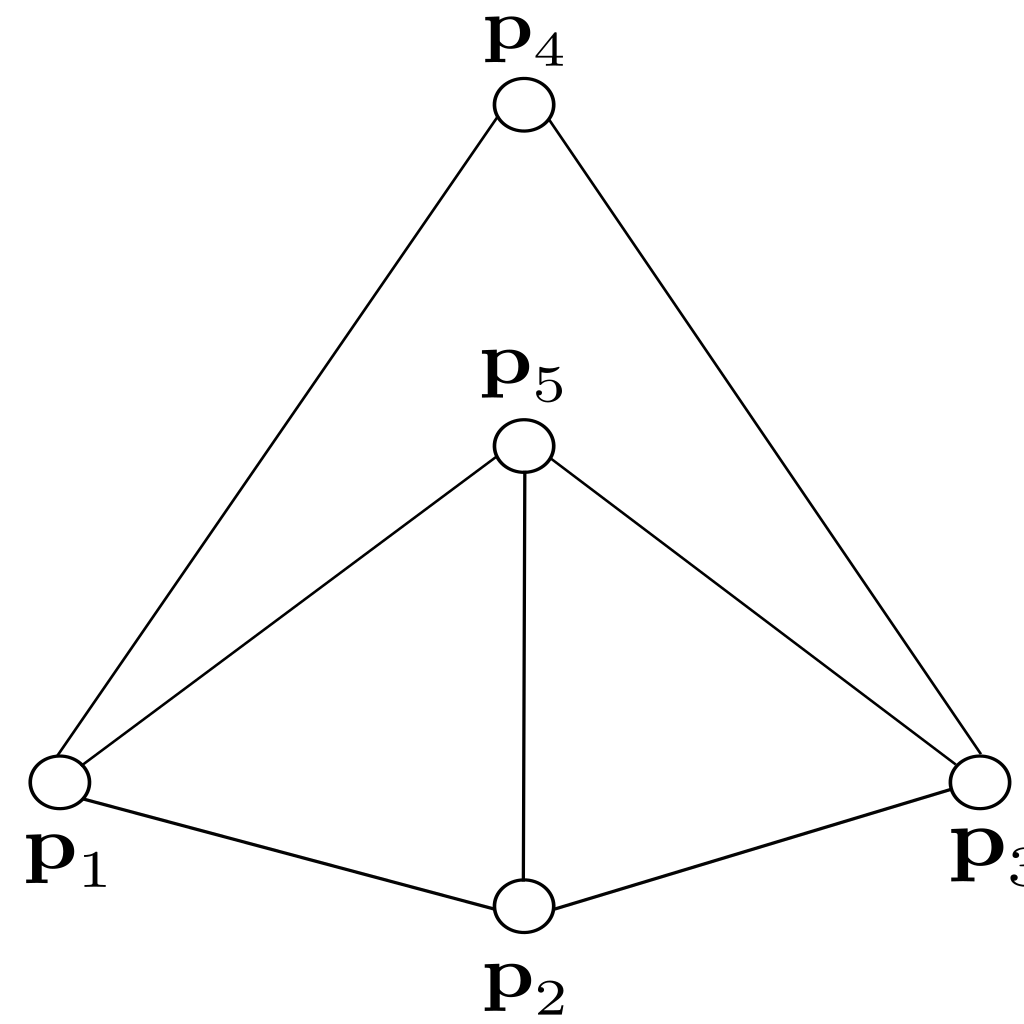
\includegraphics[width = 0.35\textwidth]{Chapter 2/11. inf_rigid.png}
    \caption{An infinitesimally rigid framework}
    \label{eg: inf rigid}
\end{figure}

\begin{flushleft}
Now consider the framework in Figure \ref{eg: inf rigid}. As we will soon see, triangular frameworks are infinitesimally rigid by a process known as a Henneberg construction of the first kind \cite{henneberg}. So this means that the framework can not be deformed by applying instantaneous velocities to nodes $1,2,3$  or $5$.     
\end{flushleft}

\begin{flushleft}
As the only way we can possible deform this framework is by applying some velocity to $4$, let us displace $4$ by an infinitesimal distance, say to the left without loss of generality. As our edges are of a fixed length, this will require edge $34$ to `pull' node $3$ upwards with the motion. As triangles $235$ and $125$ are known to be rigid, this causes the entire framework to rotate in an anti-clockwise fashion.
\end{flushleft}

\noindent
We already know that rotations are (infinitesimal) rigid motions, and so any displacement of the node $4$ results in an infinitesimal rigid motion. Therefore, we conclude that the framework in \hyperref[eg: inf rigid]{Figure 1.5} is infinitesimally rigid.
\end{example}

\subsection{Generic Rigidity}
We close this chapter on one last interesting way to classify rigidity. When studying configurations, we are interested in those that have nothing `special' about the way the points are arranged. Such configurations are known to be \textit{generic}.

\begin{flushleft}
To begin, we define a simpler result in order to get a feel for what we mean by not `special'.    
\end{flushleft}

\begin{definition}
Let $\mathbf{p} \in \mathbb{R}^d$ be a configuration. Then $\mathbf{p}$ is in \textit{general position} if any $d+1$ number of points do not lie in an $d-1$ dimensional affine space for $d>0$.
\end{definition}

\begin{flushleft}
Don't worry about what an affine space is as it is beyond the scope of this project! The definition essentially says that for a set of points to be in general position, we must \textbf{not} have:
\begin{itemize}
    \item Any two points that coincide at the same point when $d = 1$.
    \vspace{-3mm}
    \item Any three points that lie on the same line when $d = 2$.
    \vspace{-3mm}
    \item Any four points that lie on the same plane when $d = 3$.
\end{itemize}

And the pattern continues. This gives us a set of points that are spread out, making them more interesting to study.
\end{flushleft}

\begin{flushleft} % example of how 3 points satisfy a straight line equation. 
Genericity is a stronger condition than that of general position. The definition is as follows.
\end{flushleft}

\begin{definition}
A configuration $\mathbf{p}$ is \textit{generic} if the only polynomial with coefficients from $\mathbb{Q}$ that the coordinates of each point in $\mathbf{p}$ satisfies is the zero polynomial.
\end{definition}

\begin{flushleft}
A couple examples of point-sets that are not generic by this definition include four points on a circle and a pair of points on a line that has a rational slope \cite{textbook}. Our definitions of infinitesimal rigidity only apply to configurations that are generic, as we will see when considering the framework $(G,\mathbf{p})$ in Figure \ref{fig: non-generic}.
\end{flushleft}

\begin{figure}[htbp]
    \centering
    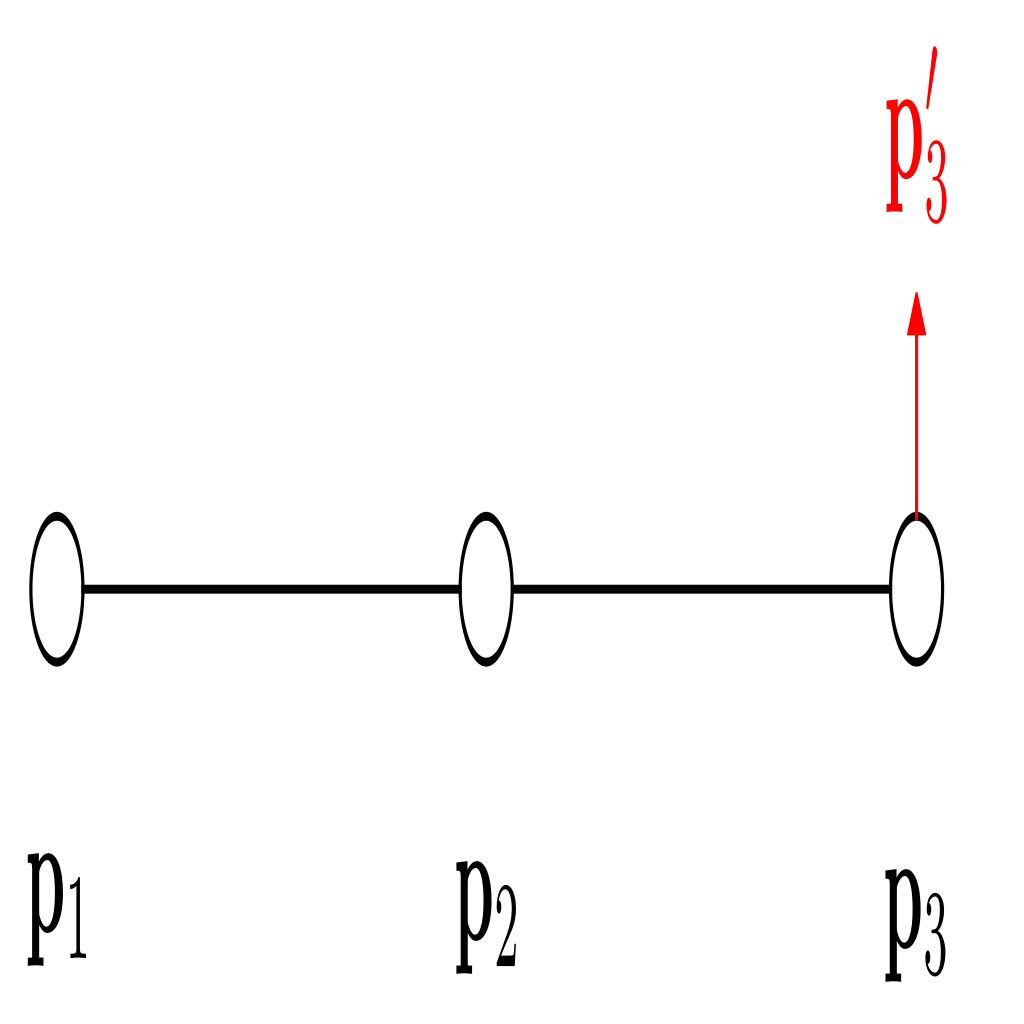
\includegraphics[width = 0.4\textwidth]{Chapter 2/16. generically_rigid.png}
    \caption{A non-generic framework in $\mathbb{R}^2$ with a non-zero instantaneous velocity applied to $\mathbf{p}_3$.}
    \label{fig: non-generic}
\end{figure}

\vspace{-2mm}
\begin{flushleft}
Here, the three nodes lie on a straight line and so they are not in general position which means they are not generic. Suppose we apply instantaneous velocities $\mathbf{p}'_1$, $\mathbf{p}'_2$ of magnitude 0 to the nodes $\mathbf{p}_1$ and $\mathbf{p}_2$, and apply the instantaneous velocity $\mathbf{p}'_3 = (0,k)$ to the node $\mathbf{p}_3$.
\end{flushleft}

\begin{flushleft}
By observation, we can tell that this framework is not infinitesimally rigid. By fixing nodes $\mathbf{p}_1$ and $\mathbf{p}_2$ in space, we may rotate the edge $\mathbf{p}_2\mathbf{p}_3$ about $\mathbf{p}_2$, thereby changing the distance between the nodes $\mathbf{p}_1$ and $\mathbf{p}_3$. 
\end{flushleft}

\begin{flushleft}
By computing the scalar products stated in Definition \ref{def: inf motion}, we see that 
\end{flushleft}
\vspace{-0.5mm}
\[
(\mathbf{p}_1 - \mathbf{p_2}) \cdot (\mathbf{p}'_1 - \mathbf{p}'_2) = (\mathbf{p}_2 - \mathbf{p_3}) \cdot (\mathbf{p}'_2 - \mathbf{p}'_3) = 0
\]

\begin{flushleft}
for both edges $\mathbf{p}_1\mathbf{p}_2$ and $\mathbf{p}_2\mathbf{p}_3$. However, 
\end{flushleft}
\vspace{-0.5mm}
\[
(\mathbf{p}_1 - \mathbf{p_3}) \cdot (\mathbf{p}'_1 - \mathbf{p}'_3) = 0
\]

\begin{flushleft}
as $\mathbf{p}'_3$ is perpendicular to the line passing through $\mathbf{p}_1\mathbf{p}_3$, stating that this framework is infinitesimally rigid. 
\end{flushleft}

\begin{flushleft}
For this reason, the frameworks we concern ourselves with will be defined on generic coordinates. Finally, we conclude with what it means to be generically rigid.    
\end{flushleft}

\begin{theorem}
\label{def: generic rigid}
If $(G,\mathbf{p})$ is an infinitesimally rigid framework in $\mathbb{R}^d$, then $(G,\mathbf{q})$ is infinitesimally rigid for any generic configuration $\mathbf{q}$.
\end{theorem}

\begin{flushleft}
This is an extremely powerful result. If we can find a configuration $\mathbf{p} \in \mathbb{R}^d$, generic or not, such that $(G,\mathbf{p})$ is infinitesimally rigid, then Definition \ref{def: generic rigid} implies that for \textit{any} generic configuration $\mathbf{q}$, we can find a framework with the same underlying graph $G$, such that it is also infinitesimally rigid.
\end{flushleft}

\begin{definition}
A configuration $(G,\mathbf{p})$ is \textit{generically rigid} in $\mathbb{R}^d$ if it is infinitesimally rigid for any one configuration $\mathbf{p}$.
\end{definition}

\begin{flushleft}
With that, we conclude this introductory exploration into the definitions of rigidity. These concepts form the basis of everything that is to come in later chapters. 
\end{flushleft}

\begin{flushleft}
Our current objective is unravelling the multitude of theorems that surround the study of rigid graphs. Through collecting as many tools revolving around rigidity and circle packings as possible and by invoking these ideas, we will be ever closer to understanding the structure of the special case of packings this project focuses on.
\end{flushleft}

\clearpage

%----------------------------------------------------------------------

\chapter{Exploring Rigidity \& Circle Packings}  % Is it Rigid?

\begin{flushleft}
So far, we have seen the various definitions of rigidity that we can use to identify whether a given framework is rigid. However, we have no methods or techniques we can use in order to \textit{test} for the rigidity of a framework. We also don't know how the various definitions of rigidity get along with each other. If a framework is rigid, does it mean its infinitesimally rigid? Can we test for infinitesimal rigidity in some way? % find a third question
\end{flushleft}

\begin{flushleft}
In addition to these questions, we will also introduce circle packings, and discuss how they come about. As rigidity can't be tested merely by observation, testing the rigidity of a circle packing arises from using a few techniques seen earlier. For the remainder of this project, we will be working exclusively in $\mathbb{R}^2$ unless specified otherwise.
\end{flushleft}

\section{Degrees of Freedom}

\noindent
This section has been adapted from Graver's book \cite{counting_frameworks}.

\begin{flushleft}
To understand what it means for a framework to have $x$ number of \textit{degrees of freedom}, let us first go through some simple examples to gain an understanding of what a degree of freedom is.

\begin{itemize}
    \item Consider a point in $\mathbb{R}^2$. It can move right or left along the $x$-axis, or up and down along the $y$-axis. As it can travel along either axis, we say that this point has two \textit{degrees of freedom}. 
    \item Now, if we consider a line segment $l$ in the plane with two endpoints, we know that each endpoint has two degrees of freedom, giving us four degrees of freedom, but the line between them prevents the endpoints from moving independently of each other. So, $l$ can move either along the $x$ or $y$-axes, giving us two degrees of freedom. However, it can also rotate about some point in $\mathbb{R}^2$. Therefore, such a segment has three degrees of freedom.
    \item If we were to consider a point in $\mathbb{R}^3$, then as the point can travel along the $x$, $y$ or $z$-axes, it has three degrees of freedom. 
\end{itemize}
\end{flushleft}

\begin{flushleft}
At this point, we should be able to see what a degree of freedom means. It is essentially a count of how many ways we can move a structure (or frameworks in our case) around in space. Additionally, we can note that adding an edge between two points reduces the total degrees of freedom in the system from four to three due to the constraint that the points can't move independently of each other. 
\end{flushleft}
\vspace{-3 mm}
\begin{figure}[htbp]
    \centering
    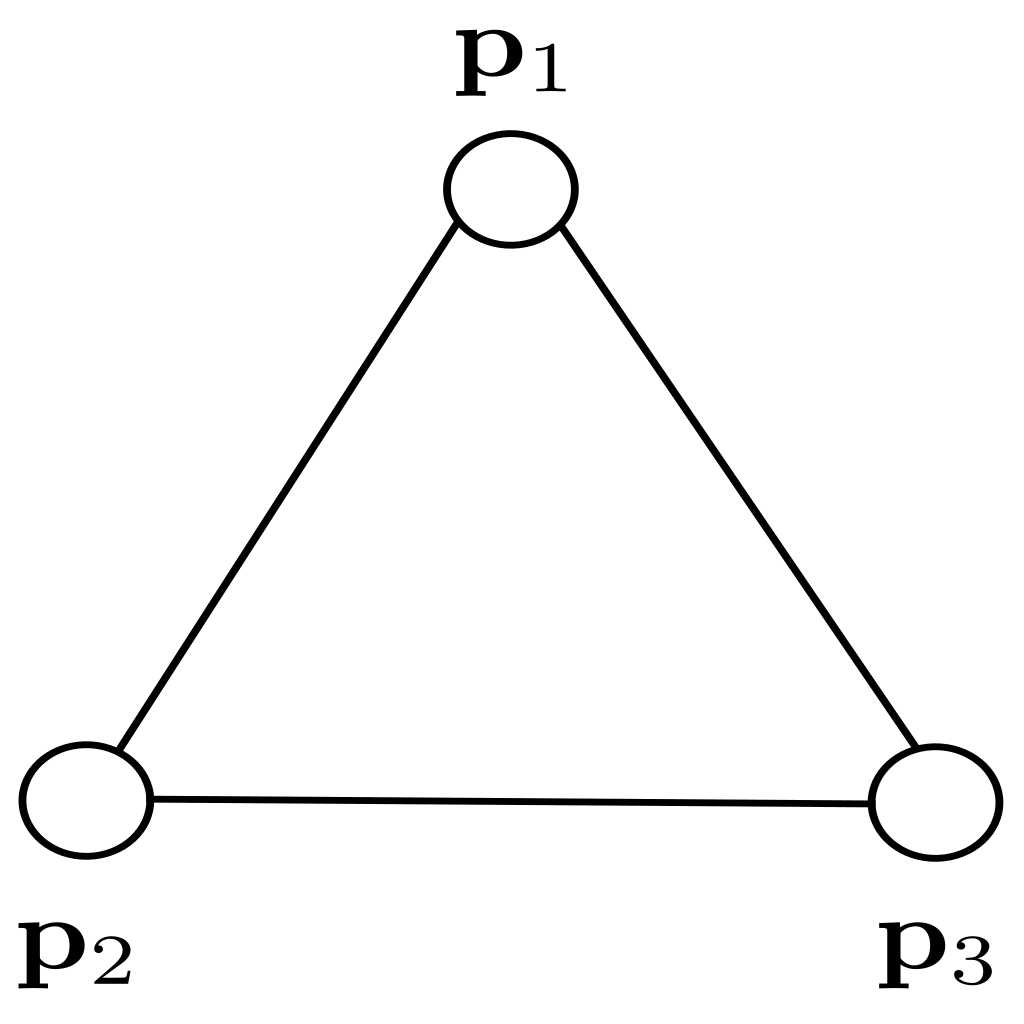
\includegraphics[width = 0.25\textwidth]{Chapter 3/5. degree_of_freedom.png}
    \caption{A framework on three nodes and three edges}
    \label{fig: degree_of_freedom}
\end{figure}

\begin{example}
In order to find how many degrees of freedom the framework in Figure \ref{fig: degree_of_freedom} has, we start with just three nodes, and then build up to the framework given:
\begin{itemize}
    \item With only three nodes in the plane, and each node having two degrees of freedom, the total degrees of freedom the system has is $3 \times 2 = 6$.
    \item If we add an edge between $\mathbf{p}_1$ and $\mathbf{p}_2$ now, we lose a degree of freedom, giving us $3$ degrees of freedom for the segment and $2$ for the segment, totalling $5$ degrees of freedom in the system.
    \item Adding the edge between $\mathbf{p}_1$ and $\mathbf{p}_3$, we further reduce the number of ways the framework can move: $3$ degrees of freedom for the first segment and $1$ degree of freedom for rotation of the second segment about their common endpoint. At this stage, the structure has $4$ degrees of freedom.
    \item Adding the last edge between $\mathbf{p}_2$ and $\mathbf{p}_3$ gives us the framework in question. We reduce the degrees of freedom by one yet again, giving us $3$ degrees of freedom in total now.
\end{itemize}
\end{example}

\begin{flushleft}
Using Definition \ref{def: rigid}, we know that for any (infinitesimally) rigid body in the plane, we must only be allowed to translate it along the two axes, as well as only rotate it about some point.
\end{flushleft}

\begin{theorem}
\label{thm: degrees of rigid body}
In $\mathbb{R}^2$, any rigid body must have $3$ degrees of freedom. 
\end{theorem}

\section{The Rigidity Matrix}

\begin{flushleft}
When given a framework, it can be quite difficult to tell whether it is rigid or not. This is where the \textit{rigidity matrix} comes in. By finding a way to encode a framework into a matrix, we can then use tools from linear algebra to study and draw conclusions about the framework itself!
\end{flushleft}

\begin{definition}
\label{def: rigidity matrix}
The \textit{rigidity matrix} $\mathbf{R}(G,\mathbf{p})$ of a $d$-dimensional framework $(G,\mathbf{p})$ is a matrix that contains the system of equations described in Definition \ref{def: inf motion}. It is a $|E(G)| \times d|V(G)|$ matrix, where the rows are indexed by the edges of $G$, and sets of $d$ consecutive columns correspond to a single node of $(G,\mathbf{p})$. 

\noindent
If there is an edge between nodes $\mathbf{p}_i$ and $\mathbf{p}_j$ when $d=2$, then the non-zero entries in the corresponding row of the matrix lie in columns corresponding to coordinates of each node. That is;
\begin{itemize}
    \item Columns $2i-1$ and $2i$ corresponding to the coordinates of node $p_i$.
    \vspace{-3mm}
    \item Columns $2j-1$ and $2j$ corresponding to the coordinates of node $p_j$.
    \vspace{-3mm}
    \item $0$ everywhere else.
\end{itemize}
\end{definition}

\begin{figure}[htbp]
    \centering
    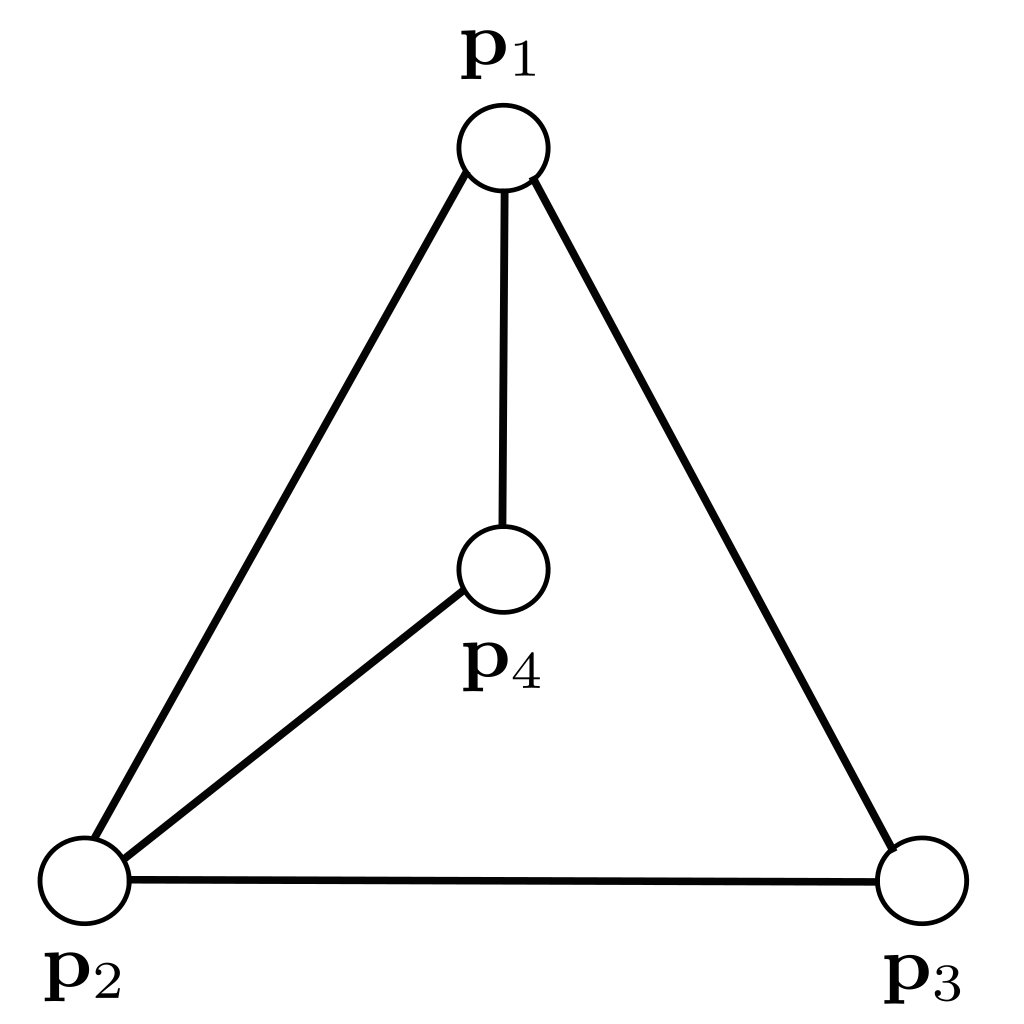
\includegraphics[width = 0.25\textwidth]{Chapter 3/4. rigidity_matrix.png}
    \caption{A framework on four nodes and five edges.}
    \label{fig: rigidity_matrix}
\end{figure}
\vspace{-3 mm}
\begin{flushleft}
For example, consider the framework $(G,\mathbf{p})$ in Figure \ref{fig: rigidity_matrix}. As we are working in $\mathbb{R}^2$, we know that $\mathbf{p}_i = (x_{i}, y_{i})$, for each $i = 1,2,3,4$. Therefore, we can construct $\mathbf{R}(G,\mathbf{p})$ as
\end{flushleft}
\vspace{-6 mm}
\begin{center}
\begin{tabular}{ c c } 
 & \underline{Edges} \\
\multirow{5}{15 cm}{$
    \mathbf{R}(G,\mathbf{p}) = 
    \begin{bmatrix}
    x_1 - x_2 & y_1 - y_2 & x_2 - x_1 & y_2 - y_1 & 0 & 0 & 0 & 0 \\ %p1p2
    x_1 - x_3 & y_1 - y_3 & 0 & 0 & x_3 - x_1 & y_3 - y_1 & 0 & 0 \\ %p1p3
    x_1 - x_4 & y_1 - y_4 & 0 & 0 & 0 & 0 & x_4 - x_1 & y_4 - y_1 \\ %p1p4
    0 & 0 & x_2 - x_3 & y_2 - y_3 & x_3 - x_2 & y_3 - y_2 & 0 & 0 \\ %p2p3
    0 & 0 & x_2 - x_4 & y_2 - y_4 & 0 & 0 & x_4 - x_2 & y_4 - y_2 \\ %p2p4
    \end{bmatrix}$} & $\mathbf{p}_1\mathbf{p}_2$ \\
    & $\mathbf{p}_1\mathbf{p}_3$ \\
    & $\mathbf{p}_1\mathbf{p}_4$ \\
    & $\mathbf{p}_2\mathbf{p}_3$ \\
    & $\mathbf{p}_2\mathbf{p}_4$ \\    
\end{tabular}
\end{center}
\vspace{0.5 mm}
\begin{flushleft}
The rows of $\mathbf{R}(G,\mathbf{p})$ correspond to the edges in $(G,\mathbf{p})$, and each consecutive set of two columns correspond to the $x$ and $y$ coordinates of each node in $\mathbf{p}$, leading to the creation of $2 \times 4 = 8$ columns and $5$ rows in $\mathbf{R}(G,\mathbf{p})$.
\end{flushleft}

\begin{example}
\label{eg: rigidity matrix}
Let the framework $(G,\mathbf{p})$ be the one in Figure \ref{fig: rigidity_matrix}. If we give the nodes of $(G,\mathbf{p})$ positions in $\mathbb{R}^2$, we can compute its numeric rigidity matrix $\mathbf{R}(G,\mathbf{p})$. 

\noindent
Suppose that $\mathbf{p}_1 = (1,2)$, $\mathbf{p}_2 = (0,0)$, $\mathbf{p}_3 = (2,0)$, $\mathbf{p}_4 = (1,1)$. Then, the rigidity matrix $\mathbf{R}(G,\mathbf{p})$ is

\[
\mathbf{R}(G,\mathbf{p}) = 
\begin{bmatrix}
1 & 2 & -1 & -2 & 0 & 0 & 0 & 0 \\
-1 & 2 & 0 & 0 & 1 & -2 & 0 & 0 \\
0 & 1 & 0 & 0 & 0 & 0 & 0 & -1 \\
0 & 0 & -2 & 0 & 2 & 0 & 0 & 0 \\
0 & 0 & -1 & -1 & 0 & 0 & 1 & 1 \\
\end{bmatrix}
\]
\end{example}

\begin{flushleft}
Now that we have the rigidity matrix, we can use it to determine whether a given d-dimensional framework is infinitesimally rigid or not. Recalling Definition \ref{def: inf motion}, we can see that the space of infinitesimal motions of a framework $(G,\mathbf{p})$ is equal to the kernel of $R(G,\mathbf{p})$, denoted Ker($\mathbf{R}$).

By using a result from Linear Algebra known as the \textbf{Rank-Nullity Theorem}, we see that
\vspace{-1 mm}
\[
\text{rank}(\mathbf{R}) + \text{dim}(\text{Ker}(\mathbf{R})) = d|V|
\]

\end{flushleft}

\begin{flushleft}
As the space of infinitesimal rigid motions govern the number of ways a framework can move in space, we can deduce that a useful result.
\end{flushleft}

\begin{lemma}
Let $(G,\mathbf{p})$ be a framework, and $\mathbf{R}(G,\mathbf{p})$ be its rigidity matrix. Then $(G,\mathbf{p})$ has $dim(\text{Ker}(\mathbf{R}))$ degrees of freedom. 
\end{lemma}

\begin{flushleft}
As we're concerned with frameworks in $\mathbb{R}^2$, using Theorem \ref{thm: degrees of rigid body}, we know that rigid frameworks must have $3$ degrees of freedom. From Definition \ref{def: inf rigid}, we deduce the following theorem.
\end{flushleft}

\begin{theorem}
\label{thm: rank-rigid}
Let $(G,\mathbf{p})$ be a framework and $\mathbf{R}(G,\mathbf{p})$ be its rigidity matrix. Then, $(G,\mathbf{p})$ is infinitesimally rigid in $\mathbb{R}^2$ if and only if 
\[
\text{rank}(\mathbf{R}) = 2|V| - 3
\]
\end{theorem}

\begin{flushleft}
We have now successfully used techniques from linear algebra in order to test for infinitesimal rigidity of a framework! This result was proved by Asimow and Roth in their paper \cite{asimow}, and is going to be a pertinent to this project. Being able to analyze frameworks using matrices enables us to computationally investigate properties of the matrix, allowing for a speedy analysis of a given framework.
\end{flushleft}

\section{Constructing Rigid Structures}
Through an algorithmic process of adding nodes and deleting edges, we can create frameworks such that they are rigid in nature. This is done using the Henneberg construction \cite{henneberg}. However, in order to end up with a rigid framework, we must start with a graph known as a \textit{Laman Graph}.

\begin{definition}
\label{def: laman graph}
Let $G = (V,E)$ be a connected graph, and let $H$ be a subgraph of $G$. Then $G$ is known as a \textit{Laman graph} if
\begin{itemize}
    \item The edge set of $G$ has size $|E(G)| = 2|V(G)| - 3$.
    \item For any subgraph $H$ defined on $k \leq |V(G)|$ vertices, $|E(H)| \leq 2k-3$.
\end{itemize}
as defined in \cite{laman_graph}.
\end{definition}

\begin{flushleft}
Such graphs are named after Gerard Laman, who studied the rigidity of graphs in the 1970s. 

Now, a question we can ask at this stage is if we can find graphs that are rigid on the smallest number of edges possible. That is, are there rigid graphs such that if we take away an edge, it causes the structure to lose its rigidity? Such graphs are known to be \textit{minimally rigid}.
\end{flushleft}

\begin{flushleft}
As this project revolves around minimally rigid graphs, it is important to learn what graphs are minimally rigid, and if there's a way to identify which graphs are classed as minimally rigid. 
\end{flushleft}

\begin{theorem}
\label{thm: laman = minimally rigid}
A graph $G$ is minimally rigid in $\mathbb{R}^2$ if and only if $G$ is a Laman graph \cite{minimally_rigid}.
\end{theorem}

\begin{flushleft}
Therefore, a graph $G$ is minimally rigid if and only if $G$ has $2n-3$ edges, where $n = |V(G)|$. This is known as the Geiringer–Laman theorem, as it was first proved by Hilda Pollaczek-Geiringer in 1927 \cite{laman_theorem}, and then independently by Laman in 1970 \cite{minimally_rigid}.
\end{flushleft}

\begin{flushleft}
Given such a characterization, we can now talk about ways to construct minimally rigid graphs, of which there are two we focus on. They are known as the \textit{Henneberg constructions} \cite{henneberg}.
\end{flushleft}

\begin{definition}
\label{def: henneberg}
The \textit{Henneberg construction} in $\mathbb{R}^2$ involves two processes in order to generate minimally rigid graphs.
\begin{itemize}
    \item Type I: To an existing Laman graph $G$, insert a new vertex $u$ and attach it to $G$ by adding two edges between $u$ and two distinct vertices in $G$.
    \item Type II: To an existing Laman graph $G$, delete an edge between two vertices $v_1,v_2 \in V(G)$, insert a new vertex $u$, and attach it to $G$ by adding edges between $u$ and $v_1$, $v_2$ and one other vertex in $G$. 
\end{itemize}
\noindent
The resulting graph will be have $2|V(G)|-3$ edges, and is therefore minimally rigid by Theorem \ref{thm: laman = minimally rigid}.
\end{definition}

\begin{example}
A sequence of constructions using Henneberg Type I and Type II are shown.

\begin{figure}[htbp]
    \centering
    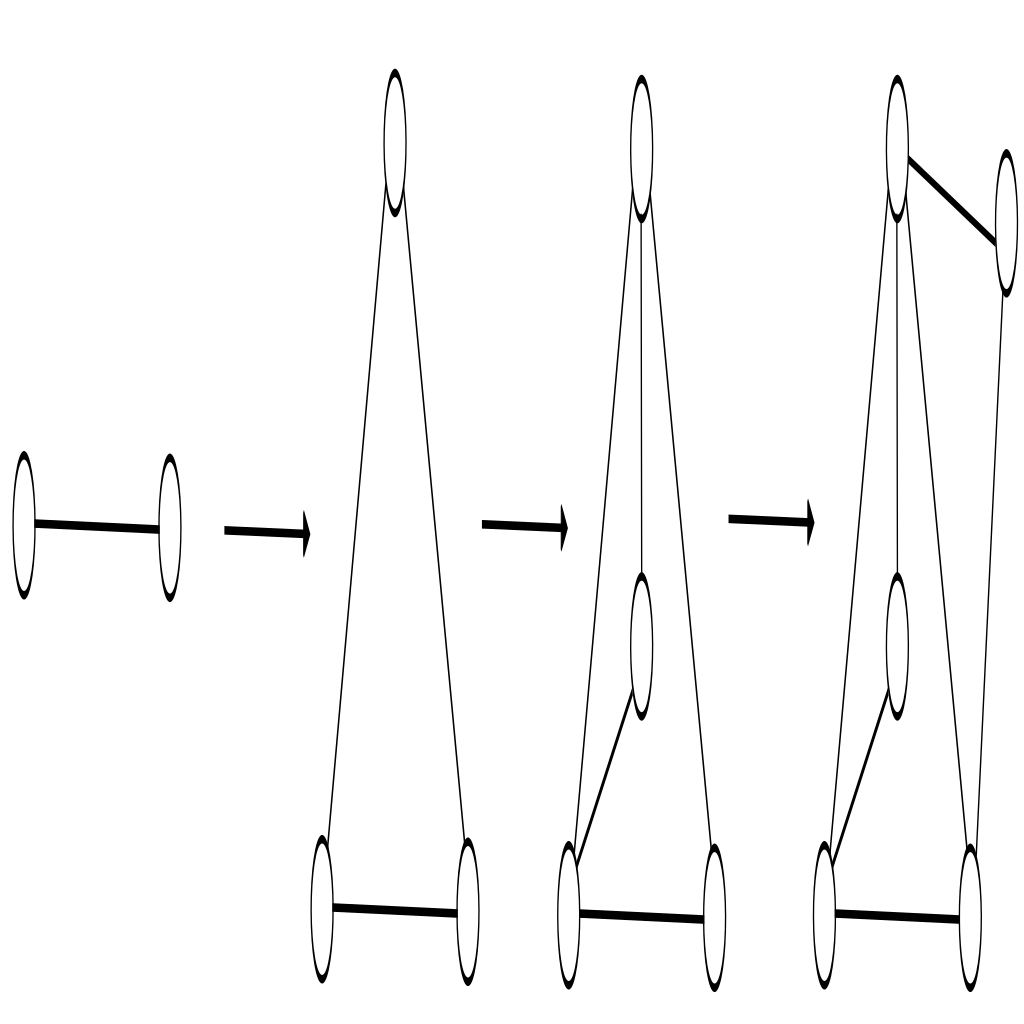
\includegraphics[width = 0.9\textwidth]{Chapter 3/2. henneberg_1.png}
    \caption{A series of constructions created solely using Henneberg Type I}
    \label{fig: henneberg 1}
\end{figure}

\begin{figure}[htbp]
    \centering
    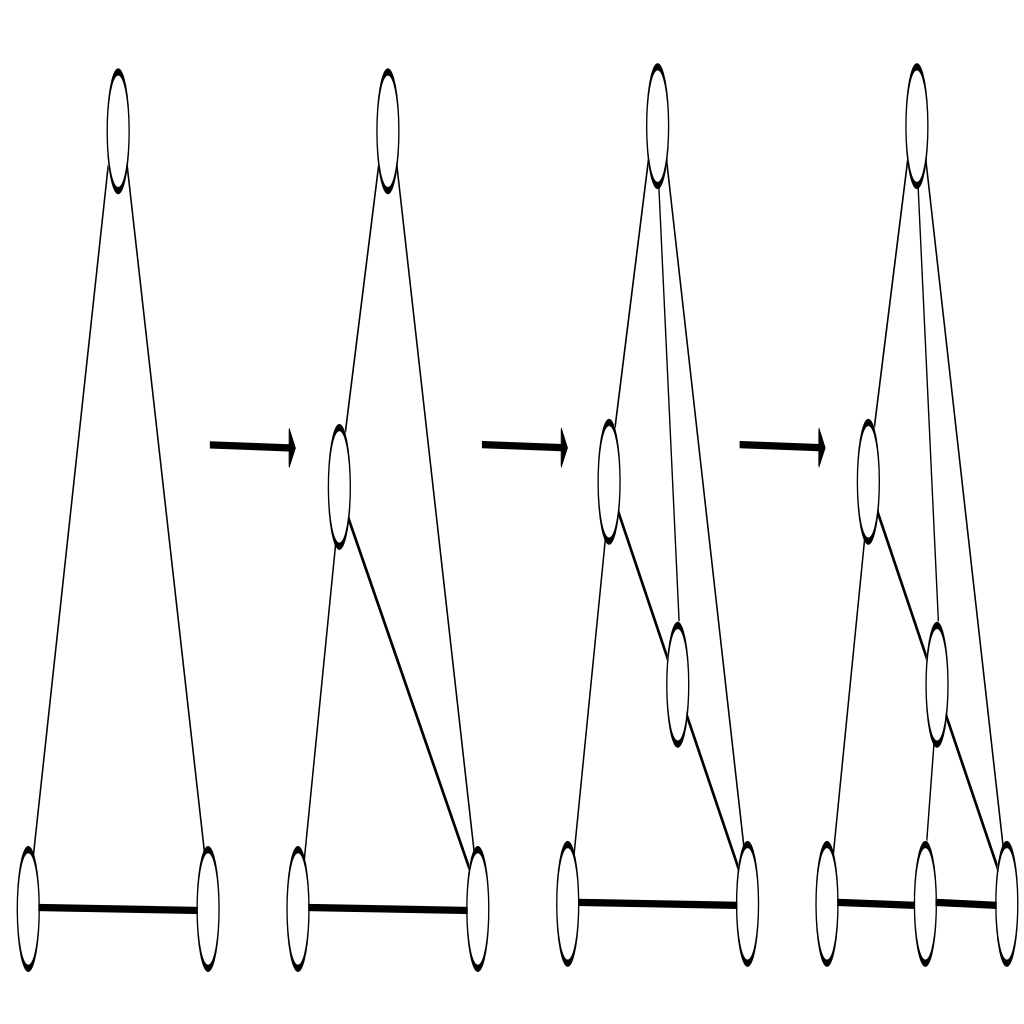
\includegraphics[width = 0.9\textwidth]{Chapter 3/3. henneberg_2.png}
    \caption{A series of constructions created solely using Henneberg Type II}
    \label{fig: henneberg 2}
\end{figure}
\noindent
By checking directly, we can verify that the graphs at each stage are indeed Laman graphs.
\end{example}

\begin{flushleft}
With the use of the rigidity matrix, or simply by observation, we can see that frameworks at each stage of the Henneberg constructions are infinitesimally rigid. 
\end{flushleft}

\begin{corollary}
\label{cor: laman => inf rigid}
Let $(G,\mathbf{p})$ be a minimally rigid framework, where $G$ is a Laman graph. Then $(G,\mathbf{p})$ is infinitesimally rigid.
\end{corollary}

\section{Rigidity vs Infinitesimal Rigidity} 

\begin{flushleft}
At this stage, we have a good understanding of what rigidity and infinitesimal rigidity are. We have seen ways to check whether a framework is infinitesimally rigid, and learned of a method to construct minimally rigid graphs. In this section, the aim is to learn how one relates with the other. 
\end{flushleft}

\begin{figure}[htbp]
    \centering
    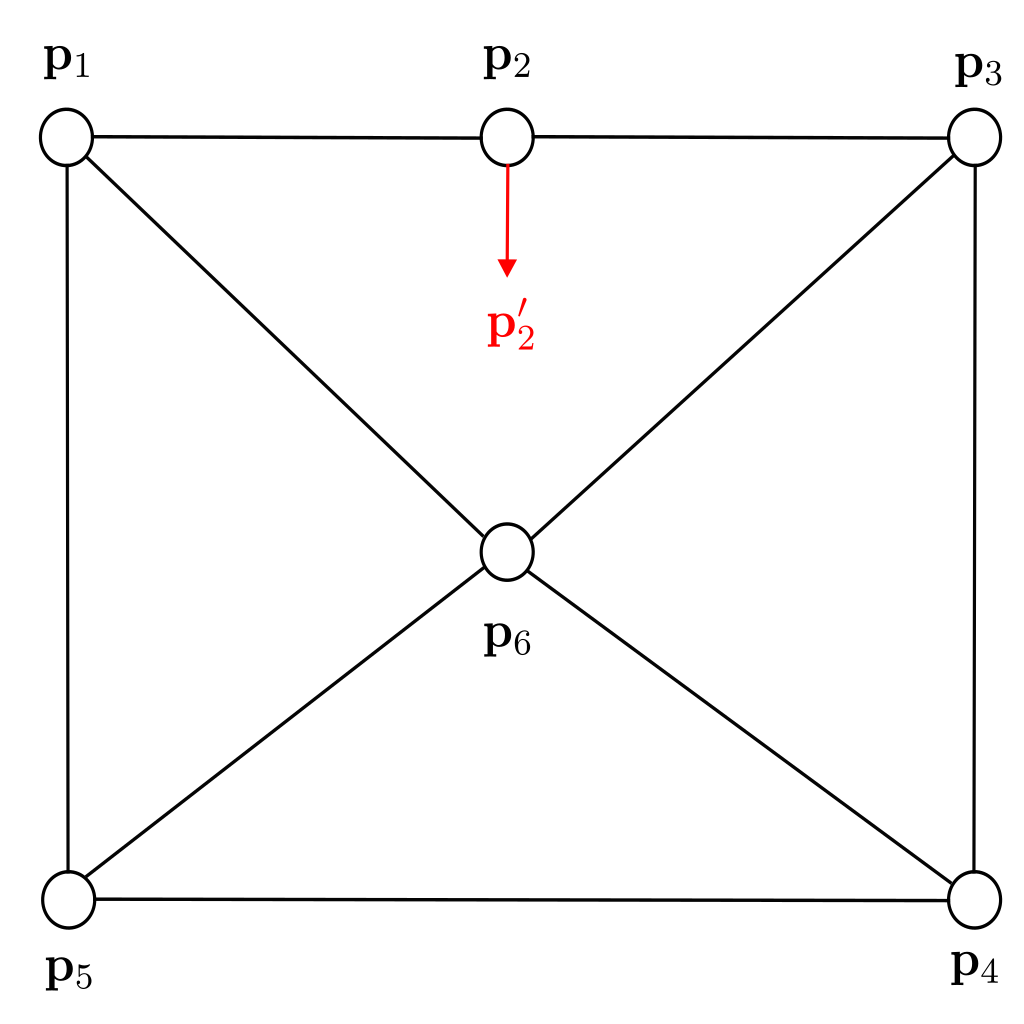
\includegraphics[width = 0.45\textwidth]{Chapter 3/6. rigid but not inf rigid.png}
    \caption{A rigid framework with an instantaneous velocity applied to $\mathbf{p}_5$ shown in red.}
    \label{fig: rigid but not inf rigid}
\end{figure}
\vspace{-4 mm}
\begin{flushleft}
To motivate this, let us consider the framework $(G,\mathbf{p})$ in Figure \ref{fig: rigid but not inf rigid}. As this framework is formed by joining two triangles together, we know it must be rigid as triangles are themselves rigid. The question is whether it is infinitesimally rigid. 
\end{flushleft}

\begin{flushleft}
Suppose we apply infinitesimal velocities of magnitude $0$ to nodes $\mathbf{p}_1$, $\mathbf{p}_2$, $\mathbf{p}_3$, $\mathbf{p}_4$, and we apply the infinitesimal velocity $\mathbf{p}'_5 \neq 0$ to node $\mathbf{p}_5$. We first verify whether these instantaneous velocities make an infinitesimal motion by checking $(\mathbf{p}_i - \mathbf{p}_j) \cdot (\mathbf{p}'_i - \mathbf{p}'_j) = 0$ for all $ij \in E(G)$. 

As each velocity vector is $0$ except for $\mathbf{p}'_5$, it follows that this is true for all the edges in $(G,\mathbf{p})$.
\end{flushleft}

\begin{flushleft}
Now, consider $(\mathbf{p}_5 - \mathbf{p}_2) \cdot (\mathbf{p}'_5 - \mathbf{p}'_2)$.The vector $(\mathbf{p}_5 - \mathbf{p}_2)$ is simply the line through the two nodes, which is non-zero, and $(\mathbf{p}'_5 - \mathbf{p}'_2) = \mathbf{p}'_5$ as $\mathbf{p}'_5$ is non-zero by assumption. As the vectors $(\mathbf{p}_5 - \mathbf{p}_2)$ and $\mathbf{p}'_5$ are not perpendicular to each other, it follows that,

\[
(\mathbf{p}_5 - \mathbf{p}_2) \cdot (\mathbf{p}'_5 - \mathbf{p}'_2) \neq 0
\]
\end{flushleft}

\begin{flushleft}
Therefore, this framework is not infinitesimally rigid. 
\end{flushleft}

\begin{flushleft}
This shows us that even though a framework might be rigid, it may not be infinitesimally rigid. Applying instantaneous velocities at a carefully selected node can very well deform a rigid structure. The converse however is true.
\end{flushleft}

\begin{theorem}
Let $(G,\mathbf{p})$ be a infinitesimally rigid framework. Then $(G,\mathbf{p})$ is rigid.
\end{theorem}

\begin{flushleft}
The proof of this theorem relies on a lot of heavy mathematics which is beyond the scope of this project, and it can be found in Asimow and Roth's paper \cite{asimow}. Therefore, infinitesimal rigidity is a stronger property than rigidity. 
\end{flushleft}

% flesh this out a little bit more. I'm unhappy with the way it ends off

\section{Circle Packings}

\begin{flushleft}
 In this last section, we finally come to circle packings and how they are defined. Additionally, we also learn how we can identify ways in which we can use the methods described earlier in order to test the rigidity of a packing. 
\end{flushleft}

\begin{figure}[htbp]
    \centering
    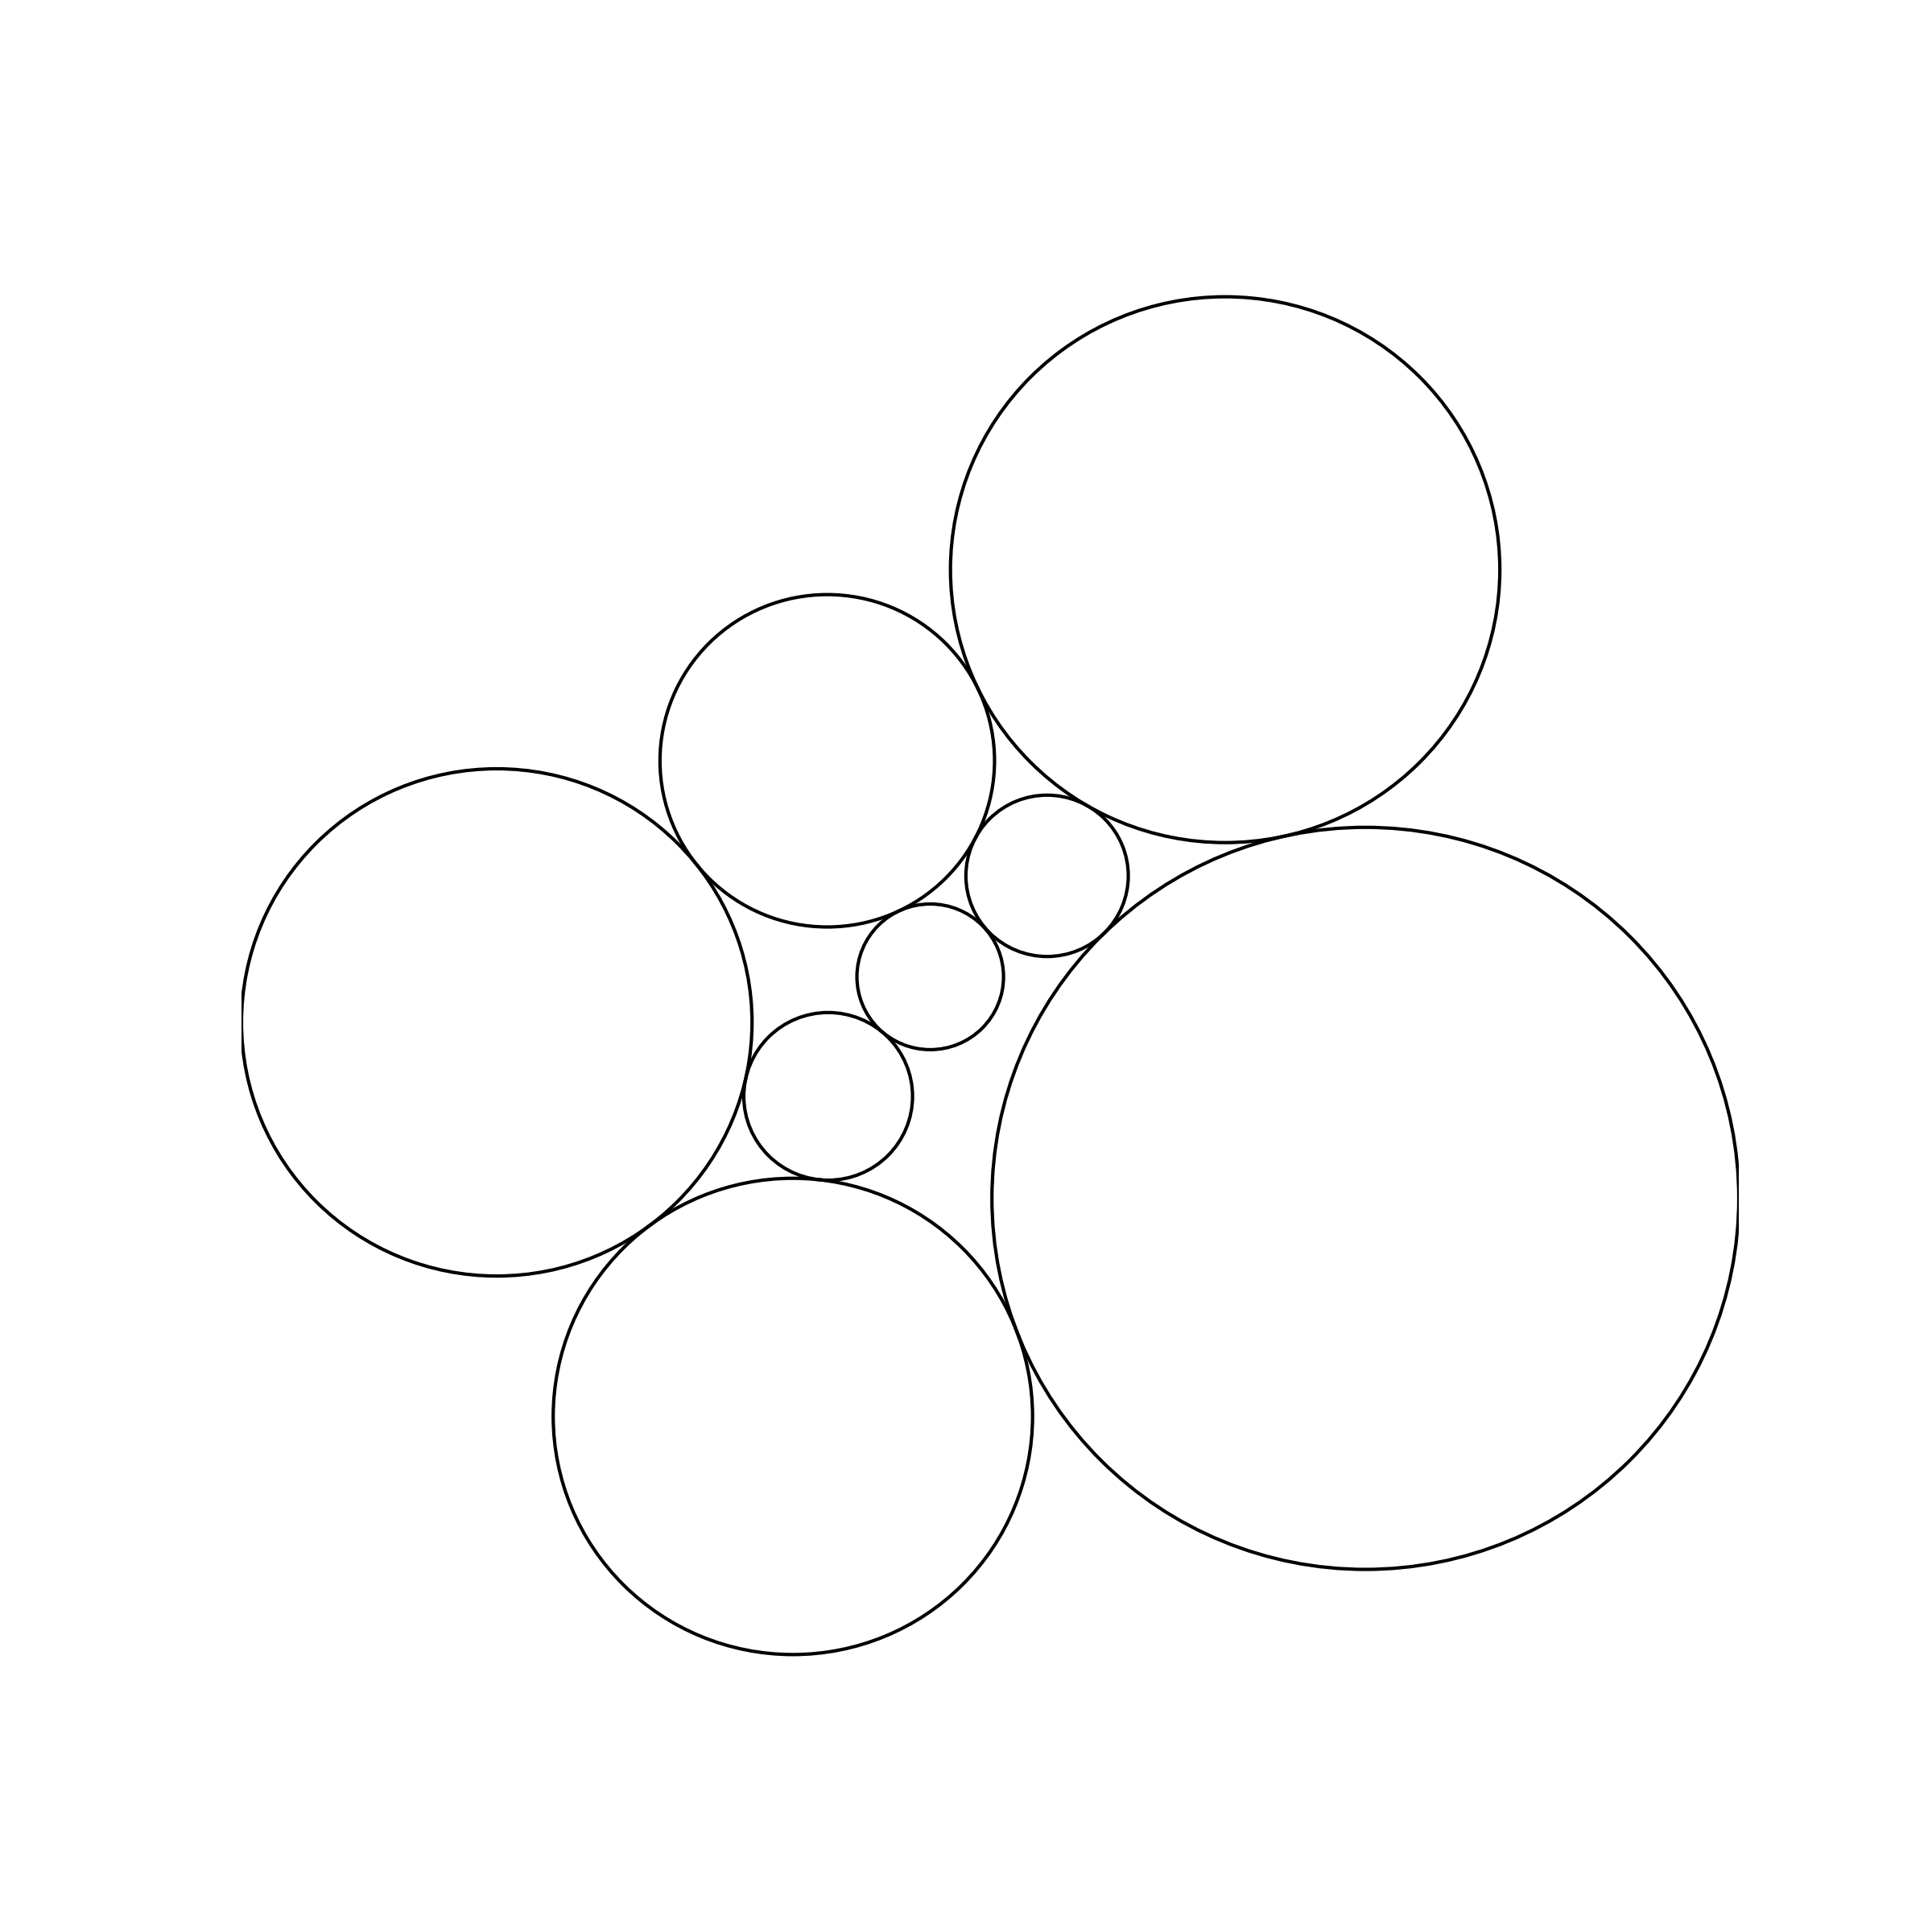
\includegraphics[width = 0.42\textwidth]{Chapter 3/7. Plain packing.png}
    \caption{A circle packing with 8 circles}
    \label{fig: circle packing example}
\end{figure}
\vspace{-4 mm}
\begin{flushleft}
Circle packings are configurations of circles satisfying preassigned patterns of tangency. They are designed such that each pair of circles may either touch tangentially, or not at all. Circles are not allowed to overlap or be contained in one another as well. An example of a circle packing is shown in Figure \ref{fig: circle packing example}. As we can see, not all of the circles have the same radius. This is necessary as the circles must be able to adjust their radii in order to fit tightly and satisfy any constraints imposed on them.
\end{flushleft}

\begin{definition}
\label{def: circle packing}
A \textit{circle packing} is a configuration of circles $P = (C_i)$, where $i \in \mathbb{Z}^+$, in the plane $\mathbb{R}^2$ such that any
two distinct circles in P have disjoint interiors. 

\noindent
That is, distinct circles in P may be tangent, but may not overlap.
\end{definition}

\begin{flushleft}
Given a circle packing, we must now find a way to analyze its properties. Thankfully, there is a natural way to encode the qualities of a packing $P$ into a graph $G(P)$, which we call the circle packing's \textit{contact graph}.
\end{flushleft}

\begin{definition}
\label{def: contact graph}
Let $P = (C_i)$ be a circle packing, where $i \in \mathbb{Z}^+$. Then, the \textit{contact graph} $G(P)$ of the packing $P$ is a graph where the vertex set is the set of circles in $P$, and an edge joins two vertices $u, v \in G(P)$ if an only if the circles corresponding to the vertices are tangential in $P$.
\end{definition}

\begin{flushleft}
In other words, an edge is added between two vertices in a contact graph if and only if the corresponding circles make \textit{contact}.
\end{flushleft}

\begin{flushleft}
We now have a way to encode a circle packing's properties into a graph! By observation, we can conclude that the contact graph $G(P)$ is always going to be a \hyperref[def: planar graphs]{planar} graph, as if edges were to cross over, this would imply that the corresponding circles in $P$ overlap each other. Studying a packing's contact graph allows us to invoke tools and methods we've developed so far in order to investigate the rigidity of the packing in question. 
\end{flushleft}

\begin{figure}[htbp]
    \centering
    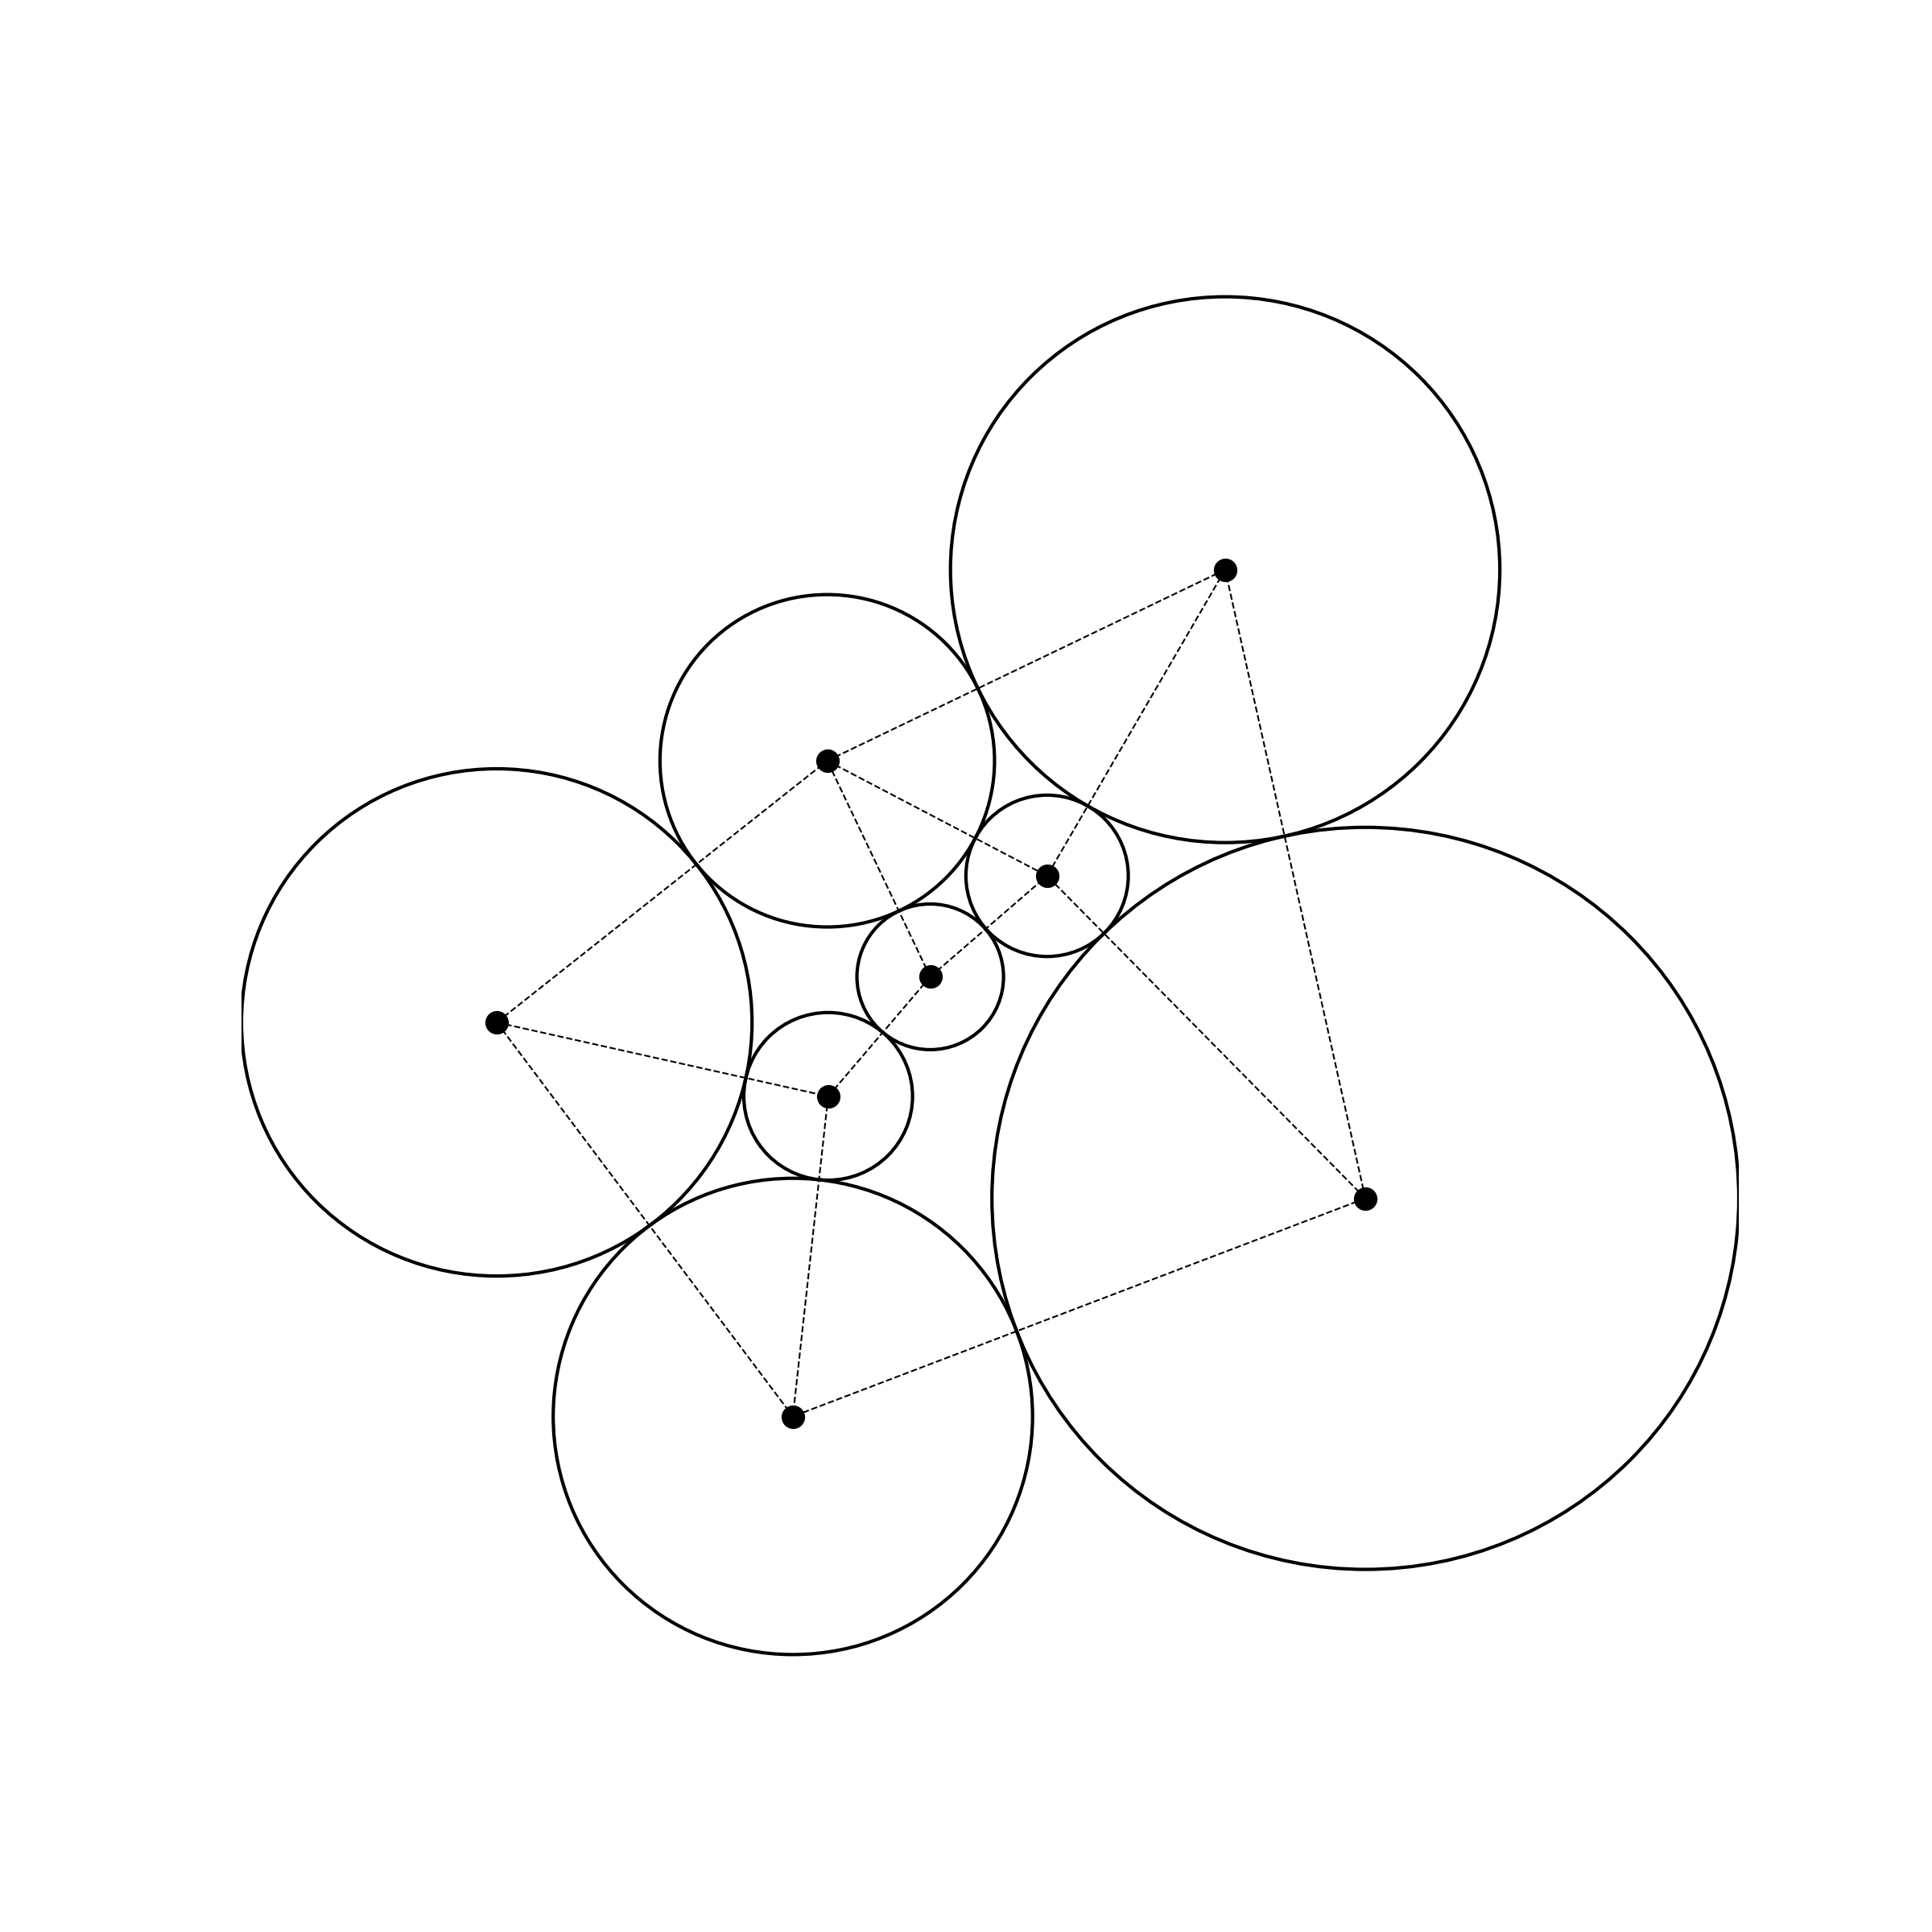
\includegraphics[width = 0.42\textwidth]{Chapter 3/8. Packing with contact.png}
    \caption{The circle packing from Figure \ref{fig: circle packing example} with its contact graph visualized}
    \label{fig: circle packing with contact}
\end{figure}
\vspace{-4 mm}
\begin{flushleft}
For a circle packing $P$, we now state that $P$ is infinitesimally rigid if its contact graph $G(P)$ is infinitesimally rigid \cite{sticky}. As rigidity does not imply infinitesimal rigidity, checking for infinitesimal rigidity is sufficient to verify the rigidity of the packing itself. 
\end{flushleft}

\begin{flushleft}
In Connelly, Gortler, and Theran's paper \cite{sticky}, the following theorem is proved.
\end{flushleft}

\begin{theorem}
\label{thm: louis thm}
Let $P = (C_i)$ be a circle packing, where $i = 1,2,\hdots, n$. Then if P has $2n-3$ contacts, it is rigid and infinitesimally rigid. If the number of contacts is fewer, then P is flexible and infinitesimally flexible.
\end{theorem}

\begin{flushleft}
This follows from investigating the contact graph $G(P)$ of a packing $P$. If the packing has $n$ circles, then there must be $n$ vertices in $G(P)$. Furthermore, if there are $2n-3$ contacts in $P$, then there must be $2n-3$ edges in $G(P)$.
\end{flushleft}

\begin{flushleft}
By Definition \ref{def: laman graph}, we know that $G(P)$ is a Laman graph, and by invoking Corollary \ref{cor: laman => inf rigid}, we deduce that $G(P)$ is infinitesimally rigid, and therefore rigid. 
\end{flushleft}

\begin{flushleft}
Finally, we need some notion of isomorphism between circle packings and graphs. Packings themselves are not unique, as there are various ways to create a circle packing originating from same graph, illustrated in Figure \ref{fig: isomorphic vs non-isomorphic packings}. To see this, we can investigate the cycles in the contact graphs of each packing. 
\end{flushleft}

\begin{flushleft}
Inspecting the graphs in Figure \ref{fig: isomorphic vs non-isomorphic packings}, we note that the original graph (a) has three cycles of length 3. Now, comparing the contact graphs (d) and (e) to graph (a), we note that the contact graph in (d) has three cycles of length 3, while the contact graph in (e) has only two cycles of length 3. As the number of cycles of length 3 in (e) don't match those in (a), (a) and (e) must be non-isomorphic.
\end{flushleft}

\begin{flushleft}
To this end, we use a theorem that was proved by Paul Koebe in 1936, now known as the \textit{Circle Packing Theorem} \cite{circle_packing_theorem}.
\end{flushleft}

%\vspace{-3.6 mm}
\begin{theorem}
\label{thm: circle packing theorem}
Every finite planar graph $G$, where $G$ does not have multiple edges or loops between the same vertex, has a circle packing. That is, there exists a circle packing $P = (C_i)$ such that $G(P)$ is isomorphic to $G$.
\end{theorem}

\begin{flushleft}
With that, we have everything we need to set up and investigate the problem introduced in Chapter 1! By delving deep and exploring the various avenues available to us in order to check the rigidity of a given framework, we've obtained a comprehensive list of techniques at our disposal. Now equipped with an array of theorems, we are finally in a good place to visit the conjecture that brought this project about. 
\end{flushleft}

\begin{figure}[htbp]
    \centering
    \resizebox{0.8\textwidth}{!}{%
    \begin{tabular}{ c c } 
        \multicolumn{2}{c}{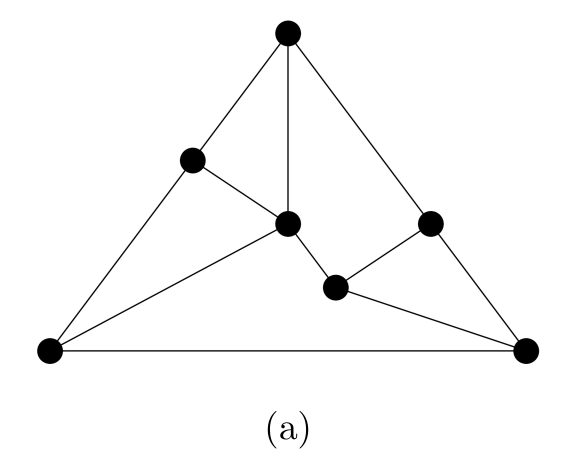
\includegraphics[width=0.3\textwidth]{Chapter 3/9. Starting graph.png}} \\ 
        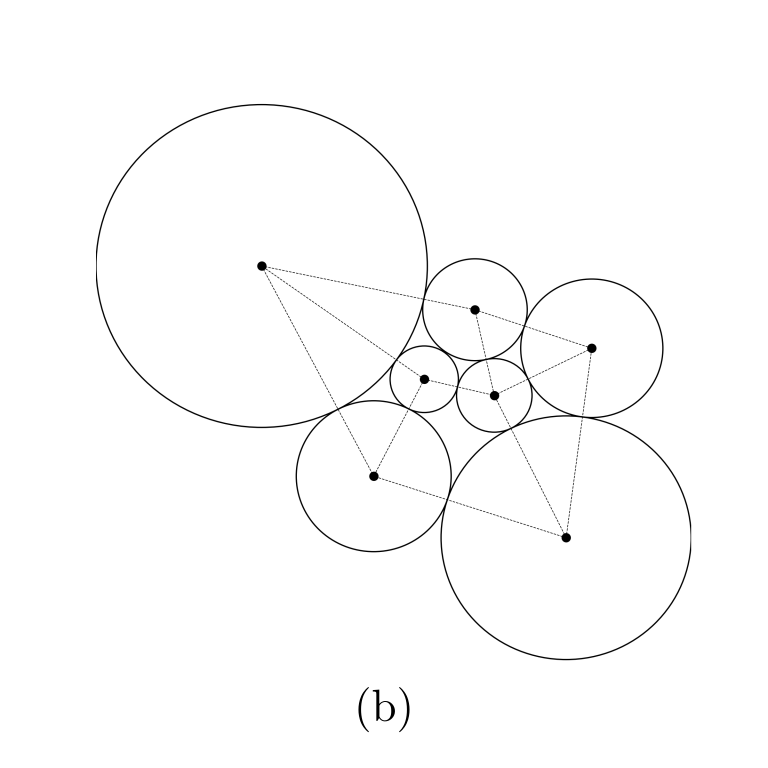
\includegraphics[width = 0.3\textwidth]{Chapter 3/10. Isomorphic packing.png} 
        & 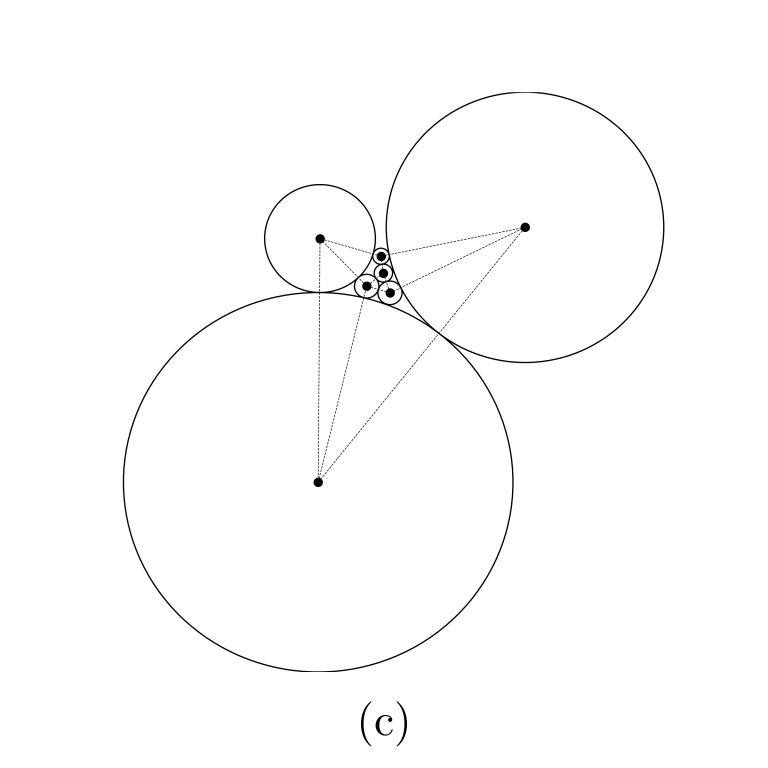
\includegraphics[width = 0.3\textwidth]{Chapter 3/11. Non-isomorphic packing.png} \\
        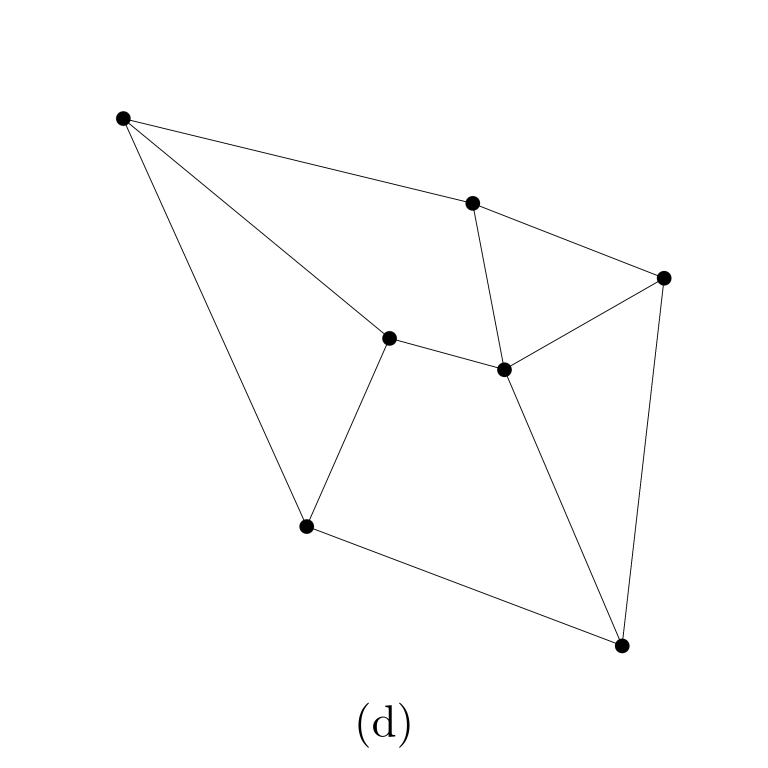
\includegraphics[width=0.3\textwidth]{Chapter 3/12. Isomorphic contact.png} &
        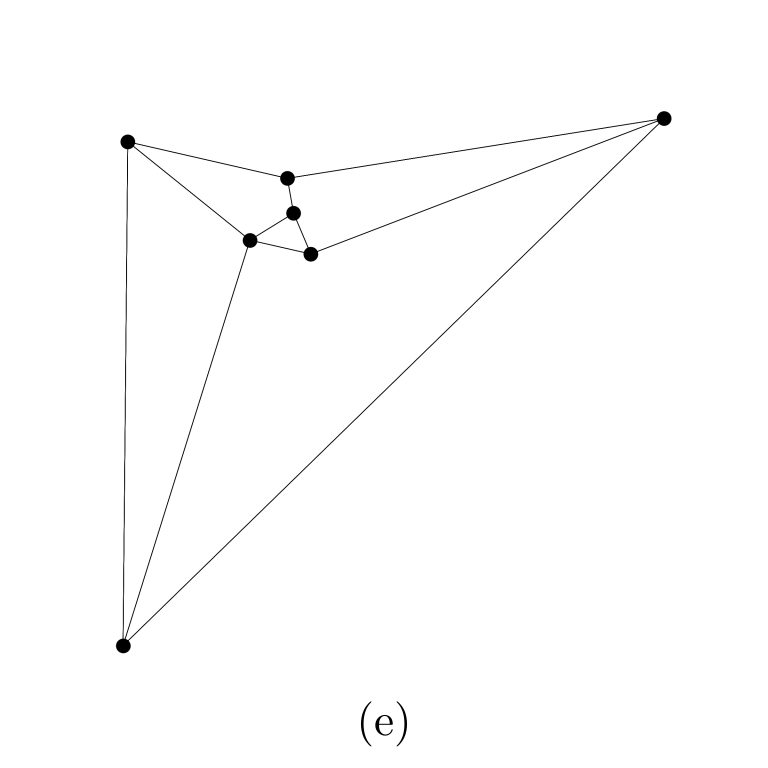
\includegraphics[width=0.3\textwidth]{Chapter 3/13. Non-isomorphic contact.png}
    \end{tabular}
    }
    \caption{A graph can have various ways in which packings can be derived from it. (a) The initial graph $G$ used to generate a circle packing. (b) A circle packing $P_1$ with a contact graph isomorphic to $G$. (c) A circle packing $P_2$ with a contact graph non-isomorphic to $G$. (d) The contact graph of $P_1$. (e) The contact graph of $P_2$.}
    \label{fig: isomorphic vs non-isomorphic packings}
\end{figure}

% lengthen the conclusion maybe?

\clearpage

%----------------------------------------------------------------------

\chapter{Minimally Rigid Graphs \& their Circle Packings} % Rigidity of Minimally Rigid Circle Packings
\label{ch: 4}

\begin{flushleft}
If we were to relate this thesis to a video game, the previous chapters would be like the levels where we, the player, would need to get through in order to `level up' and gain skills or powers. These levels would contain small challenges that we'd easily beat and gain a set of valuable tools in order to progress the game.    
\end{flushleft}

\begin{flushleft}
This chapter then, would be the showdown between the player and the final boss of the game! We'll need to call upon all of the experience gained, use every ounce of the strength developed and employ each weapon attained over the course of this journey in order to win this fight.
\end{flushleft}

\section{The Goal}

\begin{flushleft}
As it's been stated a few times leading up to this point, the project focuses on figuring out whether every minimally rigid graph has a circle packing that is infinitesimally rigid itself. It is a question for which we (currently) have no answer to, and it is an interesting one in nature because although we know that a packing such that the contact graph is isomorphic to the original graph exists by Theorem \ref{thm: circle packing theorem}, the contact graph isn't necessarily infinitesimally rigid, see Figure \ref{fig4: iso but not rig}. Our task in this chapter is to understand whether this is true or not. 
\end{flushleft}

\begin{flushleft} % argue this better
If we were to be pedantic, we would need to talk about the framework itself with respect to rigidity, and the graph which gives rise to this framework when talking about isomorphism. To avoid the confusion (and tediousness) this will cause, we shall use the words `graph' and `framework' interchangeably from now on. 
%As this chapter focuses on non-isomorphic infinitesimally rigid frameworks, we can talk about the framework itself with respect to rigidity, or the graph which gives rise to this framework when talking about isomorphism. At this stage, it does not matter which one we refer to, and therefore, we shall use the words `graph' and `framework' interchangeably. 
\end{flushleft}

\begin{figure}[htbp]
    \centering
    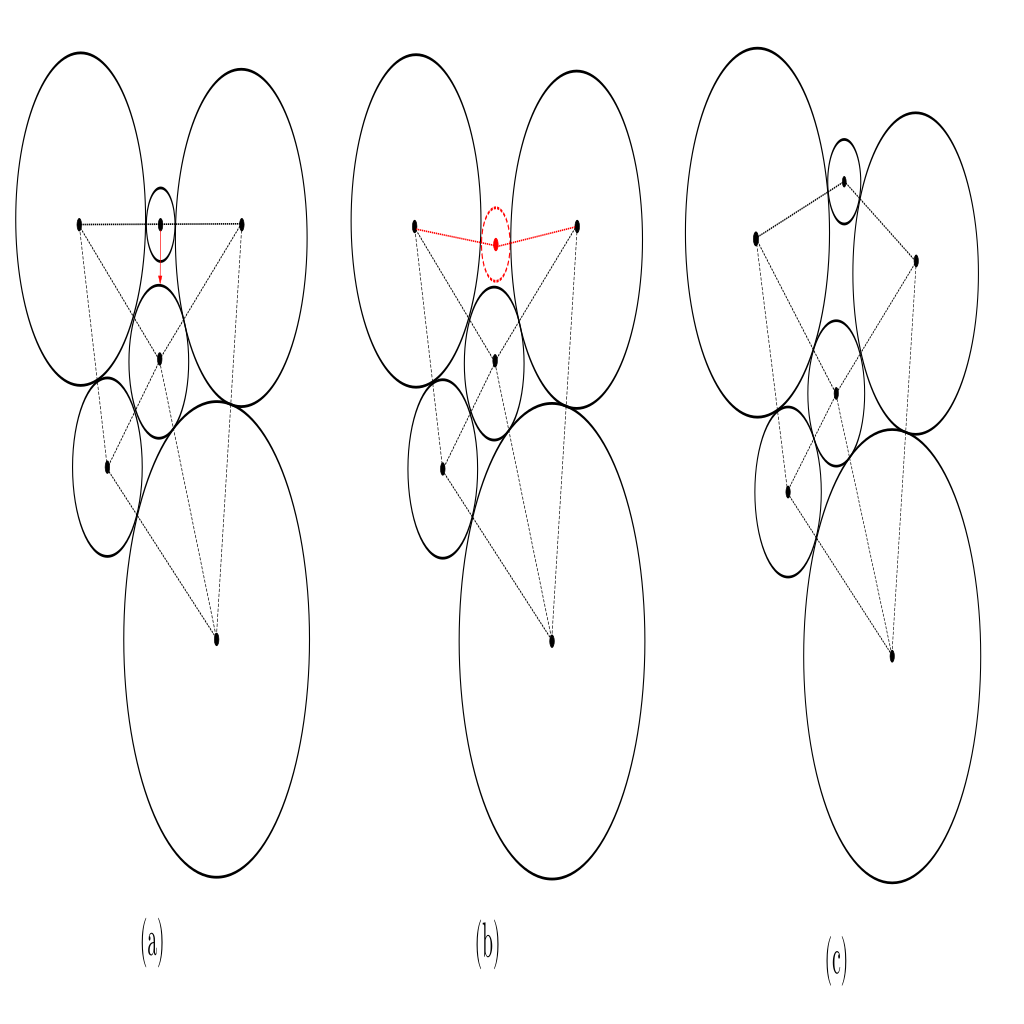
\includegraphics[width = 0.8\textwidth]{Chapter 4/2. Isomorphic but not inf rigid.png}
    \caption{Two isomorphic frameworks. (a) Can be deformed by applying instantaneous velocities (marked in red) on the inner nodes. (b) An infinitesimally rigid framework isomorphic to the one in (a).}
    \label{fig4: iso but not rig}
\end{figure}
\vspace{-3mm}
\begin{flushleft}
We try to unpack this question computationally. By finding known, non-trivial examples for which the conjecture holds, we can contemplate proving the conjecture for general cases. Thus, the two key players here are going to be modules written in Python called \texttt{Rigidity.py} and \texttt{Circle\_Packing.py}. 
\end{flushleft}

\begin{flushleft}
Titled aptly, the module \texttt{Rigidity} takes in a graph and verifies whether it is infinitesimally rigid, and \texttt{Circle\_Packing} takes a planar graph and attempts to find its circle packing using optimization methods. The graphs we'll be analyzing are all Laman graphs on $n \in [3, \hdots, 10]$ vertices.  
\end{flushleft}

\begin{flushleft}
The generation of minimally rigid graphs on $n = 3,4,5$ vertices can be easily done by hand using the Henneberg Constructions from Theorem \ref{def: henneberg}, henceforth abbreviated to $H_1$ and $H_2$ for Type I and Type II respectively. Starting with a Laman graph on 3 vertices (a triangle):
\begin{itemize}
    \item To obtain the Laman graphs on 4 vertices, we can note that applying $H_1$ yields a graph isomorphic to the one we get when applying $H_2$. so there is only one Laman graph on $4$ vertices. 
    \item To obtain the Laman graphs on 5 vertices, we apply $H_1$ to obtain three non-isomorphic graphs with 7 edges. They can be shown to be non-isomorphic by comparing the degrees of each vertex, and the cycle structure within the graph.
\end{itemize}

\noindent
This is illustrated in Figures \ref{fig4: n = 4 Laman} and \ref{fig4: n = 5 Laman}.
\end{flushleft}
\vspace{-4mm}
\begin{figure}[htbp]
    \centering
    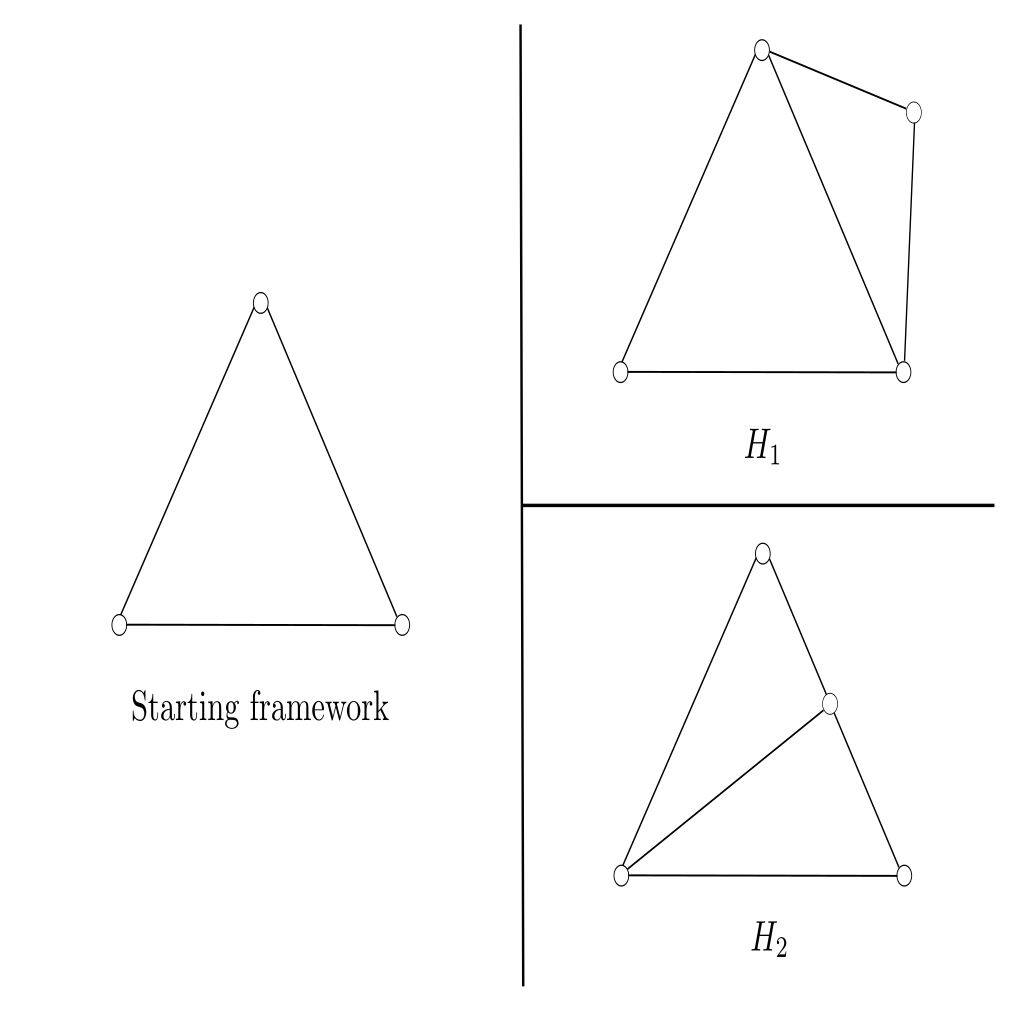
\includegraphics[width = 0.55\textwidth]{Chapter 4/3. n=4.png}
    \caption{Two isomorphic Laman graphs on 4 vertices}
    \label{fig4: n = 4 Laman}
\end{figure}

\begin{figure}[htbp]
    \centering
    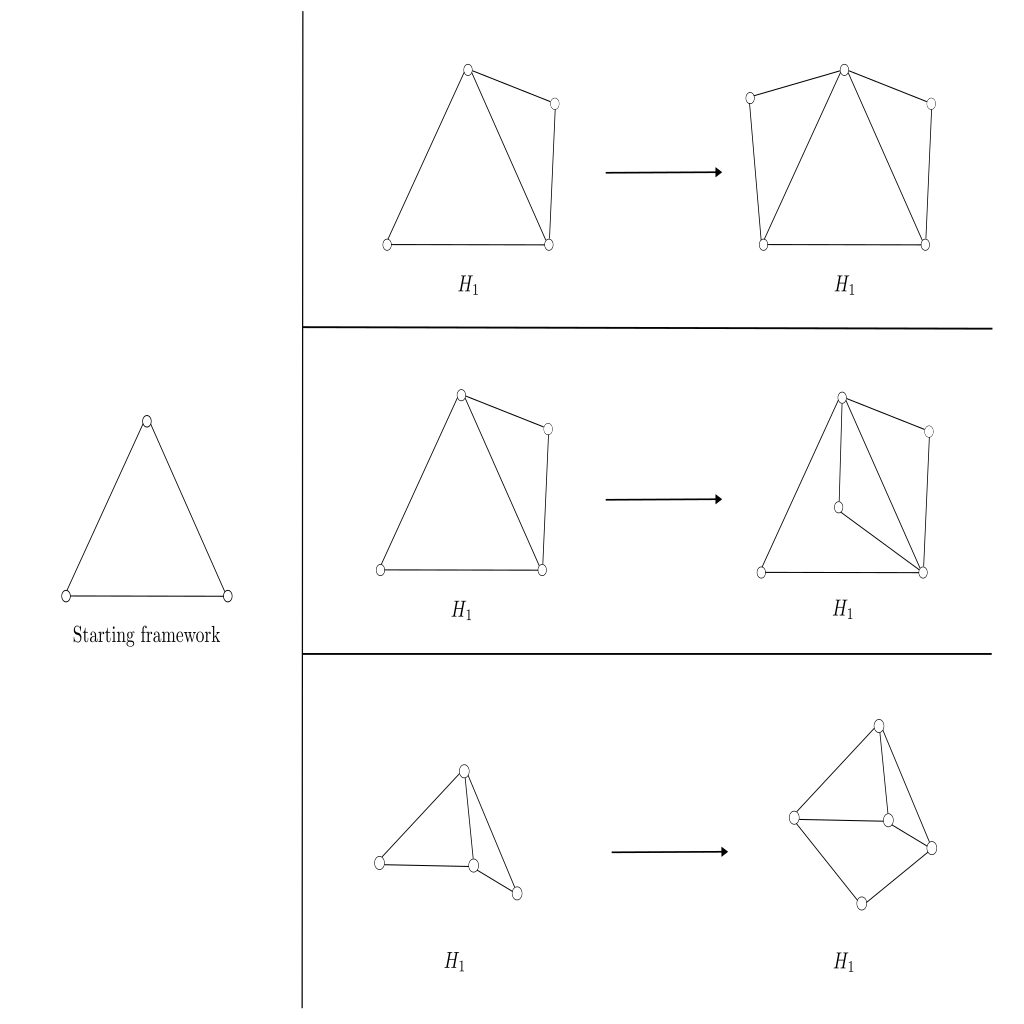
\includegraphics[width = 0.95\textwidth]{Chapter 4/4. n=5.png}
    \caption{The three non-isomorphic Laman graphs on 5 vertices}
    \label{fig4: n = 5 Laman}
\end{figure}

\begin{flushleft}
Planar graphs on vertices $n > 5$ are generated using \texttt{nauty} \cite{nauty}, which allows for the generation of non-isomorphic graphs with a specified number of vertices and edges and saves them as a \texttt{.g6} file. So for example, if we wanted to generate all planar graphs on 8 vertices with 13 edges, we would input
\end{flushleft}

\begin{center}
\texttt{./geng 8 13 | ./planarg | gzip > planar-8-13.g6}    
\end{center}

\begin{flushleft}
into the terminal. This produces a file named \texttt{planar-8-13.g6}, which contains a list of non-isomorphic planar graphs with the required vertices and edges. At this point, we would invoke the two modules \texttt{Rigidity.py} and \texttt{Circle\_Packing.py} to find the minimally rigid graphs and attempt to pack them.     
\end{flushleft}

\begin{flushleft}
    Visually, we can represent what we're trying to do in Figure \ref{fig4: config space}. For a given planar graph $G$ with $n$ vertices and $2n - 3$ edges, there can be a multitude of ways to draw frameworks for it. Referring to Figure \ref{fig4: config space}, we can visualize this as the \textit{space} of frameworks on $G$. Within this space, we have all the frameworks on $G$, some of which are infinitesimally rigid, given as blue lines.  
\end{flushleft}

\begin{figure}[htbp]
    \centering
    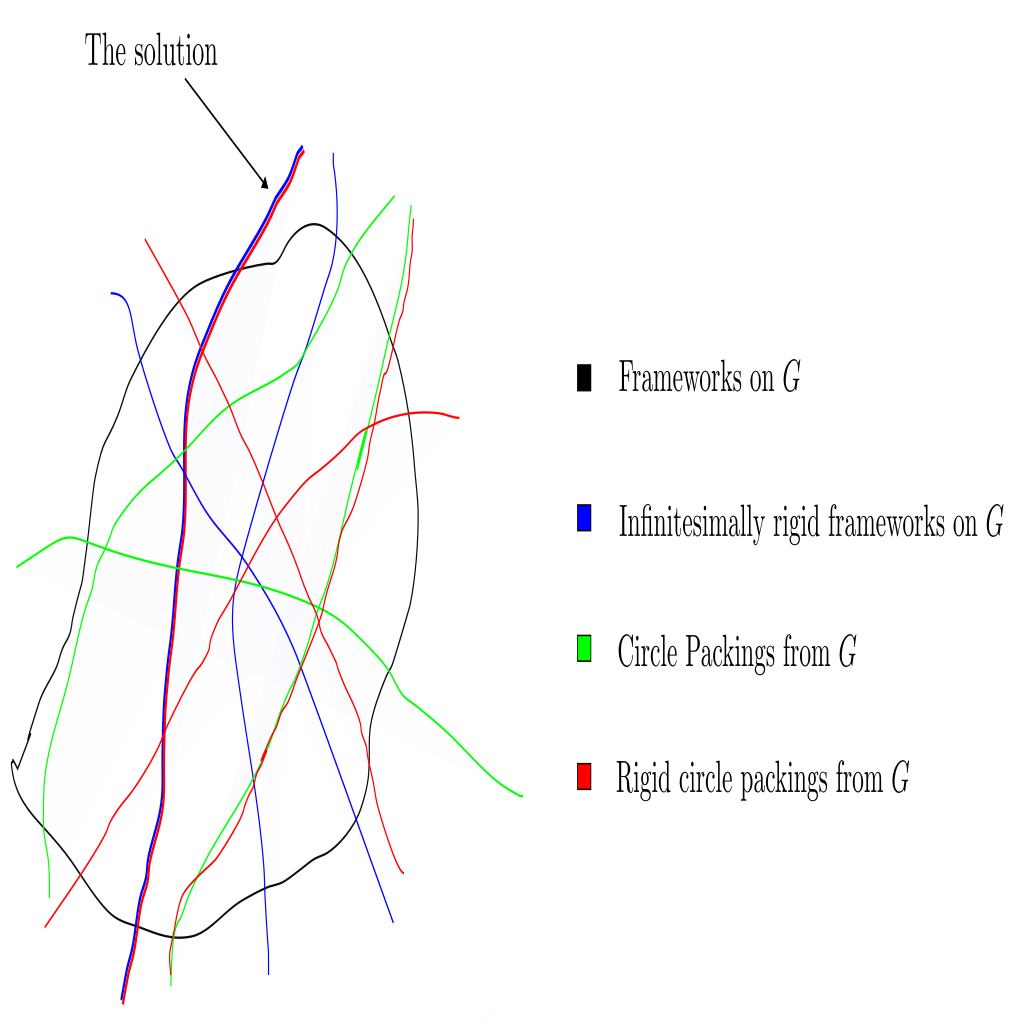
\includegraphics[width = 0.75\textwidth]{Chapter 4/5. configuration space.png}
    \caption{The space containing all frameworks on a graph $G$ drawn as a black outline, the frameworks on $G$ that are infinitesimally rigid drawn as blue lines, the circle packings obtained from $G$ drawn as green lines, and the rigid circle packings obtained from $G$ drawn as red lines.}
    \label{fig4: config space}
\end{figure}
\vspace{-4mm}
\begin{flushleft}
Now, for any circle packing obtained from $G$, its underlying contact graph could either be rigid or not, and so we have green lines to represent any circle packing we can get from $G$. Red lines are used to denote what we are after, the rigid circle packings. 
\end{flushleft}

\begin{flushleft}
Thus, the task is to find where the blue and the red lines overlap! That is, we want to find an infinitesimally rigid planar graph such that it produces a circle packing whose contact graph is also infinitesimally rigid (as this implies rigidity). Such an overlap has been made bold in the Figure. 
\end{flushleft}

\begin{flushleft}
Now that we have an understanding of what it is we're trying to do, let us dive into how we go about doing it! By exploring each module individually, we gain an understanding of what is being done. After that, we can go ahead and use the modules in order to find the packings of interest. All the code described in this chapter can be viewed on Github at \href{https://github.com/Titwik/Dissertation}{Titwik/Dissertation}.
\end{flushleft}

\section{\texttt{Rigidity.py}}

\begin{flushleft}
The first module we visit is the one we will be using to check for the rigidity of a given graph. To do this, we will need to compute the rigidity matrix from Definition \ref{def: rigidity matrix}, and then check whether its rank satisfies Theorem \ref{thm: rank-rigid}. From this point onwards, $n$ shall denote the number of vertices/nodes in a graph/framework, and $m$ shall denote the number of edges in the graph. 
\end{flushleft}

\begin{flushleft}
The graphs we will be considering are constructed using an existing module in Python known as \texttt{networkx} \cite{networkx}, allowing for the study and visualization of graphs in Python. Along with this, to create the rigidity matrix, we use a module called \texttt{numpy} \cite{numpy}. By using built-in structures and functions, such as arrays and functions related to analyzing arrays, we create the rigidity matrix as a \texttt{numpy} array and then use a function to compute its rank.
\end{flushleft}

\begin{flushleft}
This module contains several functions designed to do a particular task, so we visit each of them in turn.
\end{flushleft}

\subsection{Creating a Configuration}

\begin{flushleft}
As touched upon before, a graph is an abstract mathematical object that can be drawn in a multitude of ways. There is no concept of `distance', or the vertices having `coordinates' in $\mathbb{R}^2$. In order to study the rigidity of the graph, we must first take the vertices and give them coordinates, effectively forming a configuration of points. This brings us to the first function in this module, called \texttt{G\_configuration}.
\end{flushleft}

\begin{flushleft}
The function \texttt{G\_configuration} takes in a single argument \texttt{G}, a \texttt{networkx} graph, and begins by learning the number of vertices the graph has. For each vertex then, it randomly assigns an integer for $x$-coordinate and the $y$-coordinate from the interval $[-2^{40}, 2^{40}]$. 
Sampling for coordinates from such a large range of numbers ensures that the points are in a generic configuration, ensuring that we avoid the situation described in Figure \ref{fig: non-generic}. Finally, it returns two lists, one containing the randomly assigned $x$-coordinates and the other containing the randomly assigned $y$-coordinates.
\end{flushleft}

\begin{flushleft}
Now, we have a number of points, each equipped with their own pair of $(x,y)$ coordinates. The next step is to construct the rigidity matrix.
\end{flushleft}

\subsection{Constructing the Rigidity Matrix}

\begin{flushleft}
We define the function \texttt{rigidity\_matrix} which takes in a graph \texttt{G}, and computes its rigidity matrix with the aid of the function \texttt{G\_configuration}. Recalling Definition \ref{def: rigidity matrix}, the rigidity matrix in $\mathbb{R}^2$ has $m$ rows and $2n$ columns. Knowing this, we can initialise a \texttt{numpy} array on $m$ rows and $2n$ columns, and have every entry in the array be 0.
\end{flushleft}

\begin{flushleft}
The task at this stage is to fill in the appropriate entries of the matrix with the correct values. We use the notation $x_i$ and $y_i$ when talking about the $x$-coordinate and the $y$-coordinate of node $i$ respectively. The computation of the entries of the rigidity matrix is done by using the \texttt{enumerate} function, and we keep track of the row index \texttt{i}, as well as the edge \texttt{(u,v)} with each iteration.
\begin{enumerate}
    \item The element in row \texttt{i} and column \texttt{2u} is the $x_u - x_v$.
    \vspace{-3mm}
    \item The element in row \texttt{i} and column \texttt{2u+1} is the $y_u - y_v$.
    \vspace{-3mm}
    \item The element in row \texttt{i} and column \texttt{2v} is the $x_v - x_u$.
    \vspace{-3mm}
    \item The element in row \texttt{i} and column \texttt{2v+1} is the $y_v - y_u$.
\end{enumerate}
The function then returns the rigidity matrix with the modified elements. 
\end{flushleft}

\begin{flushleft}
To test whether this function works as expected, we can try to compute the rigidity matrix of the framework given in Example \ref{eg: rigidity matrix}. This framework has nodes with coordinates $(1,2), (0,0), (2,0)$ and $(1,1)$. 
\end{flushleft}

\begin{flushleft}
By defining the graph \texttt{G} appropriately, and by tweaking the function \texttt{rigidity\_matrix} slightly in order to take the specified coordinates rather than the random ones obtained from \texttt{G\_configuration}, we can compute the rigidity matrix for the example.
\end{flushleft}

\begin{code}
    In: print(rigidity_matrix(G))

    Out: [[ 1.  2. -1. -2.  0.  0.  0.  0.]    # edge (1,2)
          [ 0.  1.  0.  0.  0.  0.  0. -1.]    # edge (1,4)
          [-1.  2.  0.  0.  1. -2.  0.  0.]    # edge (1,3)
          [ 0.  0. -1. -1.  0.  0.  1.  1.]    # edge (2,4)
          [ 0.  0. -2.  0.  2.  0.  0.  0.]]   # edge (2,3)
\end{code}    

\begin{flushleft}
Comparing this to the rigidity matrix computed by hand in Example \ref{eg: rigidity matrix}, we see that while the order of the edges considered has changed, the entries along each corresponding row have not. Thus, we can safely say the function \texttt{rigidity\_matrix} computes the rigidity matrix for a given graph correctly.
\end{flushleft}

\subsection{Rank of the Rigidity Matrix}

\begin{flushleft}
From Theorem \ref{thm: rank-rigid}, we know that the framework is infinitesimally rigid if and only if the rank of the rigidity matrix is equal to $2n-3$. In order to obtain the rank of a matrix in Python, we make use of the \texttt{linalg} library within \texttt{numpy}. 
\end{flushleft}

\begin{flushleft}
To start, we define a function \texttt{check\_rigidity} which takes a graph \texttt{G}, and calls on the \texttt{rigidity\_matrix} function to get the rigidity matrix of \texttt{G}. From here, we use \texttt{np.linalg.matrix\_rank} to compute the rank of the matrix. If the rank is equal to $2n-3$, the function returns \texttt{True}, and \texttt{False} if the condition fails.
\end{flushleft}

\begin{flushleft}
Considering the framework in Example \ref{eg: rigidity matrix}, we know it is infinitesimally rigid by observation as it is a Laman graph on 4 vertices, and this is infinitesimally rigid by Corollary \ref{cor: laman => inf rigid}. By calling this framework \texttt{G}, let us print the rank of the rigidity matrix of \texttt{G}.
\end{flushleft}

\begin{code}
    In: print(np.linalg.matrix_rank(rigidity_matrix(G)))

    Out: 5
\end{code}

\begin{flushleft}
As $(2 \times 4) - 3 = 5$, we confirm that this framework is indeed infinitesimally rigid. Now, to verify whether \texttt{check\_rigidity} works as expected, we print its result using \texttt{G} as the argument. 
\end{flushleft}

\begin{code}
    In: print(check_rigidity(G))

    Out: True
\end{code}

\begin{flushleft}
Thus, we have written a function that now tells us whether a graph is infinitesimally rigid or not.
\end{flushleft}

\subsection{Checking rigidity for a list of graphs}

\begin{flushleft}
By using \texttt{nauty}, we create a list containing all the non-isomorphic planar graphs on a specified number of vertices and edges. Therefore, the last function this module contains is one that filters this list for all the minimally rigid graphs that we want to analyze. In addition to this, we also filter out graphs that have a vertex of degree one or two. 
\end{flushleft}

\begin{flushleft}
If a graph has a vertex with degree one, then it is not rigid and will be discarded when the \texttt{check\_rigidity} function is called. On the other hand, a vertex of degree two can be constructed using a Henneberg Type I construction, and we can pack this vertex by simply creating a circle tangent to two other circles. It is a trivial process and for this reason, such graphs are not very interesting to look at.
\end{flushleft}

\begin{flushleft}
We start defining the function \texttt{find\_rigid\_graphs} by allowing the argument to be a list of graphs. As this list contains graphs, each with the same number of vertices, we choose the first graph in the list and let $n$ be the number of vertices in this graph. 
\end{flushleft}

\begin{flushleft}
In order to filter out the graphs containing a vertex of degree of two, we first loop through all the graphs in the list, and then loop through each vertex in each graph. If the graph does \textbf{not} contain a vertex with degree two, then we add it to a separate list called \texttt{graphs\_without\_degree\_2}. 
\end{flushleft}

\begin{flushleft}
From here, we loop through all the graphs in \texttt{graphs\_without\_degree\_2}, check its rigidity using \texttt{check\_rigidity}, and add it to a new list called \texttt{rigid\_graphs}. Finally, the function \texttt{find\_rigid\_graphs} returns \texttt{rigid\_graphs}, a list containing all planar minimally rigid graphs of minimum degree at least three.
\end{flushleft}

\subsection{Testing the code}

\begin{flushleft}
The last thing to do is to ensure that the code works for known examples before we start investigating graphs we know nothing about. Graphs that are not infinitesimally rigid can be seen in Figures \ref{eg: not_rigid} and \ref{eg: not inf rigid 2.0}. For an additional graph that is known to be infinitesimally rigid, we consider the Framework in Figure \ref{eg: inf rigid}. We label these graphs \texttt{G1}, \texttt{G2} and \texttt{G3} respectively, and construct them using \texttt{networkx}.
\end{flushleft}

\begin{figure}[htbp]
    \centering
    \begin{tabular}{c c c}
        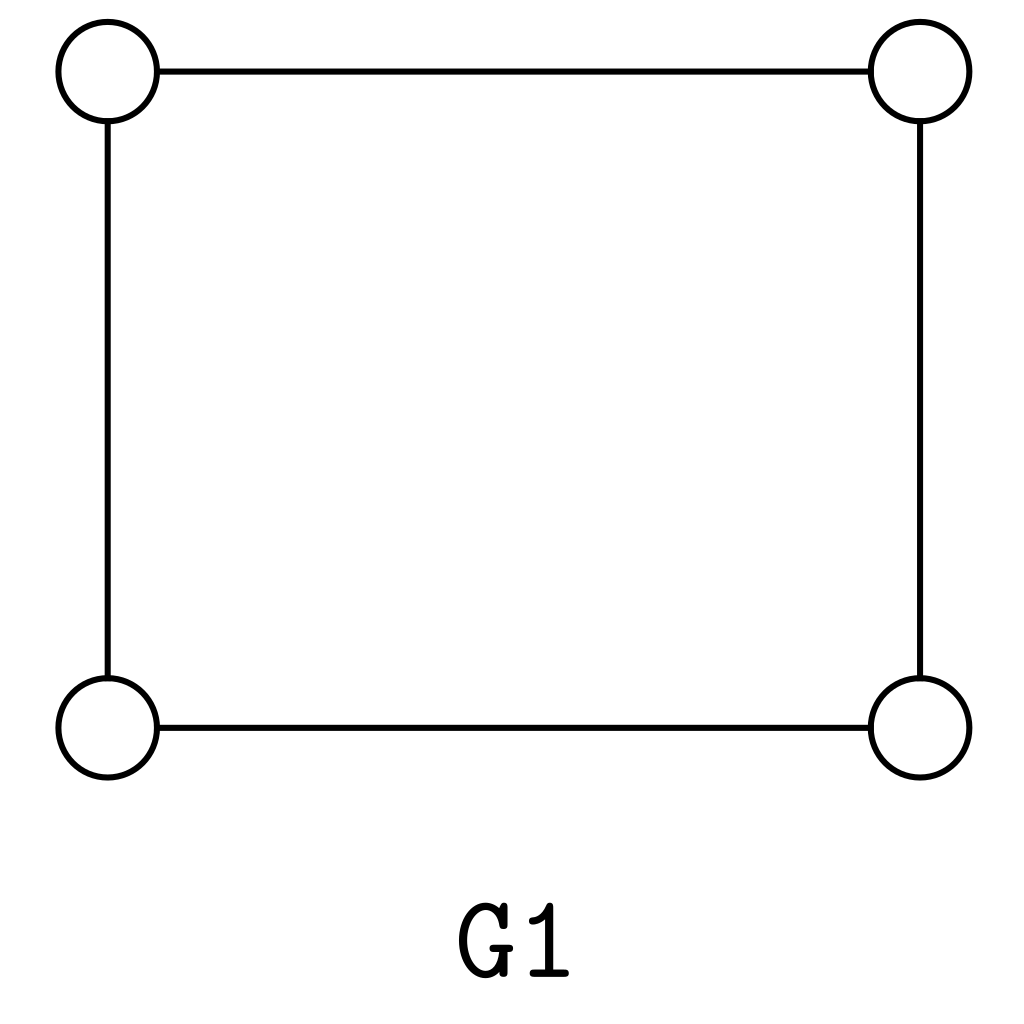
\includegraphics[width = 0.25\textwidth]{Chapter 4/6. not_rigid.png} 
        & 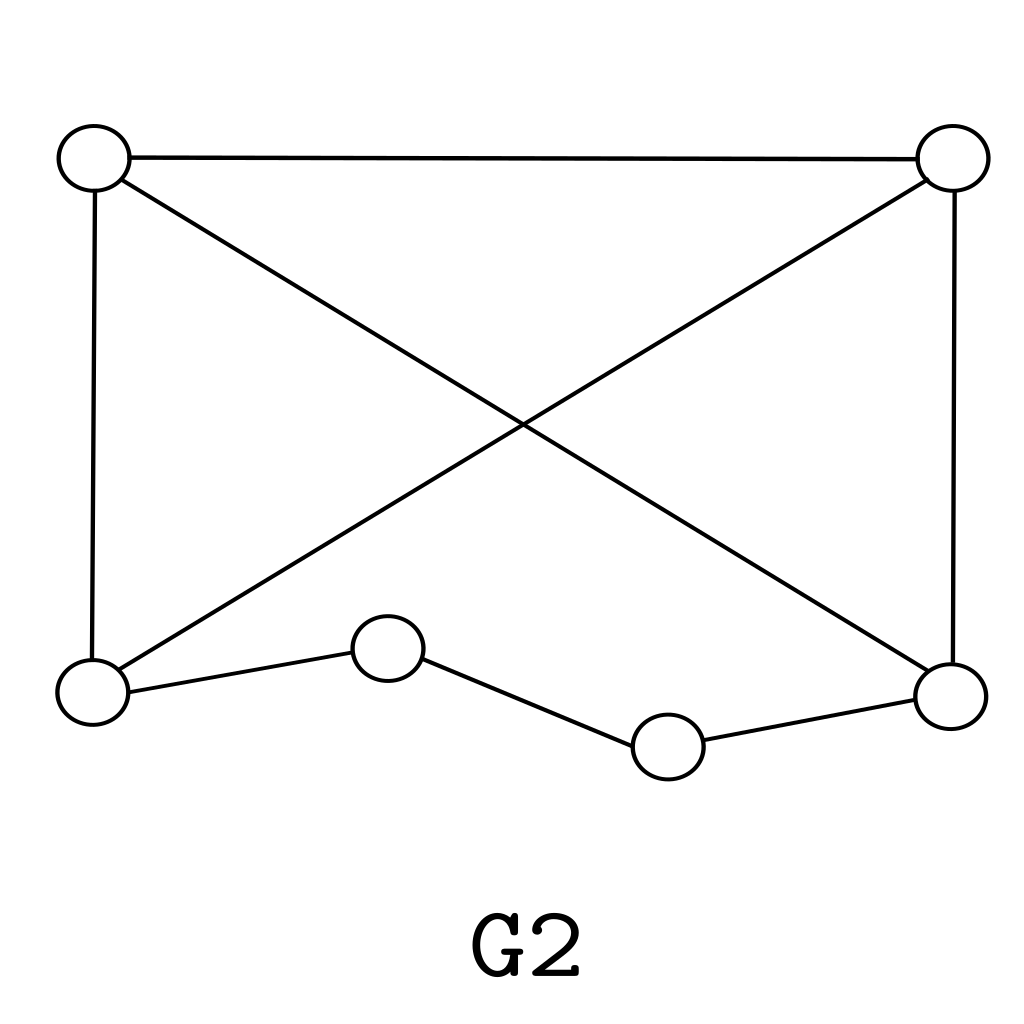
\includegraphics[width = 0.25\textwidth]{Chapter 4/7. not_inf_rigid_2.0.png} &
        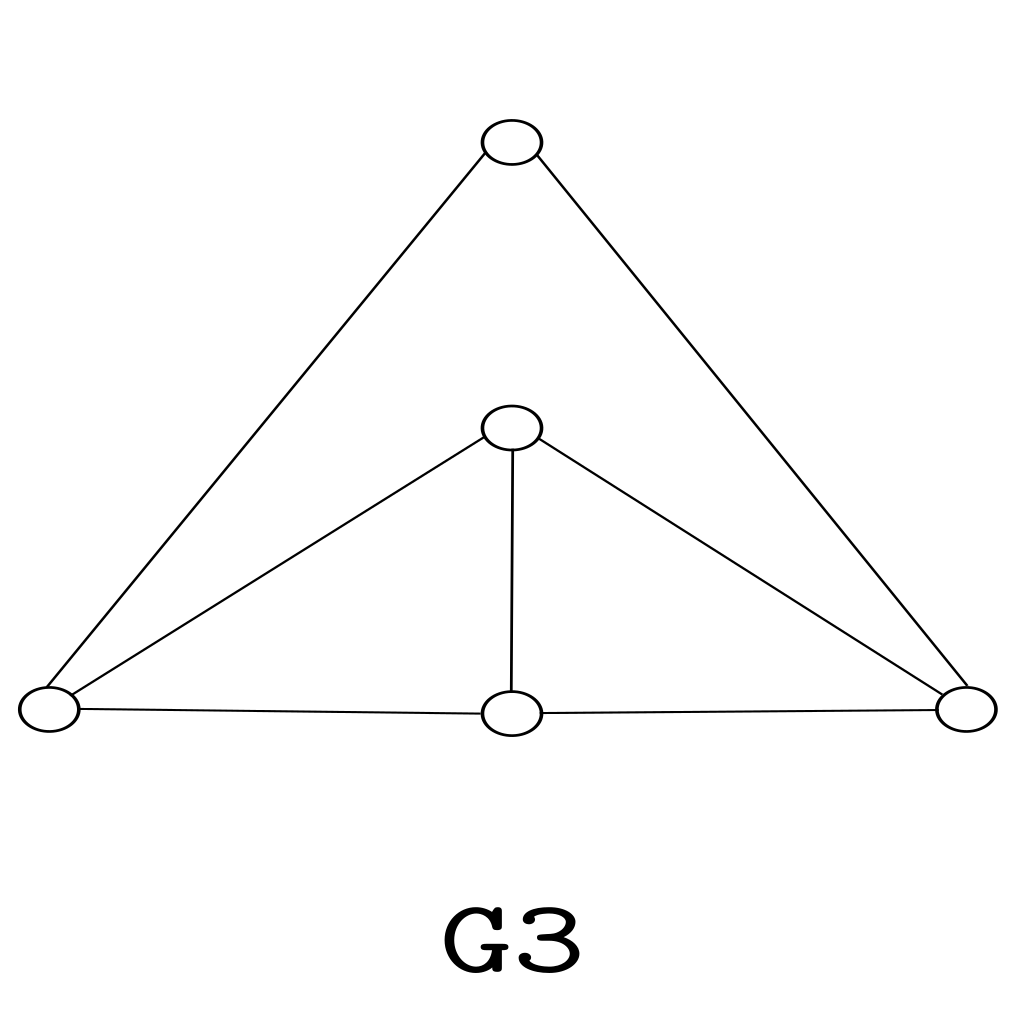
\includegraphics[width=0.2\textwidth]{Chapter 4/8. inf_rigid.png}        
    \end{tabular}
    \caption{The frameworks from Figures \ref{eg: not_rigid}, \ref{eg: not inf rigid 2.0} and \ref{eg: inf rigid} labelled as \texttt{G1}, \texttt{G2}, and \texttt{G3} respectively.}
\end{figure}

\begin{code}
    In [1]: print(check_rigidity(G1))
    Out: False 
    
    In [2]: print(check_rigidity(G2))
    Out: False
    
    In [3]: print(check_rigidity(G3))
    Out: True
\end{code}

\begin{flushleft}
This is reassuring to see! We've successfully verified that the functions work well with each other, and that their outputs are as expected. So, we can confidently identify infinitesimally rigid graphs, and can move onto creating circle packings for a given planar graph. 
\end{flushleft}

\section{\texttt{Circle\_Packing.py}}

\begin{flushleft}
The process of finding circle packings for a graph involves a process called \textit{numerical minimization}. It is a method in which we try to minimize the variables involved in a given problem subject to clearly defined rules or \textit{constraints}. In order to find circle packings, we first have to define the problem carefully through an \textit{objective function}, impose certain constraints, generate a `guess' of what the solution might be, and then feed this information into a minimizer. Let us briefly run through exactly what this module covers. 
\end{flushleft}

\begin{flushleft}
It is made up of four functions, each performing a specific task, similar to how the functions were defined in \texttt{Rigidity.py}. 
\begin{enumerate}
    \item The first of these functions defines the objective function that we want to minimize.
    \vspace{-3mm}
    \item The second function imposes the constraints that the minimization process should obey. 
    \vspace{-3mm}
    \item The third function generates a random list of initial conditions for the coordinates of every node in the framework, as well as randomly generated radii for the circles they inhabit.
    \vspace{-3mm}
    \item The very last function is one that uses the three previous functions in order to generate a circle packing for a graph.
\end{enumerate}
\end{flushleft}

\begin{flushleft}
The minimizer that we will be using comes from the \texttt{scipy} \cite{scipy} library in Python called \texttt{scipy.optimize.minimize}, which we refer to as \texttt{minimize} from now on. To illustrate how this minimizer works, let us do a simple example.
\end{flushleft}

\subsection{Using the Minimizer: A Simple Example}

\begin{flushleft}
Suppose we have a rectangle of length $x$ and width $y$, and we wish to maximize its area $xy$, subject to the constraint that its perimeter is 20 units. Translating this into something that we can use in the minimizer, the objective function would be $-xy$ as we are trying to maximize the area with the minimize function. The constraint can be modelled as $2x+2y = 20$ and our initial guesses for the values of $x$ and $y$ could be 6 and 4 respectively. 
\end{flushleft}

\begin{flushleft}
We would input this into the \texttt{minimize} function, and obtain the optimal values of $x$ and $y$ satisfying these constraints such that the area of the rectangle is maximized. The code for this example is shown below.
\end{flushleft} 

\begin{code}
    # define the objective function
    def area_rectangle(xy):
        x = xy[0]
        y = xy[1]
        area = xy[0] * xy[1]
        return -area
    
    # define the constraint
    cons = ({`type':`eq', `fun': lambda xy: 2*xy[0] + 2*xy[1] - 20})
    
    # define the initial condition, where 6 is our initial x value and 
    # 4 is our initial y value
    initial_guess = [6,4]
    
    # use the minimizer
    result = scipy.optimize.minimize(area_rectangle, initial_guess, constraints = cons)
\end{code}

\begin{code}
    In: print(f"x = {result.x[0]} and y = {result.x[1]}")
    Out: x = 5.0 and y = 5.0    
\end{code}

\begin{flushleft}
Therefore, the values of $x$ and $y$ that maximize the area of a rectangle with a perimeter of 20 units are 5 and 5 respectively. Hopefully this example provides some insight into how we can leverage the minimizer. We will not be delving too deep into how the \texttt{minimize} works at this stage, but understanding how to use it properly is imperative for when we attempt to find a circle packing for a graph.
\end{flushleft}

\begin{flushleft}
With that in mind, let us dive into the first function in the \texttt{Circle\_Packing.py} module!
\end{flushleft}

\subsection{Creating the Objective Function}

\begin{flushleft}
Let $(G, \mathbf{p})$ be a framework, $x_i$ and $y_i$ be the $x$-coordinate and $y$-coordinate of node $i$, and $r_i$ be the radius of the circle this node inhabits. We consider the node to be the center of this circle.
\end{flushleft}

\subsubsection{Defining the objective function}

\begin{flushleft}
To begin constructing the function that we wish to minimize, we first consider the distance between two nodes and set it equal to the sum of the radii of the circles they inhabit. That is;

\begin{equation*}
    (x_i - x_j)^2 + (y_i-y_j)^2 = (r_i + r_j)^2 \hspace{16mm} \forall i,j \in V(G)    
\end{equation*}

\vspace{2mm}
When using the minimizer however, we must input this equation such that the right hand side must be equal to 0. Therefore, we write this as 

\begin{equation*}
    (x_i - x_j)^2 + (y_i-y_j)^2 - (r_i + r_j)^2 = 0 \hspace{10mm} \forall i,j \in V(G)
\end{equation*}

\vspace{2mm}
As we saw in the example above, by trying to minimize a negative objective function, we end up maximizing it instead. To avoid such complications arising in this scenario, we square the entire function so that the values we work with are strictly positive.

\begin{equation*}
    ((x_i - x_j)^2 + (y_i-y_j)^2 - (r_i + r_j)^2)^2 = 0 \hspace{11mm} \forall i,j \in V(G)
\end{equation*}

\vspace{2mm}
At this stage, we will have several equations, one for each pair of nodes. The final step to obtain the objective function will be to consider the sum of all these equations. Therefore, the function that we treat as our objective function will be 

\begin{equation}\label{eq:circle_constraint}
    \sum_{\substack{i,j=1 \\ i \neq j}}^{n} \left( (x_i - x_j)^2 + (y_i - y_j)^2 - (r_i + r_j)^2 \right)^2
  \end{equation}
\end{flushleft}

\subsubsection{Writing the code}

\begin{flushleft}
To input Equation \ref{eq:circle_constraint} as the objective function into the minimizer, we first define a function \texttt{mk\_obj} that takes in a graph \texttt{G}, and construct another function named \texttt{objective\_function} within this function like so;
\end{flushleft}

\begin{code}
    # function that returns the objective function
    def mk_obj(G):
        
        # create a function that computes the objective function of a graph G
        def objective_function(vars):
        ...
\end{code}

\begin{flushleft}
The argument \texttt{vars} represents a list of the variables \texttt{[x1,y1,r1, ... , xn,yn,rn]}. These are the variables that will be minimized when we use the minimizer, where \texttt{xi} and \texttt{yi} represent the $x$-coordinate and $y$-coordinate respectively of node $i$, and \texttt{ri} is the radius of the circle this node centers.
\end{flushleft}

\begin{flushleft}
Inside \texttt{objective\_function}, we define three new functions, \texttt{x(i)}, \texttt{y(i)} and \texttt{r(i)}:

\begin{enumerate}
    \item The function \texttt{x(i)} returns \texttt{vars[3*i]}.
    \vspace{-3mm}
    \item The function \texttt{y(i)} returns \texttt{vars[3*i+1]}.
    \vspace{-3mm}
    \item The function \texttt{r(i)} returns \texttt{vars[3*i+2]}.
\end{enumerate}

For example, the $x$-coordinate of every node occurs in positions 0, 3, 6, ..., in \texttt{vars}, and so the function \texttt{x(i)} returns every third element of \texttt{vars}. The remaining two functions are definined similarly.
\end{flushleft}

\begin{flushleft}
Lastly, we initialise a variable \texttt{total} to store the sum of the objective functions, and set it to 0. Looping through all the edges $(i,j) \in E(G)$, we compute the sum given in Equation \ref{eq:circle_constraint}, and return this sum as follows;
\end{flushleft}

\begin{code}
    # initialise a sum
    total = 0
    
    # compute the sum 
    for (i,j) in G.edges():
        total += ((x(i) - x(j)) ** 2 + (y(i) - y(j)) ** 2 - (r(i) + r(j)) ** 2) ** 2
    
    # return the sum
    return total
\end{code}

\begin{flushleft}
All that's left to do is to return the output of the \texttt{objective\_function} as the output of \texttt{mk\_obj}.
\end{flushleft}

\begin{code}
    def mk_obj(G):
        def objective_function(vars):
            ...
            return total
        return objective_function
\end{code}

\begin{flushleft}
This completes the function \texttt{mk\_obj}, a function that takes in a graph, and returns its objective function. By feeding this into the minimizer, we are essentially telling the computer to make each variable in the list \texttt{vars} as small as they can be. The next step we will need to take is informing the minimizer of the constraints that should be obeyed.
\end{flushleft}

\subsection{Defining the Constraints}

\begin{flushleft}
The constraints can be thought of rules that the minimizer must follow. In our case, to generate a circle packing such as the one in Figure \ref{fig: circle packing example}, the constraints we impose are:

\begin{enumerate}
    \item Each circle must have a positive radius.
    \vspace{-3mm}
    \item Each circle must have a maximum radius.
    \vspace{-3mm}
    \item The circles must not overlap or contain each other.
\end{enumerate}

To present these constraints to the minimizer, we code each one carefully, add it to a list named \texttt{constraints}, and then feed this list to the minimizer. By adhering to these rules, the minimizer will produce a configuration of circles, each equipped with a radius, such that the conditions required for a circle packing are satisfied. We begin by creating a function \texttt{cons}, which takes a graph \texttt{G} as its argument, and tackle each constraint mentioned in the list above individually.
\end{flushleft}

\subsubsection{1. Each circle must have a positive radius.}

\begin{flushleft}
To ensure that the radius is positive, we set a tolerance value \texttt{epsilon} such that the radius must be at least \texttt{epsilon}. Setting this tolerance as 0 is not possible as it leads to a host of problems due to the nature of floating point arithmetic (which we will not discuss any further). 
\end{flushleft}

\begin{flushleft}
Choosing an appropriate tolerance can be challenging as if it were too big, then we disallow circles of very small radii to be formed, which may not converge to a circle packing. On the other hand, picking a value too small can lead to numerical instability due to the nature of optimization, as well as increase the time it takes for the minimizer to converge to a solution.
\end{flushleft}

\begin{flushleft}
After some trial and error, letting \texttt{epsilon = 0.04} strikes the balance of achieving accurate circle packings in a reasonable duration of time. To enter the constraint in a format the minimizer will accept, we first loop through every vertex in \texttt{G}, indexed by \texttt{i}, and write the constraint as 
\end{flushleft}

\begin{code}
    # radius must be greater than epsilon constraint
    {`type': `ineq', `fun': lambda vars, i=i: vars[3*i + 2] - epsilon}
\end{code}

\begin{flushleft}
Let us consider each term in this entry individually:

\begin{itemize}
    \item (\texttt{`type': `ineq'}) means that the constraint that we are entering is an inequality.
    \vspace{-3mm}
    \item (\texttt{`fun': lambda vars, i=i}) means that the function we are using is one named \texttt{lambda}, and this function takes in arguments \texttt{vars} and \texttt{i}.
    \vspace{-3mm}
    \item (\texttt{vars[3*i + 2] - epsilon}) is the inequality $r_i > \epsilon$ that we use to define positive radii. As the right hand side must be 0, we consider the inequality $r_i - \epsilon > 0$.
\end{itemize}

We then add this to the list \texttt{constraints}, and move onto the next constraint we wish to impose. 
\end{flushleft}

\subsubsection{2. Each circle must have a maximum radius.}

\begin{flushleft}
We set a maximum radius to ensure computational efficiency, and also prevent the creation of excessively large circles that could obscure the other circles present in the packing. This guarantees that all circles are visible and the arrangement remains visually appealing. 
\end{flushleft}

\begin{flushleft}
Here, the maximum radius chosen will be 10 units, and is implemented as a constraint by looping through every vertex in \texttt{G}, indexed by \texttt{i}. Adding
\end{flushleft}

\begin{code}
    {`type': `ineq', `fun': lambda vars, i=i: 10 - vars[3*i + 2]}
\end{code}

\begin{flushleft}
to the list \texttt{constraints}, we continue to write the final constraint we need to implement.
\end{flushleft}

\subsubsection{3. The circles must not overlap or contain each other.}

\begin{flushleft}
By implementing the two constraints above, we have guaranteed the existence of circles in our packing. However, there is nothing stopping a circle from extending over into another circle's interior. This also includes the scenario where one circle lies completely within another circle. From Definition \ref{def: circle packing}, we know that each circle must either be tangential with another, or have nothing to do with each other.
\end{flushleft}

\begin{flushleft}
In order to achieve this, we set a final constraint such that the distance between any two nodes in $G$ must be at least the sum of the radii of the circles they center. This can be written as

\[
(x_i - x_j)^2 + (y_i - y_j)^2 \geq (r_i + r_j)^2
\]

\vspace{2mm}
for all $i,j \in V(G)$ such that $i \neq j$. Then when we have equality, the circles with centers $(x_i, y_i)$ and $(x_j, y_j)$ are tangential. Otherwise, the circles do not interact.
\end{flushleft}

\begin{flushleft}
We do this by first looping through all the vertices in \texttt{G}, indexed by \texttt{i}, and nesting another loop through the vertices of \texttt{G}, this time indexed by \texttt{j}. As we only want to consider pairs of vertices $(i,j)$ where $i \neq j$, we set an \texttt{if} condition to achieve this. Thus, we add this constraint to our list \texttt{constraints} as;
\end{flushleft}

\begin{code}
    {`type': `ineq', `fun': lambda vars, i=i, j=j: 
    (vars[3*i] - vars[3*j])**2 + (vars[3*i + 1] - vars[3*j + 1])**2 - 
    (vars[3*i + 2] + vars[3*j + 2])**2}
\end{code}

\begin{flushleft}
which allows us to secure a packing where the circles are tangential and their interiors are disjoint! The \texttt{cons} function now returns the list \texttt{constraints} containing the three rules we want our packing to obey. 
\end{flushleft}

\begin{flushleft}
So far, we have our objective function and a list of constraints that the circle packing should stick to. The very last thing that we need before we can invoke the minimizer is a list of initial conditions for the coordinates of each node in the graph, as well as for each radius in the circle packing.
\end{flushleft}

\subsection{Generating Initial Conditions}

\begin{flushleft}
The initial conditions will be generated using a function we define as \texttt{initial\_conditions}, which takes a graph \texttt{G} as an argument. To do this, we make use of the \texttt{random} \cite{random} module in Python. By using a random configuration each time the \texttt{initial\_conditions} function is called, we ensure that the minimizer gets a new place to start from. Doing it this way bypasses the situation where we get stuck trying to pack a configuration known to fail repeatedly.
\end{flushleft}

\begin{flushleft}
We allow the initial $x$ and $y$ coordinates to be obtained from the continuous range $[0,10]$, and the radius $r$ will have initial radii generated from the range $[0,1]$. By choosing a small interval for the initial coordinates of each node, if the initial configuration of points closely matches a circle packing, then we can expect the minimizer to arrive there quickly.
\end{flushleft}

\begin{flushleft}
To start generating the coordinates and radii, we begin by creating a list \texttt{IC}, and then loop through all the nodes in \texttt{G}. For each node, we generate an $x$ and $y$ coordinate using the function \texttt{random.uniform(0,10)} to draw a random number between 0 and 10 uniformly. For each radius $r$, we use \texttt{random.uniform(0,1)} to draw a random number between 0 and 1 uniformly.
\end{flushleft}

\begin{flushleft}
We insert each randomly generated number into \texttt{IC} in the order [$x,y,r$], to match with the variable \texttt{vars} from before. The function \texttt{initial\_variables} finally returns \texttt{IC}, a list containing $n$ initial $x$-coordinates, $n$ initial $y$-coordinates, and $n$ initial radii, totalling $3n$ elements in the list.
\end{flushleft}

\begin{flushleft}
Summarizing everything we have so far, for a given graph \texttt{G}, we have defined functions that take in \texttt{G} and return the objective function that is to be minimized, a list of constraints to adhere to in order to form a circle packing, and a list of initial conditions for the coordinates of each circle's center, as well as their radii. The last step to take is to use the minimizer in order to obtain the circle packing for a planar graph.
\end{flushleft}

\begin{flushleft}
Before we do this though, let's take a quick detour and go through some fundamental ideas of numerical optimization, the issues that arise during minimization, and what we can do to overcome these issues. 
\end{flushleft}

\subsection{Detour: Understanding Optimization}

\begin{flushleft}
The aim of this section is to learn a little bit about what happens behind the scenes when we use the \texttt{minimize} function. In particular, how the initial conditions chosen play a big role in the convergence to a solution. As an example, let us go through how the initial conditions affect the root-finding abilities of the Newton-Raphson method.
\end{flushleft}

\subsubsection{Example: Newton-Raphson Method}

\begin{flushleft}
The Newton-Raphson method is an algorithm used to find the roots $x_r$ of a given function $f(x)$. It is used as follows:
\begin{enumerate}
    \item Pick an initial $x = x_0$, and compute its corresponding $f(x_0)$.
    \vspace{-3mm}
    \item Draw the tangent of $f(x)$ at the point $x = x_0$, and mark the tangent's intersection with the $x$-axis as $x_1$.
    \vspace{-3mm}
    \item Repeat steps 1 and 2 by setting $x_0 = x_1$ until the algorithm converges to $x_r$.
\end{enumerate}

This is shown in Figure \ref{fig: newton}. Clearly, with an increasing number of iterations, our values for $x = x_i$ converge towards the root $x_r$. However, this is dependent on the function $f(x)$, as well as the initial position $x=x_0$ chosen, see Figure \ref{fig: bad newton}. 
\end{flushleft}

\begin{figure}[htbp]
    \centering
    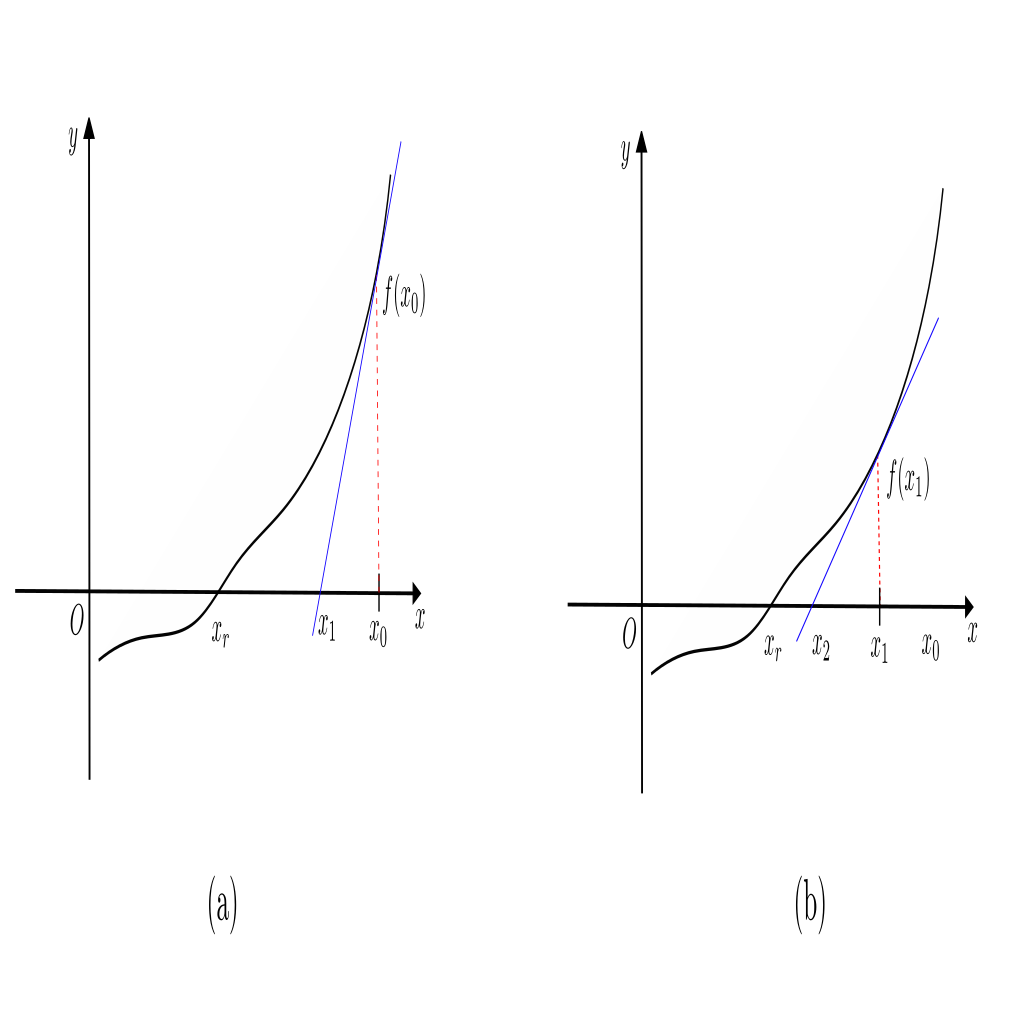
\includegraphics[width = 1\textwidth]{Chapter 4/9. newton raphson.png}
    \caption{(a) First iteration of the Newton-Raphson Method. (b) Second iteration of the Newton-Raphson Method.}
    \label{fig: newton}
\end{figure}

\begin{figure}[htbp]
    \centering
    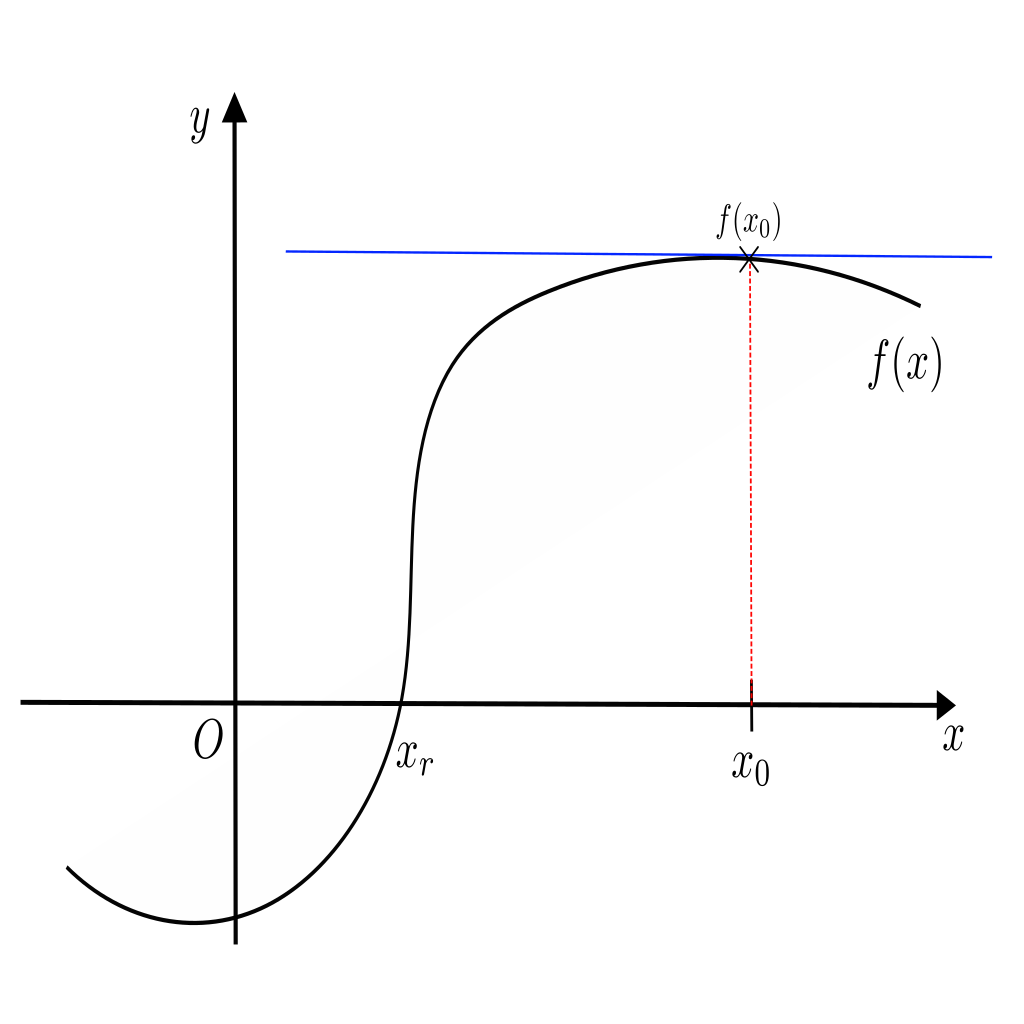
\includegraphics[width = 0.5\textwidth]{Chapter 4/10. bad newton raphson.png}
    \caption{A poorly chosen initial $x=x_0$. The tangent (blue line) will not intersect the $x$-axis anywhere near the root $x_r$.}
    \label{fig: bad newton}
\end{figure}

\vspace{-4mm}
\begin{flushleft}
These two examples showcase how the convergence to a solution can be extremely sensitive to the initial conditions chosen. Choose well, and we converge to the solution ($x_r$ in this case) quickly, but if our initial condition is chosen poorly, the convergence may be significantly delayed or may not occur at all.
\end{flushleft}

\subsubsection{Global vs Local Minimum}

\begin{flushleft}
An additional factor that can prevent us from obtaining a correct circle packing is when the minimizer reaches a \textit{local} minimum, and not the \textit{global} minimum. A circle packing is achieved if only if the minimizer converges to the global minimum. 
\end{flushleft}

\begin{figure}[htbp]
    \centering
    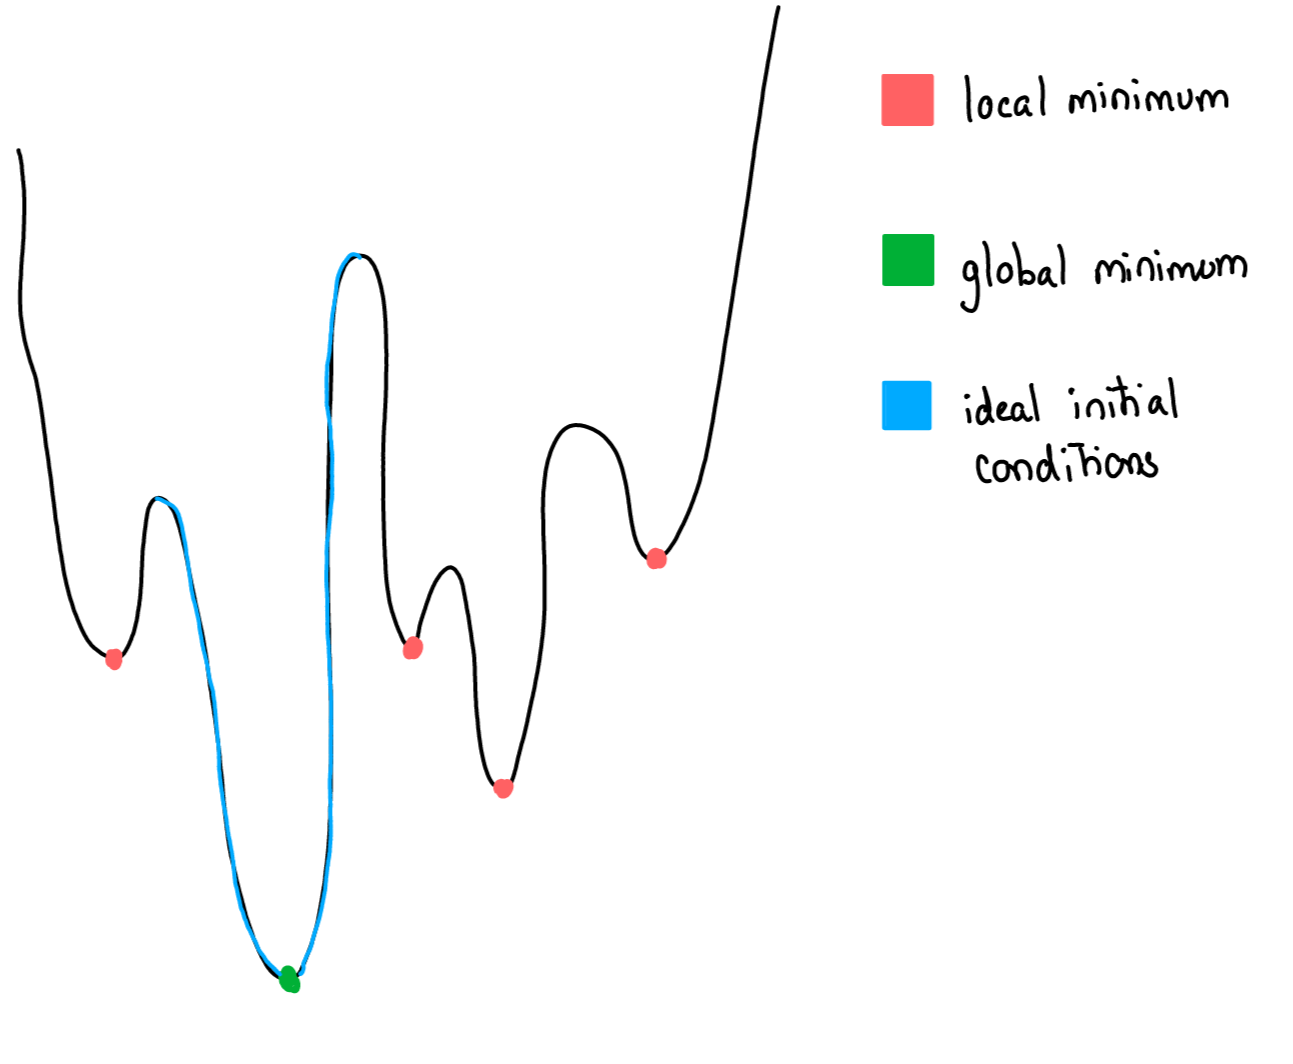
\includegraphics[width = 0.5\textwidth]{Chapter 4/11. energy.png}
    \caption{A visualization of the local minimums and the global minimum the minimizer can achieve. To achieve the global minimum, the initial condition must be along the slopes leading down to the global minimum.}
    \label{fig4: minimum}
\end{figure}

\vspace{-4mm}
\begin{flushleft}
Initial conditions play a part in achieving a global minimum as well. Consider Figure \ref{fig4: minimum}, and suppose we have an initial condition that is placed on one of the slopes descending towards a local minimum (given as red dots). 
\end{flushleft}

\begin{flushleft}
If the minimizer were to start here, then it would minimize the objective function until it reaches a local minimum, believe that it has reached the global minimum, and then return a false solution. Therefore, the ideal initial condition must be on the the slope going down to the global minimum (given as blue slopes).
\end{flushleft}

\subsubsection{Overcoming pitfalls}

\begin{flushleft}
Such a situation can be tricky to navigate. Are we always able to pick suitable initial conditions such that the minimizer attains the global minimum? Moreover, how do we verify that it is indeed at a global minimum? Such questions can be hard to answer in general, but thankfully in our case, we can use some of the tools picked up along the way to aid us!
\end{flushleft}

\begin{flushleft}
The first thing we do is verify whether the minimizer hits a global or local minimum. We know that a correct circle packing is generated when the minimizer achieves a global minimum. Additionally, we know from Definition \ref{def: contact graph} that since our graph $G$ has $2n-3$ edges, the circle packing obtained must also have $2n-3$ contacts. 
\end{flushleft}

\begin{flushleft}
Therefore, we can verify that the minimizer attains a global minimum if and only if the resulting circle packing has $2n-3$ contacts! 
\end{flushleft}

\begin{flushleft}
If the minimizer produces a circle packing that doesn't have $2n-3$ contacts, then this means the initial conditions were unfavorable and it converged to a local minimum. In this case, we call the function \texttt{initial\_conditions}, generating a new random configuration of points and radii, and attempt to pack the graph once more. 
\end{flushleft}

\begin{flushleft}
Armed with the knowledge to combat situations in which the minimizer arrives to an incorrect solution, we embark on the final stretch to complete this module. 
\end{flushleft}

\subsection{Finding Circle Packings}

\subsubsection{Using the minimizer}

\begin{flushleft}
We begin the search for a circle packing of a given graph \texttt{G} by first defining a function \texttt{circle\_packing}, which takes \texttt{G} as an argrument. From here, start a \texttt{while} loop and call the \texttt{minimize} function like so;
\end{flushleft}

\begin{code}
    result = minimize(mk_obj(G), initial_conditions(G), 
                        constraints = cons(G), method='COBYLA')
\end{code}

\begin{flushleft}
where the first argument is the objective function of \texttt{G} we minimize, the second is the list of initial conditions for the configuration of nodes and radii, the third is the list of constraints imposed, and the last argument defines the method of optimization used (Constrained Optimization BY Linear Approximations, or COBYLA)\footnote{should i explain why this method? doesnt seem important}. 
\end{flushleft}

\begin{flushleft}
The list \texttt{result.x} contains all the minimized variables, and recalling how the variable \texttt{vars} was defined in the \texttt{mk\_obj} function, we know that they are stored in the order \texttt{[x1,y1,r1, ..., xn,yn,rn]}. After the \texttt{minimize} function achieves a minimum, we retrieve the $x$ and $y$ coordinates along with the radii $r$ by creating three new lists named \texttt{x\_list}, \texttt{y\_list}, \texttt{r\_list}, looping through \texttt{result.x}, and sorting each element into one of the three lists. 
\end{flushleft}

\begin{flushleft}
For example, the $x$-coordinates are saved in \texttt{x\_list} by;
\end{flushleft}

\begin{code}
    x_list = []

    for i in range(n):
        x = result.x[3*i]
        x_list.append(x)
\end{code}

\subsubsection{Testing for a global minimum}

\begin{flushleft}
Before we use these variables to display a circle packing, we need to make sure that the minimizer achieved a global minimum and not a local one, which happens if the circle packing contains $2n-3$ contacts. We verify this by looping through every pair of coordinates $(x_i,y_i)$, where $x_i$ and $y_i$ are the $x$ and $y$ coordinates of node $i$ respectively, and check whether the the distance between two nodes equals the sum of the radii of their respective circles. We expect $2n-3$ such equalities.
\end{flushleft}

\begin{flushleft}
Initializing a \texttt{counter} with initial value 0, and a \texttt{tolerance} for 0 as 0.001, we check the number of contacts by;
\end{flushleft}

\begin{code}
    for i in range(n):
            x1 = x_list[i]
            y1 = y_list[i]

            for j in range(i+1,n):
                x2 = x_list[j]
                y2 = y_list[j]

                # check if the distance between the centers is equal to the sum of radii
                if abs(np.sqrt((x1 - x2) ** 2 + (y1 - y2) ** 2) - 
                            (r_list[i] + r_list[j])) < tolerance:
                    counter += 1  # add one to the counter
\end{code}

\begin{flushleft}
We continue the code under the \texttt{if counter == (2*n - 3)} condition, as we have a successful packing if this is satisfied. If this condition fails, the loop restarts and the \texttt{minimize} function is called again with a new configuration of points and radii. 
\end{flushleft}

\subsubsection{Creating the contact graph}

\begin{flushleft}
In preparation for the analysis of the circle packings generated, we generate the contact graph of the successful packing as a \texttt{networkx} graph. This done in a very similar fashion to how we checked for $2n-3$ contacts.
\end{flushleft}

\begin{flushleft}
We start by initializing an empty \texttt{networkx} graph called \texttt{contact\_graph}, and if circles centered by nodes $i$ and $j$ are tangential, then we add an edge between nodes $i$ and $j$ in the contact graph. Doing this for every node in the circle packing produces the contact graph of the packing, which will be used later on.
\end{flushleft}

\subsubsection{Generating the circle packing}

\begin{flushleft}
Here, we will be generating three different figures named \texttt{fig1}, \texttt{fig2} and \texttt{fig3}. 
\begin{itemize}
    \item \texttt{fig1} will be the circle packing.
    \vspace{-3mm}
    \item \texttt{fig2} will be the circle packing with its contact graph visualized within the packing.
    \vspace{-3mm}
    \item \texttt{fig3} will be the contact graph of the circle packing. 
\end{itemize}

Let's begin drawing circles!\footnote{do i need the details on how i plotted and scaled the circle packing?}
\end{flushleft}

\begin{flushleft}
We initialize \texttt{fig1}, along with its axis \texttt{ax1} using \texttt{fig1, ax1 = plt.subplots()}. From here, we start a loop over \texttt{n}, the number of nodes in the graph \texttt{G}, and index this loop using \texttt{i}. Recall that the coordinates of the circles in the packing are stored in lists \texttt{x\_list} and \texttt{y\_list}, while the radii are stored in \texttt{r\_list}. We set the variables \texttt{x,y} and \texttt{r} as \texttt{x\_list[i], y\_list[i]}, and  \texttt{r\_list[i]} respectively. Using the \texttt{circle} function from the \texttt{matplotlib} library, we plot the circle with center \texttt{(x,y)} and radius \texttt{r} in \texttt{fig1}. Doing this for every set of coordinates and radii completes the circle packing in \texttt{fig1}.
\end{flushleft} 

\begin{flushleft}
For \texttt{fig2}, we repeat the process done in \texttt{fig1} to plot the same circle packing, with the additions of a visible center and a dashed line between the centers of tangential circles. Finally, \texttt{fig3} drops the plotting of the circles but keeps the plot of the contact graph generated within the packing, as done in \texttt{fig2}.
\end{flushleft}

\begin{flushleft}
At the very end, the function \texttt{circle\_packing} returns the original graph \texttt{G}, the \texttt{networkx} contact graph of the packing \texttt{contact\_graph}, and the figures \texttt{fig1}, \texttt{fig2} and \texttt{fig3}. This completes the module \texttt{Circle\_Packing.py}!
\end{flushleft}

\subsubsection{Testing the code}

\begin{flushleft}
As with the \texttt{Rigidity.py} module, we must test the function \texttt{circle\_packing} on known examples before we venture out into the unknown. The graphs we use to test will be the Laman graphs on three and four vertices and five vertices, see Figures  \ref{fig4: n = 4 Laman} and \ref{fig4: n = 5 Laman}. Although these graphs have vertices of degree 2, this does not matter for testing purposes. 
\end{flushleft}

\begin{flushleft}
We can construct the circle packing for each of these graphs easily, and then compare them to what the \texttt{circle\_packing} function returns. This is done in Figures \ref{fig4: 4 node packing} and \ref{fig4: 5 node packing}. The left column contains packings done by hand, and the right column contains the corresponding circle packing generated using the function \texttt{circle\_packing}.
\end{flushleft}

\begin{figure}[htbp]
    \centering      
    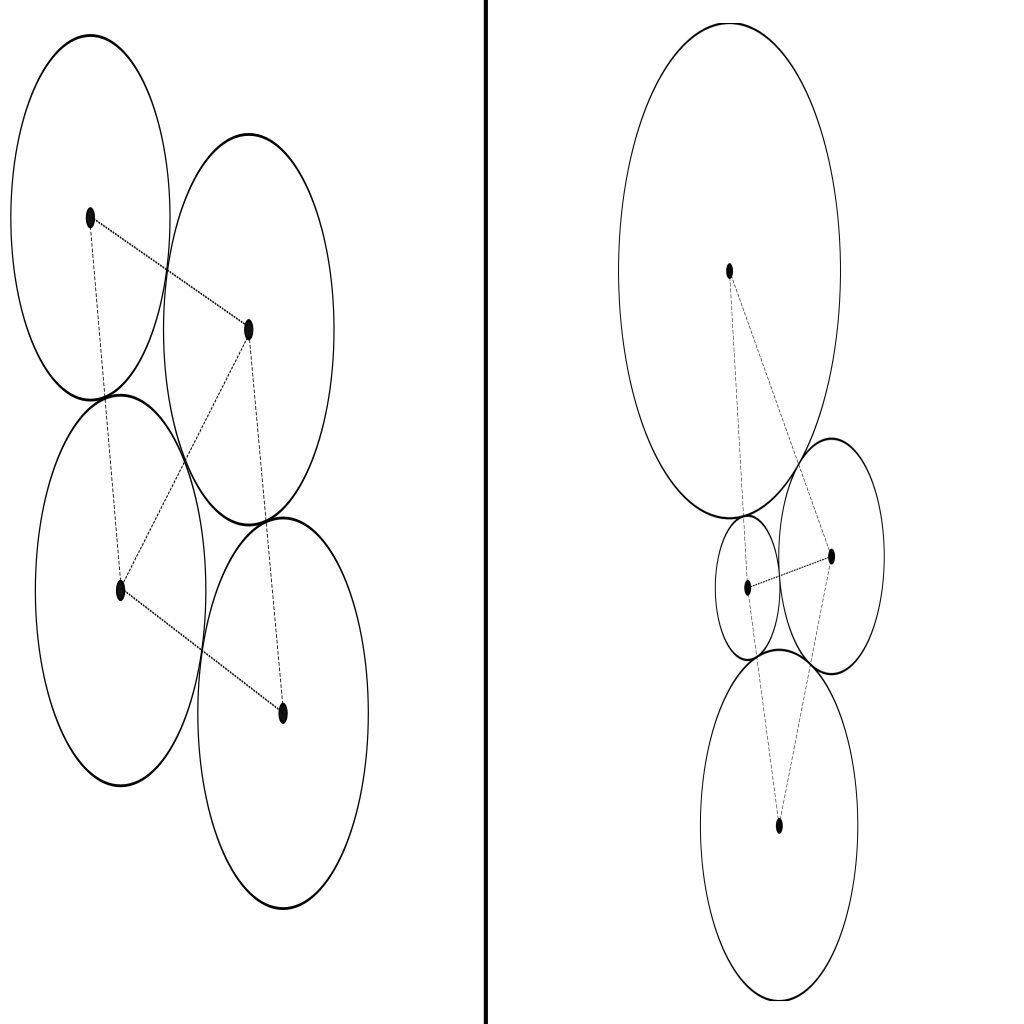
\includegraphics[width = 0.7\textwidth]{Chapter 4/12. 4 circle.png} \hspace{1 cm}
    \caption{Circle packing for the Laman graph on 4 nodes seen in Figure \ref{fig4: n = 4 Laman}. Left: drawn by hand. Right: generated using \texttt{circle\_packing}.} 
    \label{fig4: 4 node packing}
\end{figure}

\begin{figure}[htbp]
    \centering
    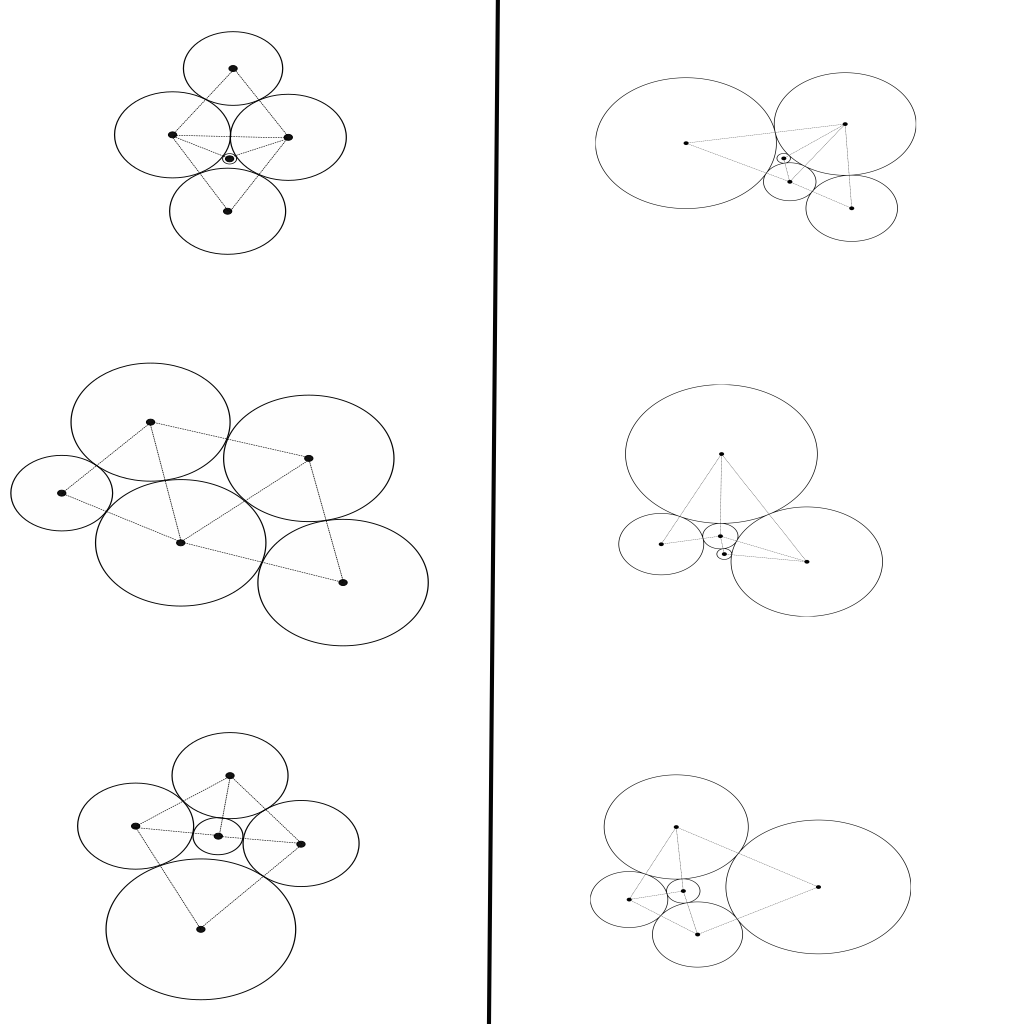
\includegraphics[width = 0.7\textwidth]{Chapter 4/13. 5 circle.png}
    \caption{Circle packings for the Laman graphs on 5 nodes seen in Figure \ref{fig4: n = 5 Laman}. Left column: drawn by hand. Right Column: generated using \texttt{circle\_packing}.}
    \label{fig4: 5 node packing}
\end{figure}

\begin{flushleft}
With these results, we confirm that the code developed in this module successfully finds a circle packing for a given planar graph.
\end{flushleft}

\section{Investigating the Conjecture}

\begin{flushleft}
To remind ourselves of what the conjecture is, we write it here once more:

\begin{center}
    \textit{``For every planar and minimally rigid graph, does there exist a circle packing that is also infinitesimally rigid?''}
\end{center}

Taking stock of everything we have;
\begin{itemize}
    \item Using \texttt{nauty}, we generated a list of non-isomorphic planar graphs with $n$ vertices and $2n-3$ edges.
    \vspace{-3mm}
    \item With the \texttt{Rigidity.py} module, we filter the list of planar graphs for minimally rigid ones with minimum degree 3.
    \vspace{-3mm}
    \item Using the \texttt{Circle\_Packing.py} module, we are able to generate the circle packing for a planar graph.
\end{itemize}

Therefore, our plan of attack will follow Algorithm 4.1.
\end{flushleft}
\begin{flushleft}
\textbf{Algorithm 4.1:} \footnote{use code language instead of plain english?}
\begin{enumerate}
    \item Generate a list of planar graphs on $n$ vertices using \texttt{nauty}.
    \vspace{-3mm}
    \item Use \texttt{find\_rigid\_graphs} from \texttt{Rigidity.py} and filter the list for minimally rigid planar graphs on $n$ vertices and minimum degree 3. Call this list \texttt{rigid\_graphs}.
    \vspace{-3mm}
    \item Initialize variables \texttt{attempt = 0}, \texttt{position = 0} and \texttt{max\_attempt = 500}.
    \vspace{-3mm}
    \item While \texttt{True}:
    \vspace{-3mm}
    \begin{enumerate}
        \item Increment \texttt{attempt} by 1.
        \vspace{-1mm}
        \item Call \texttt{circle\_packing} from \texttt{Circle\_Packing.py} for \texttt{rigid\_graphs[position]}.
        \vspace{-1mm}
        \item If the contact graph of the packing is isomorphic to \texttt{rigid\_graphs[position]} \textbf{\underline{and}} \texttt{check\_rigidity(contact\_graph)} returns \texttt{True} \textbf{\underline{and}} \texttt{position} is less than the length of \texttt{rigid\_graphs}:
        \begin{enumerate}
            \item Save \texttt{G}, \texttt{contact\_graph} \texttt{fig1}, \texttt{fig2} and \texttt{fig3}.
            \vspace{-1mm}
            \item Increment \texttt{position} by 1.
            \vspace{-1mm}
            \item Set \texttt{attempt} to 0.
        \end{enumerate}
        \vspace{-1mm}
        \item Else if the contact graph of the packing is isomorphic to \texttt{rigid\_graphs[position]} \textbf{\underline{and}} \texttt{check\_rigidity(contact\_graph)} returns \texttt{True} \textbf{\underline{and}} \texttt{position} is equal to the length of \texttt{rigid\_graphs}:
        \begin{enumerate}
            \item Save \texttt{G}, \texttt{contact\_graph} \texttt{fig1}, \texttt{fig2} and \texttt{fig3}.
            \vspace{-1mm}
            \item \texttt{break} out of the loop
        \end{enumerate}
        \vspace{-1mm}
        \item Else if the contact graph of the packing is not isomorphic to \texttt{rigid\_graphs[position]}, \textbf{\underline{or}} \texttt{check\_rigidity(contact\_graph)} returns \texttt{False}, \textbf{\underline{and}} \texttt{attempt} is equal to \texttt{max\_attempt}:
        \begin{enumerate}
            \item print ``Max attempts done, no viable packing found. Code terminating''
            \vspace{-1mm}
            \item \texttt{break} out of the loop
        \end{enumerate}
    \end{enumerate}
\end{enumerate}
\end{flushleft}

\begin{flushleft}
This algorithm is implemented in a script named \texttt{Rigid\_Packings.py}, and was used to verify whether all minimally rigid planar graphs on $n \in [3, \hdots, 10]$ have circle packings such that they are infinitesimally rigid. Therefore, it is possible to confirm that confirm that all minimally rigid planar graphs on $n \in [3, \hdots, 9]$ satisfy the conjecture. However, the code written here has displayed a few limitations, which we are going to address now.
\end{flushleft}

\subsection{Limitations to the code}

\subsubsection{1. Huge differences in radii}

\begin{flushleft}
When Algorithm 4.1 was implemented to one of the minimally rigid graphs on 9 nodes, the code failed to produce a circle packing after 500 attempts. Let this graph be known as $G$, and it is shown in Figure \ref{fig4: interesting}.
\end{flushleft}

\begin{figure}[htbp]
    \centering
    \begin{tabular}{c | c}
        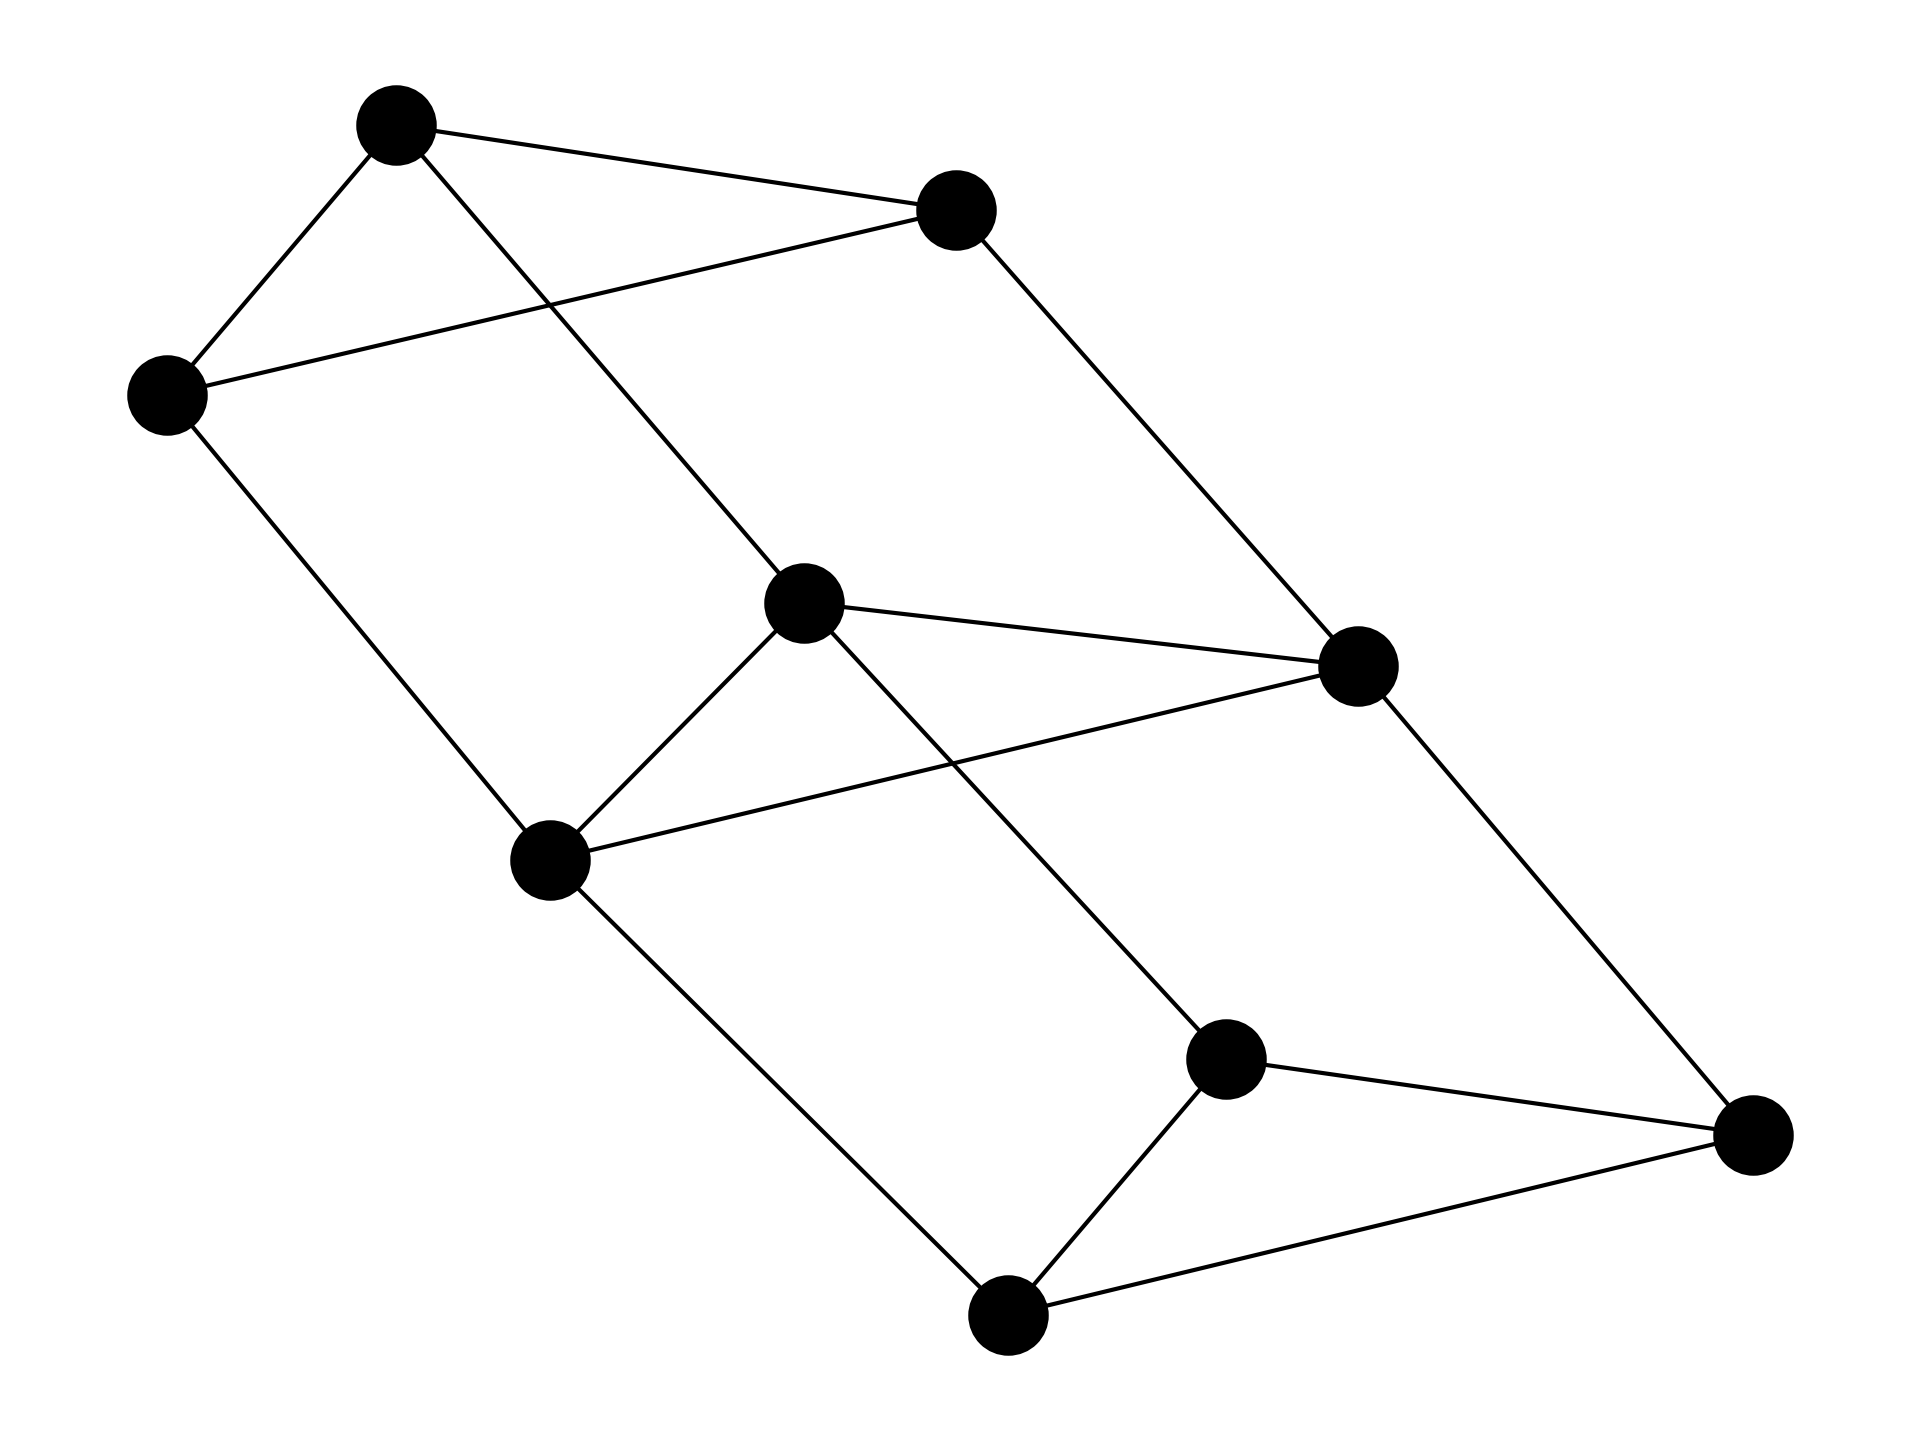
\includegraphics[width = 0.4\textwidth]{Chapter 4/14. interesting graph.png} & \hspace{5 mm} 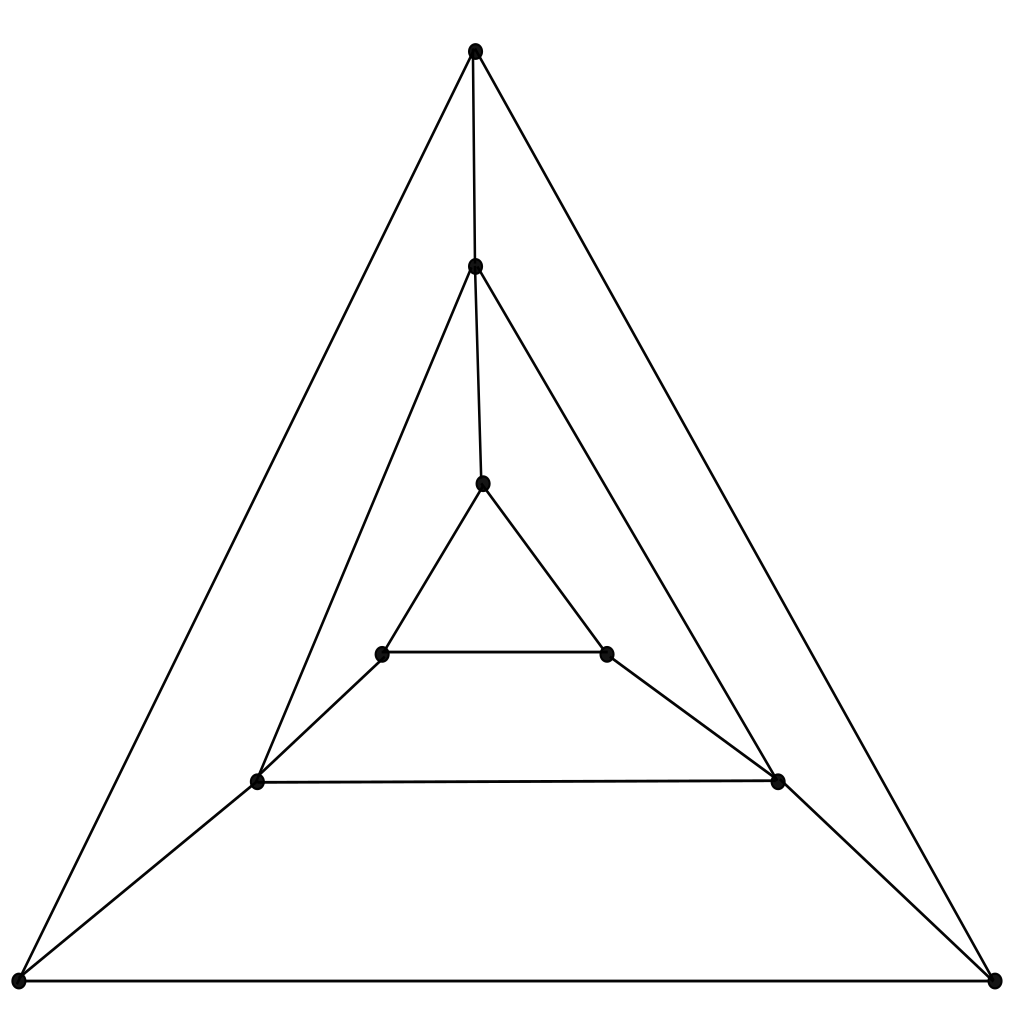
\includegraphics[width = 0.3\textwidth]{Chapter 4/15. interesting planar.png}   
    \end{tabular}
    \caption{Left: The graph $G$ that could not be packed computationally. Right: The planar vizualization of this graph}
    \label{fig4: interesting}
\end{figure}

\begin{flushleft}
Upon further investigation, it can be shown that this graph has a circle packing such that its contact graph is isomorphic to $G$. This is shown in Figure \ref{fig4: interesting packing}. As we can see, there is a vast difference between the radius of the largest circles on the `outside', and the inner-most circles. 
\end{flushleft}

\begin{figure}[htbp]
    \centering
    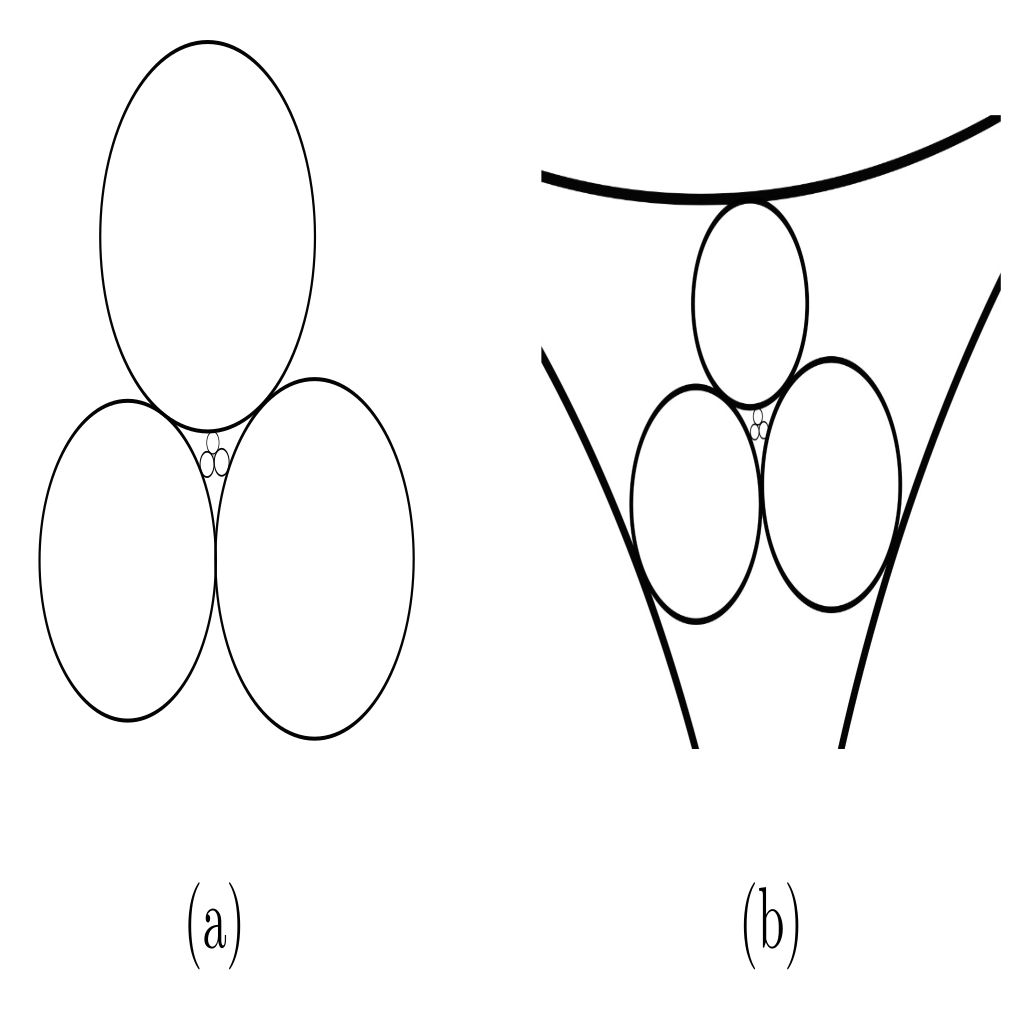
\includegraphics[width = 0.5\textwidth]{Chapter 4/16. interesting circle packing.png}
    \caption{(a) The circle packing for $G$. (b) The packing zoomed into the center to show the inner-most circles.}
    \label{fig4: interesting packing}
\end{figure}

\vspace{-5mm}
\begin{flushleft}
It is believed that due to this large difference in radii, the minimizer finds it difficult to place the circles correctly. This was tested by setting initial conditions in a configuration that matches the circle packing shown in Figure \ref{fig4: interesting packing}, but even then, the minimizer failed to provide the correct packing. 
\end{flushleft}

\begin{flushleft}
We can thereby conclude that even if an appropriate circle packing does exist for a graph, we may not be able to achieve it if the (absolute) difference between the biggest radius and the smallest radius in the packing is large. 
\end{flushleft}

\subsubsection{2. The initial conditions for increasing $n$}

\begin{flushleft}
The keen reader may have noticed that earlier, it was mentioned that Algorithm 4.1 was used to test minimally rigid graphs on $n \in [3, \hdots, 10]$ vertices, and that we can confirm the conjecture for $n \in [3, \hdots, 9]$ vertices. What about when $n = 10$?
\end{flushleft}

\begin{flushleft}
The issue here arises from the fact that we require packings isomorphic to the graph we start from. Suppose we start with a graph \texttt{G}. When \texttt{circle\_packing(G)} is called, it finds any possible circle packing satisfying the packing constraints. Later, in \texttt{Rigid\_Graphs.py}, \texttt{circle\_packing(G)} is called under a \texttt{while} loop. If the circle packing's contact graph is not isomorphic to \texttt{G}, then we restart the process and attempt to find a new packing with a new configuration of points and radii. 
\end{flushleft}

\begin{flushleft}
With 10 nodes to pack, the number of possible circle packings satisfying the packing constraints is quite substantial. Unless the initial configuration of points is sufficiently close to the solution we want, we will probably never attain it. Thus, the random generation of configurations is not an efficient method of creating suitable initial conditions as $n$ gets larger\footnote{mention that i tested random number of thousand graphs upto 10 attempts?}.
\end{flushleft}

\subsection{Tying It All Together}

\begin{flushleft}
With these results, we gain some understanding about the nature of the problem at hand. Although we know that a circle packing exists for a planar graph, trying to computationally show it and then verify its rigidity is a difficult task that we have made some progress towards here. Even with the limitations present, we can be somewhat confident about the truth of the problem we investigate as all the circle packings isomorphic to the graph it was derived from satisfies the conjecture. 
\end{flushleft}

\begin{flushleft}
(will need to flesh this out a little, work in progress)
\end{flushleft}

\clearpage

%----------------------------------------------------------------------

\chapter{Conclusion}

\begin{flushleft}
We began this project to explore a seemingly simple conjecture. Why would it be the case that a minimally rigid graph would not give rise to a infinitesimally rigid circle packing? The technqiues involved to research this question computationally was a lot more work than one may have anticipated however.
\end{flushleft}

\begin{flushleft}
Recapping the journey we have undertaken, we first learned about what frameworks are and how it differs from a graph. Graphs are abstract mathematical structures, whereas each node in a framework is equipped with its own position vector in $\mathbb{R}^d$. We then defined rigidity, and what it meant for a framework to be rigid in $\mathbb{R}^d$. A stronger property of rigidity, infinitesimal rigidity, was brought up, stating that the the framework should not deform when velocity vectors are applied to any node in the framework. This allowed us to note that for a framework to be rigid, the only way it is permitted to move is either by rotating it, or translating it through space.
\end{flushleft}

\begin{flushleft}
Furthering our study of rigidity, we built up a collection of theorems in order to deduce whether a given framework $(G,\textbf{p})$ is infinitesimally rigid or not, including a way to encode a framework into a matrix. Realizing any infinitesimally rigid framework must have 3 degrees of freedom, as well as noticing that the kernel of the rigidity matrix was simply the space of infinitesimal rigid motions allowed us to quickly deduce that the rank of the rigidity matrix must be $2n-3$ with the use of the Rank-Nullity Theorem, where $n = |V(G)|$. 
\end{flushleft}

\begin{flushleft}
Next, we introduced the concept of circle packings, and defined the contact graph of a circle packing. Studying the contact graph allowed us to use results developed earlier for graphs and frameworks to study circle packings. The Circle Packing Theorem was seen here, and played a major role when finding the circle packings of interest. 
\end{flushleft}

\begin{flushleft}
Finally, we built two modules in Python named \texttt{Rigidity.py} and \texttt{Circle\_Packing.py}. Leveraging them to test a number of planar graphs for rigidity, and then attempt to find circle packings for each of them, we saw that all except one graph on $n$ vertices, where $n \in [3, \hdots, 9]$, satisfied the conjecture by this numerical method. However, the code developed here was limited in the scenarios it could tackle, and so not all the minimally rigid graphs on $n = 10$ nodes could be studied in a time and energy efficient manner. 
\end{flushleft}

\begin{flushleft}
In the end, we were able to explore the conjecture defined at the start of this project in quite some detail. The goal was to gain some insight into the truth of the conjecture, which we now have! Knowing that it is true for all minimally rigid graphs up to 9 nodes, and true for nearly a third of all minimally rigid graphs on 10 nodes was an exciting adventure in and of itself. Perhaps with some modifications to the existing code, by running the code in multiple environments, and the use of analytical techniques like those involved in studying the rigidity of circle packings, we may be able to explore a larger number of nodes. 
\end{flushleft}

\begin{flushleft}
As mentioned at the start of Chapter 4, the last part of this project was similar to the final boss fight in a video game. The theorems involving rigidity formed our arsenal of tools, with which we crafted two formidable weapons, the modules \texttt{Rigidity.py} and \texttt{Circle\_Packing.py}. By engaging this fearsome foe head-on, we were able to learn what methods of attack work against this enemy, and became aware of areas that may need improvement. To beat this boss though, we will need to deal with the limitations faced earlier, and possibly learn new skills to approach this fight at a different angle.
\end{flushleft}

\begin{flushleft}
However, that is a journey we may wish to embark on at a later time. For now, this is a good point to save our progress, quit the game and get some well-deserved rest. 
\end{flushleft}

%----------------------------------------------------------------------

\printbibliography
\end{document}